\documentclass{article}

\usepackage{amsthm}
\usepackage{amsfonts}
\usepackage{amsmath}
\usepackage{amssymb}
\usepackage{fullpage}
\usepackage[usenames]{color}
\usepackage{hyperref}
  \hypersetup{
    colorlinks = true,
    urlcolor = blue,       % color of external links using \href
    linkcolor= blue,       % color of internal links
    citecolor= blue,       % color of links to bibliography
    filecolor= blue,        % color of file links
    }

\usepackage{listings}
\usepackage{graphicx}
\graphicspath{ {./Report Images/} }

\definecolor{dkgreen}{rgb}{0,0.6,0}
\definecolor{gray}{rgb}{0.5,0.5,0.5}
\definecolor{mauve}{rgb}{0.58,0,0.82}

\lstset{frame=tb,
  language=haskell,
  aboveskip=3mm,
  belowskip=3mm,
  showstringspaces=false,
  columns=flexible,
  basicstyle={\small\ttfamily},
  numbers=none,
  numberstyle=\tiny\color{gray},
  keywordstyle=\color{blue},
  commentstyle=\color{dkgreen},
  stringstyle=\color{mauve},
  breaklines=true,
  breakatwhitespace=true,
  tabsize=3
}

\theoremstyle{theorem}
   \newtheorem{theorem}{Theorem}[section]
   \newtheorem{corollary}[theorem]{Corollary}
   \newtheorem{lemma}[theorem]{Lemma}
   \newtheorem{proposition}[theorem]{Proposition}
\theoremstyle{definition}
   \newtheorem{definition}[theorem]{Definition}
   \newtheorem{example}[theorem]{Example}
\theoremstyle{remark}
  \newtheorem{remark}[theorem]{Remark}


\title{CPSC-354 Report}
\author{Marc Domingo  \\ Chapman University}

\date{\today}

\begin{document}

\maketitle
\tableofcontents

\section{Introduction}\label{introduction}
\subsection{Week 1}
\hspace{10mm} During the first week of Programming Languages, the class lectures went over the concept of \textit{Imperative vs Functional Programming} and \textit{Recursive Programming} in addition to a brief introduction to the programming language \textbf{Haskell}.
\subsection{Week 2}
\hspace{10mm} During the second week of Programming Languages, the class lectures went more into depth regarding techniques in how to use \textbf{Recursion} to solve problems, as well as introduced the concept of creating an \textit{Interpreter} in Haskell.
\subsection{Week 3} During the third week of Programming Languages, the class lectures went over the concept of Context and Parse Trees in relation to programming a calculator interpreter.
\subsection{Week 4} During the fourth week of Programming Languages, the lectures covered the concept of Lambda Calculus, specifically about its syntax and how to parse Lambda equations.
\subsection{Week 5} During the fifth week of Programming Languages, the lectures covered the concept of performing substitution in Lambda Calculus through pen-and-paper, and through an interpreter.
\subsection{Week 6} During the sixth week of Programming Languages, the languages covered the concept of how to substitute and rewrite variables within functions, before applying the concept to Lambda Calculus.
\subsection{Week 7} During the seventh week of Programming Languages, the lectures provided an introduction to the concept of Abstract Reduction Systems (ARS).
\subsection{Week 8} During the eighth, week of Programming Languages, the lectures covered the concepts of Confluence and Termination in how they relate to ARS.
\subsection{Week 9} During the ninth week of Programming Languages, the lectures covered the concepts of how to extend the definitions of Lambda calculus to if-then-else statements, defining variables through \textit{let}, and recursion, in addition to starting Assignment 2.
\subsection{Week 10} During the tenth week of Programming Languages, the lectures covered the concepts of Operational and Denotational Semantics, and how they apply to Natural Numbers. In addition to this, the lecture also involved the discussion about the design of a domain-specific language within the context of financial engineering.
\section{Homework}\label{homework}
\subsection{Week 1}

C++ Code for Greatest Common Denominator:
\begin{lstlisting}
#include <iostream>
using namespace std;

int gcd(int a, int b)
{
    if (a == 0)
    {
        return b;
    }

    if (b == 0)
    {
        return a;
    }

    if (a == b)
    {
        return a;
    }

    if (a > b)
    {
        return gcd((a - b), b);
    }

    if (b > a)
    {
        return gcd(a, (b - a));
    }
}

int main() {
    // Write C++ code here
    cout << "GCD of 9 and 33 is : " << gcd(9, 33);
    return 0;
}
\end{lstlisting}

    The function for calculating the Greatest Common Divisor (GCD) functions by first taking two integers as inputs, represented by \textbf{a} and \textbf{b}. In the case of inputs like gcd(9, 33), 9 and 33 are considered to be \textbf{a} and \textbf{b} in the gcd function respectively. The function first checks to see if either integer is \textit{0}, and in the case of either integer being zero, returns the other integer entered in the function as the gcd. If neither number is zero, the function checks to see if both integers are \textbf{equal to each other}. In the case that both integers are equal, the function returns the first integer as the gcd. If neither of the previous cases are met, the function then compares integer \textbf{a} and \textbf{b}. If integer \textbf{a} is larger, the function recursively calls itself, and \textit{integer a is replaced with (a - b)}. If integer \textbf{b} is larger, the function recursively calls itself, and \textit{integer b is replaced with (b - a).} The function \textit{continues making recursive calls} with modified numbers until a case where gcd is found.

\subsection{Week 2}
\begin{lstlisting}
len [] = 0
len (x:xs) = 1 + len xs

select_evens [] = []
select_evens [a] = []
select_evens (x:y:list) = y:(select_evens list)

select_odds [] = []
select_odds [a] = [a]
select_odds (x:y:list) = x:(select_odds list)

member _ [] = False
member n (x:xs)
  | x == n = True
  | otherwise = member n xs

append [] list_original = list_original
append (x:list_add) list_original = x:(append list_add list_original)

revert [] = []
revert (item:xs) = append (revert xs) [item]

less_equal [] [] = True
less_equal (x:list_one) (y:list_two) = if x <= y
									    then less_equal list_one list_two
									    else False
\end{lstlisting}
In the case of \textbf{select\textunderscore evens ["a","b","c","d","e"]}:
\begin{lstlisting}
select_evens ["a","b","c","d","e"] =
      "b":(select_evens ["c","d","e"]) =
      "b":"d":(select_evens ["e"]) =
      "b":"d":[] =
      ["b","d"]
\end{lstlisting}
In the case of \textbf{select\textunderscore odds ["a","b","c","d","e"]}:
\begin{lstlisting}
select_odds ["a","b","c","d","e"] =
      "a":(select_odds ["c","d","e"]) =
      "a":"c":(select_odds ["e"]) =
      "a":"c":["e"] =
      ["a","c","e"]
\end{lstlisting}
In the case of \textbf{member 2 [5,2,6]}:
\begin{lstlisting}
member 2 [5,2,6] =
        member 2 [2,6] =          5 != 2
        True                      2 == 2
\end{lstlisting}
In the case of \textbf{member 3 [5,2,6]}:
\begin{lstlisting}
member 3 [5,2,6] =
      member 3 [2,6] =          5 != 3
      member 3 [6] =            2 != 3
      member 3 [] =             6 != 3
      False
\end{lstlisting}
In the case of \textbf{append [1,2] [3,4,5]}:
\begin{lstlisting}
append [1,2] [3,4,5] =
      1:(append [2] [3,4,5]) =
      1:(2:(append [] [3,4,5])) =
      1:(2:([3:4:5])) =
      [1,2,3,4,5]
\end{lstlisting}
In the case of \textbf{revert [1,2,3]}:
\begin{lstlisting}
revert [1,2,3] =
      append (revert [2,3]) [1] =
      append (append (revert [3]) [2]) [1] =
      append (append (append (revert []) [3]) [2]) [1] =
      append (append (append [] [3]) [2]) [1] =
      append (append ([3]) [2]) [1] =
      append (3:(append [] ([2]))) [1] =
      append (3:([2]) [1] =
      append [3,2] [1] =
      3:(append [2] [1]) =
      3:(2:(append [] [1])) =
      3:(2:([1])) =
      [3,2,1]
\end{lstlisting}
In the case of \textbf{less\textunderscore equal [1,2,3] [2,3,4]}:
\begin{lstlisting}
less_equal [1,2,3] [2,3,4] =
      less_equal [2,3] [3,4] =          1 <= 2
      less_equal [3] [4] =              2 <= 3
      less_equal [] [] =                3 <= 4
      True
\end{lstlisting}
In the case of \textbf{less\textunderscore equal [1,2,3] [2,3,2]}:
\begin{lstlisting}
less_equal [1,2,3] [2,3,2] =
      less_equal [2,3] [3,2] =          1 <= 2
      less_equal [3] [2] =              2 <= 3
      False                             3 > 2
\end{lstlisting}

\subsection{Week 3}
\begin{lstlisting}
hanoi 5 0 2
    hanoi 4 0 1
        hanoi 3 0 2
            hanoi 2 0 1
                hanoi 1 0 2 = move 0 2
                move 0 1
                hanoi 1 2 1 = move 2 1
            move 0 2
            hanoi 2 1 2
                hanoi 1 1 0 = move 1 0
                move 1 2
                hanoi 1 0 2 = move 0 2
        move 0 1
        hanoi 3 2 1
            hanoi 2 2 0
                hanoi 1 2 1 = move 2 1
                move 2 0
                hanoi 1 1 0 = move 1 0
            move 2 1
            hanoi 2 0 1
                hanoi 1 0 2 = move 0 2
                move 0 1
                hanoi 1 2 1 = move 2 1
    move 0 2
    hanoi 4 1 2
        hanoi 3 1 0
            hanoi 2 1 2
                hanoi 1 1 0 = move 1 0
                move 1 2
                hanoi 1 0 2 = move 0 2
            move 1 0
            hanoi 2 2 0
                hanoi 1 2 1 = move 2 1
                move 2 0
                hanoi 1 1 0 = move 1 0
        move 1 2
        hanoi 3 0 2
            hanoi 2 0 1
                hanoi 1 0 2 = move 0 2
                move 0 1
                hanoi 1 2 1 = move 2 1
            move 0 2
            hanoi 2 1 2
                hanoi 1 1 0 = move 1 0
                move 1 2
                hanoi 1 0 2 = move 0 2
\end{lstlisting}
Movement solution for Towers of Hanoi with n Disks = 5:
\begin{lstlisting}
0->2
0->1
2->1
0->2
1->0
1->2
0->2
0->1
2->1
2->0
1->0
2->1
0->2
0->1
2->1
0->2
1->0
1->2
0->2
1->0
2->1
2->0
1->0
1->2
0->2
0->1
2->1
0->2
1->0
1->2
0->2
\end{lstlisting}
Within the computation for the Towers of Hanoi with \textit{n Disks = 5}, the word "Hanoi" appears a total of \textbf{31 times}. This can be expressed with the following equation:
$ Hanoi = 2^N - 1$, where \textit{N} is the number of disks from the initial tower.

\subsection{Week 4}
The Abstract Syntax Tree of $2 + 1$ is:

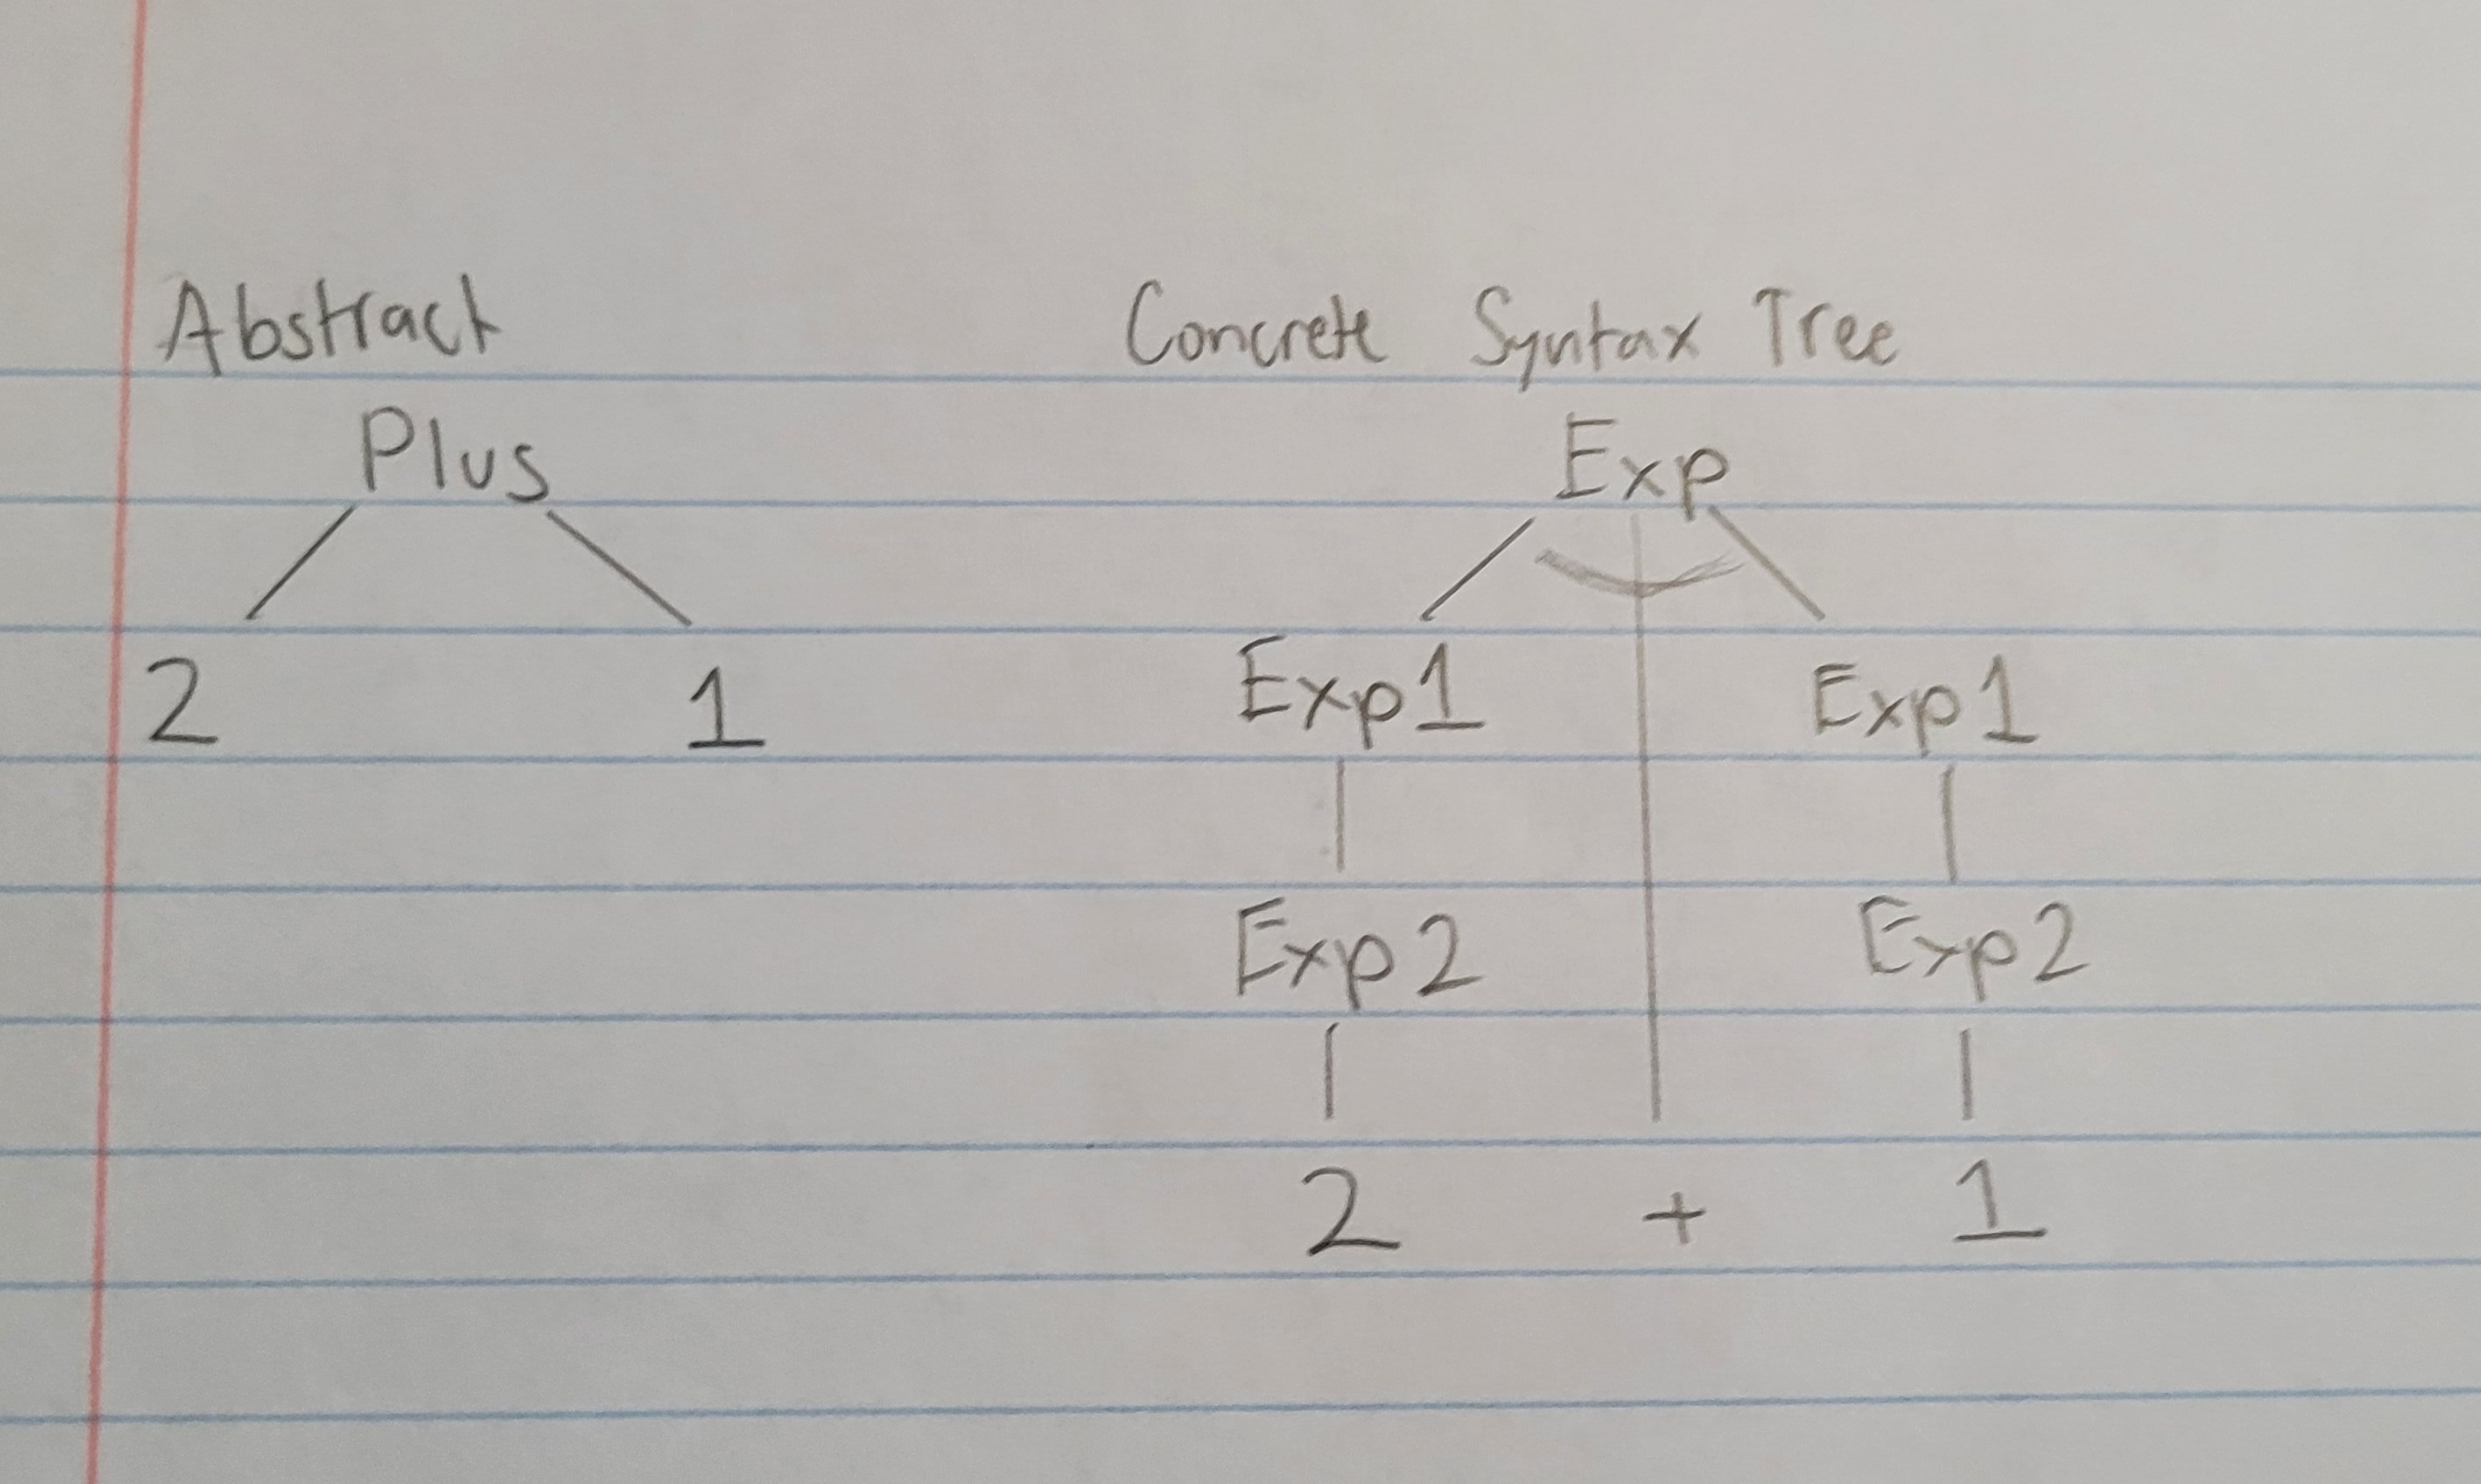
\includegraphics[width=15cm, height=8cm]{Report Images/week4_1.jpg}
\begin{lstlisting}
Plus (Num 2) (Num 1)
\end{lstlisting}


The Abstract Syntax Tree of $1 + 2 * 3$ is:

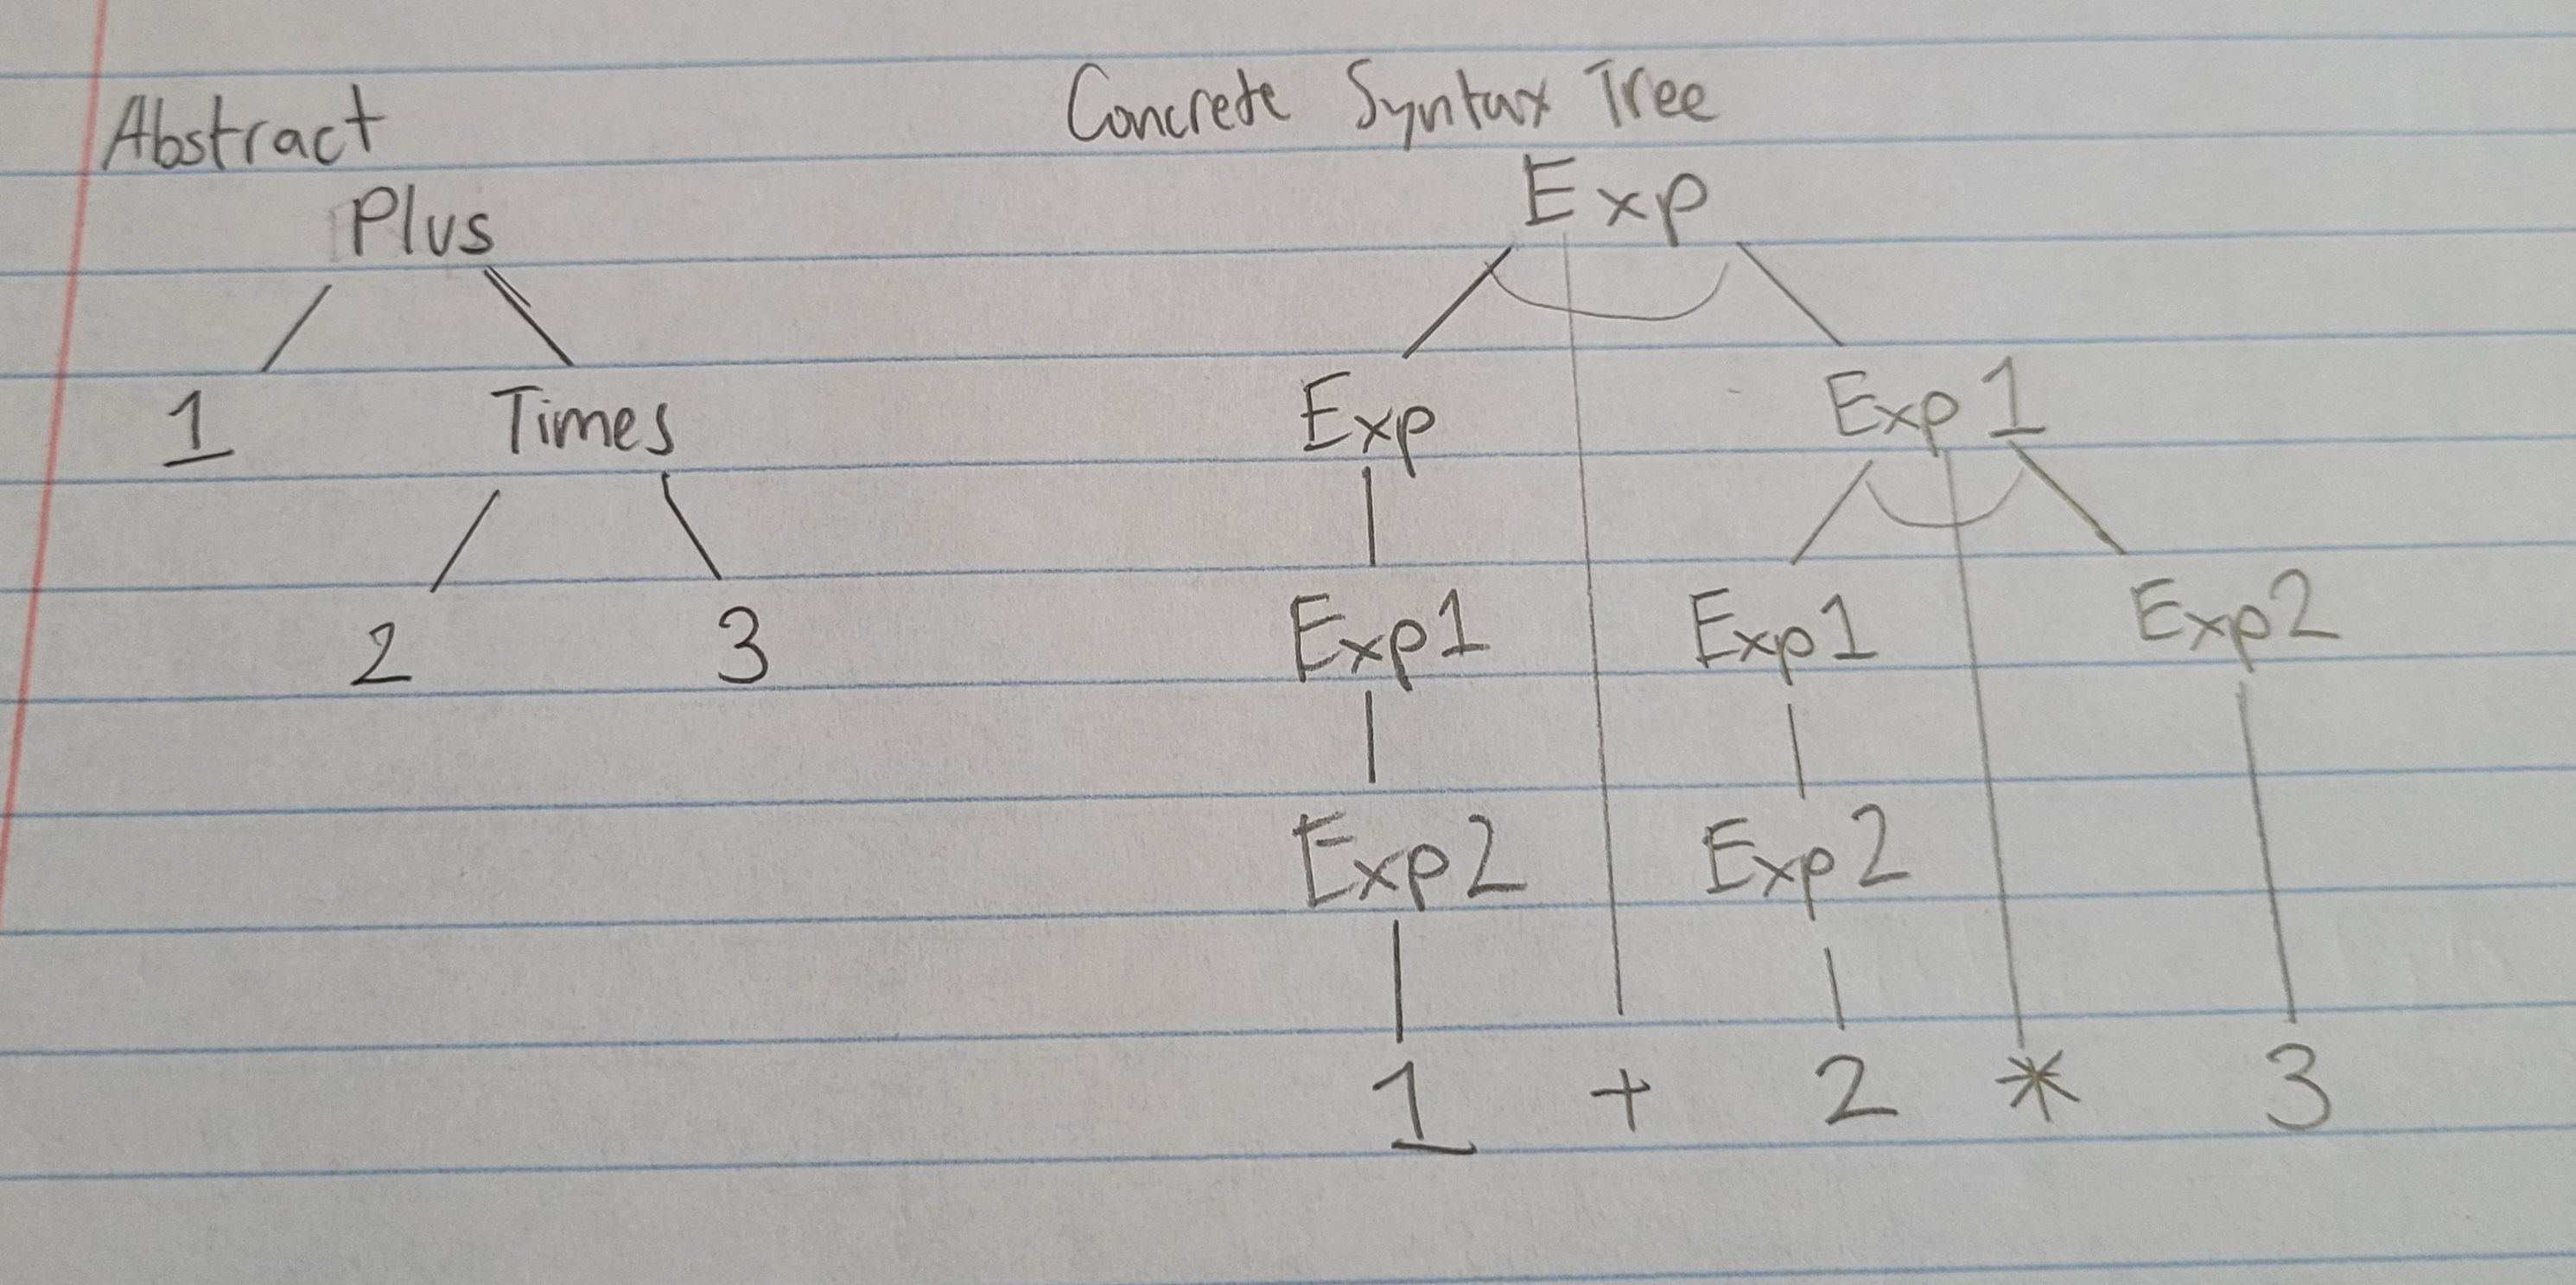
\includegraphics[width=15cm, height=8cm]{Report Images/week4_2.jpg}
\begin{lstlisting}
Plus (Num 1) (Times (Num 2) (Num 3))
\end{lstlisting}

The Abstract Syntax Tree of $1 + (2 * 3)$ is:

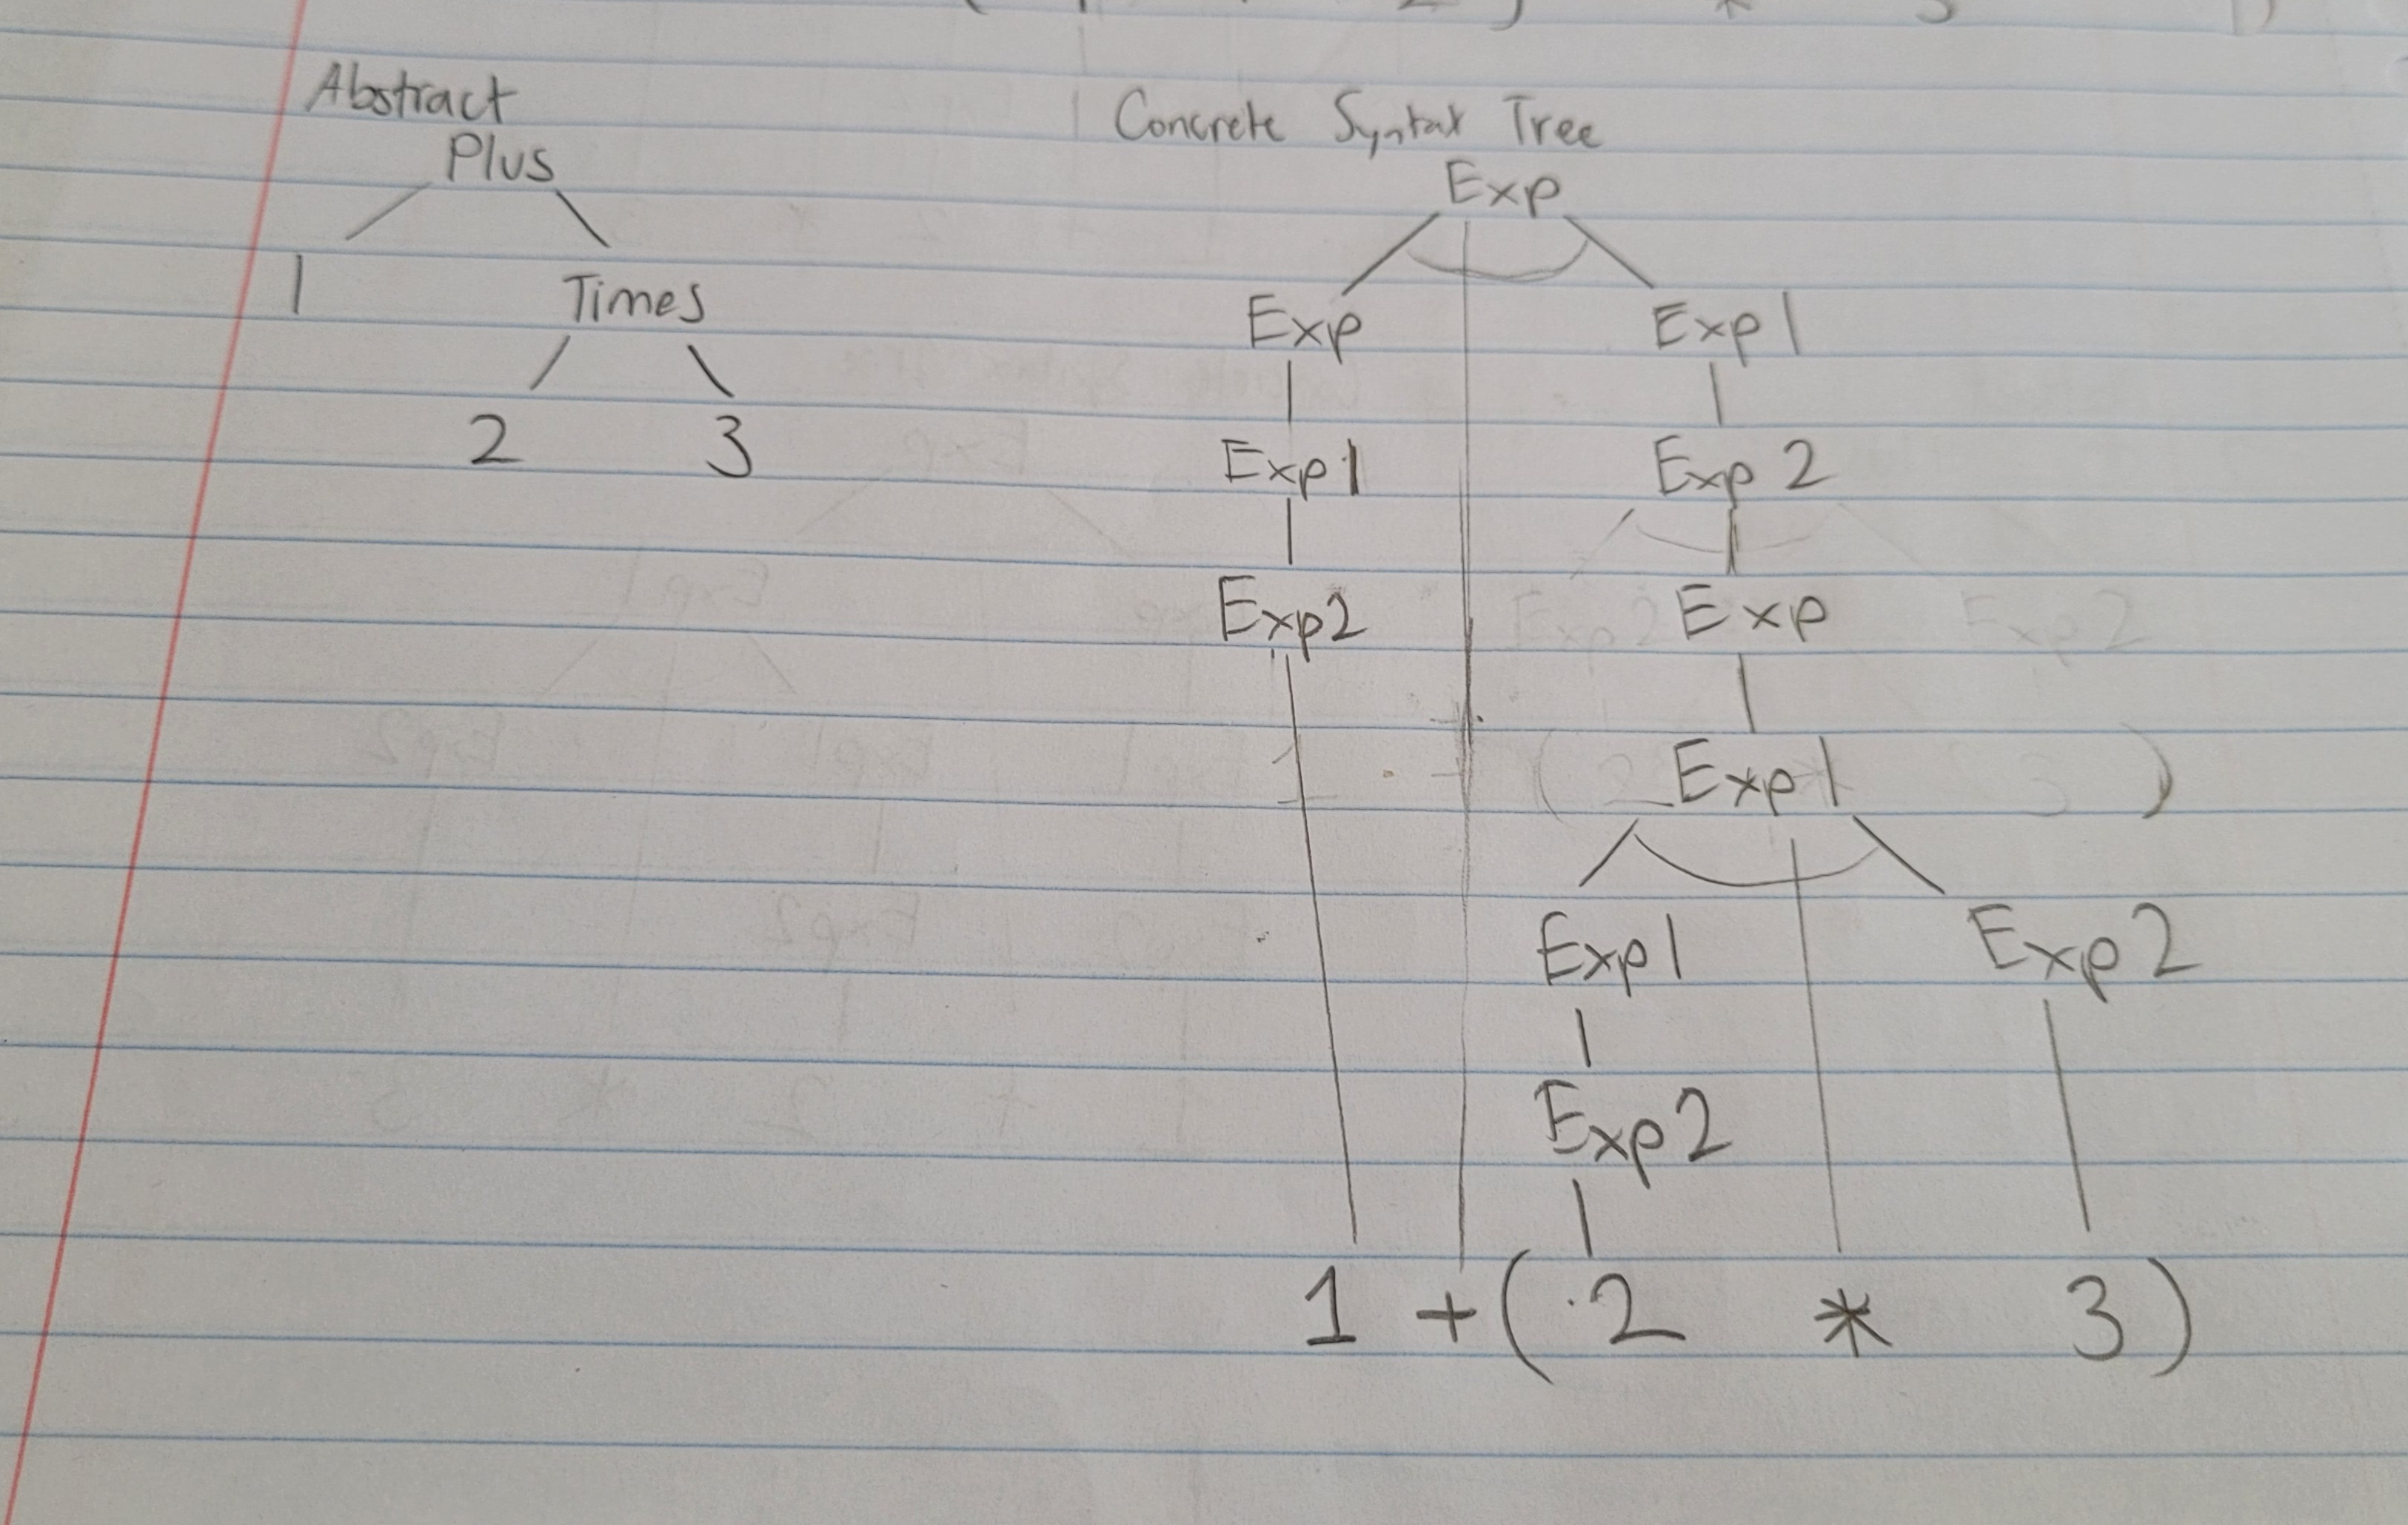
\includegraphics[width=15cm, height=8cm]{Report Images/week4_3.jpg}
\begin{lstlisting}
Plus (Num 1) (Times (Num 2) (Num 3))
\end{lstlisting}

The Abstract Syntax Tree of $(1 + 2) * 3$ is:

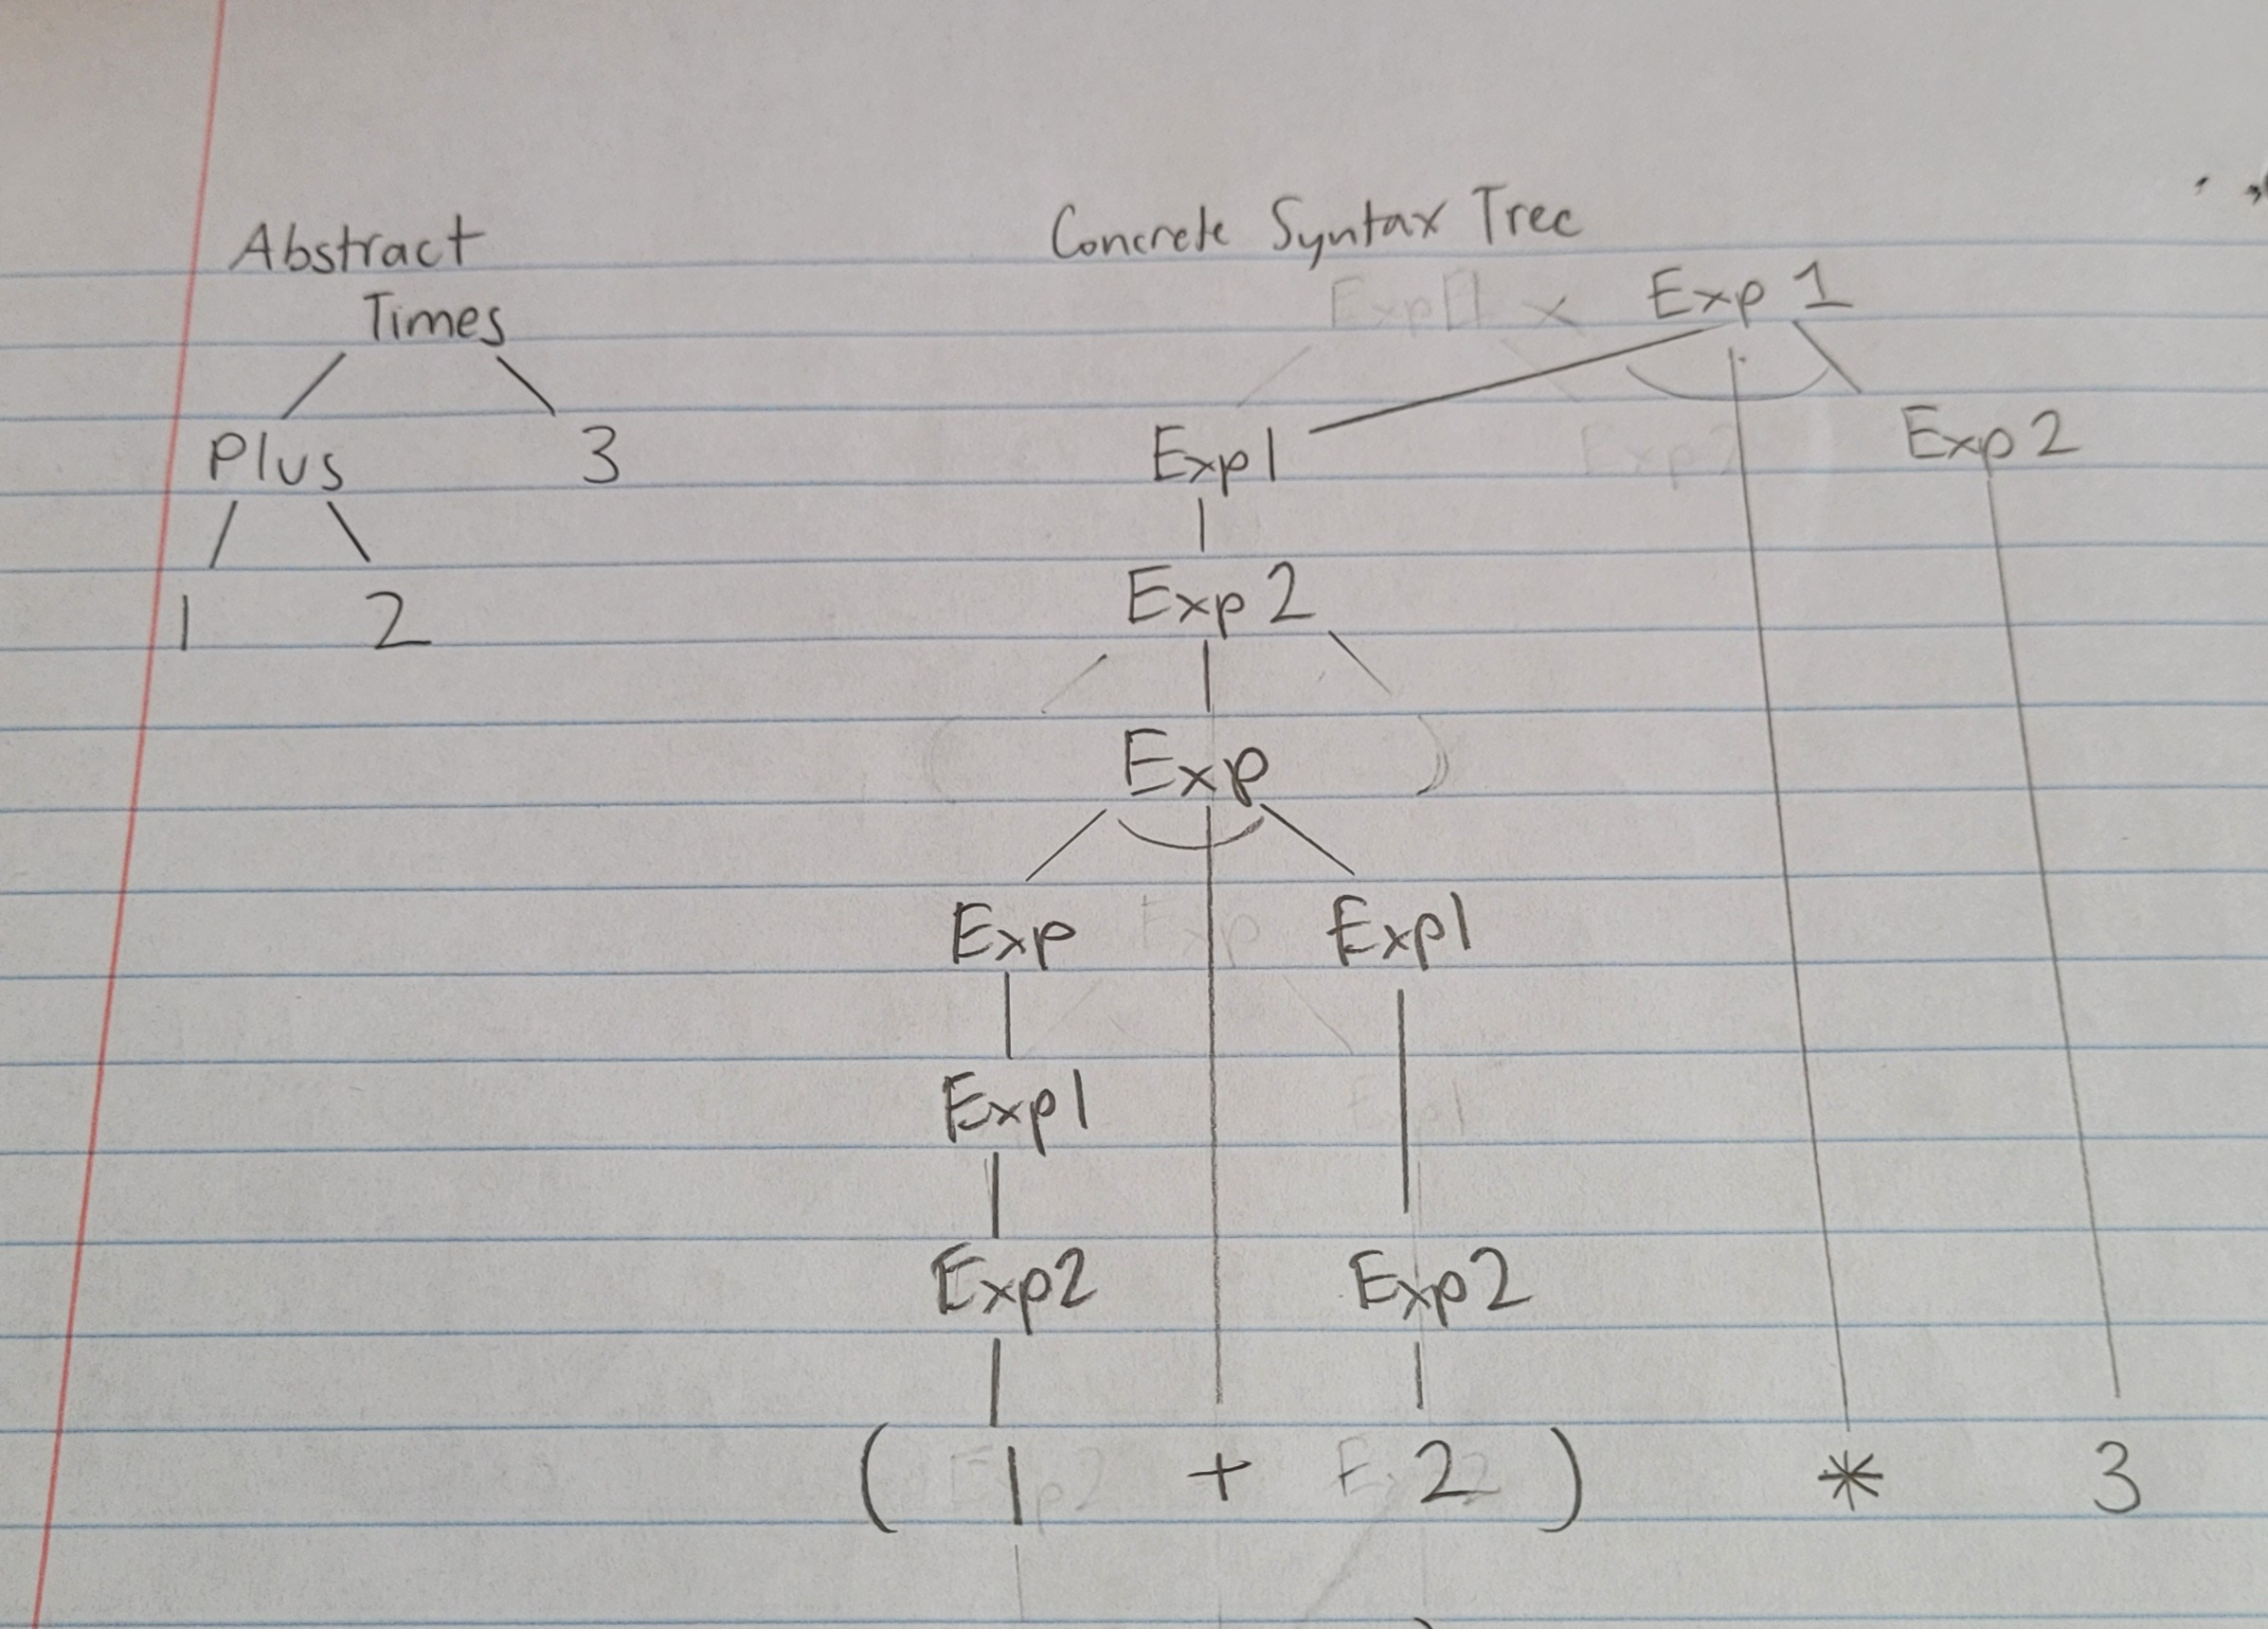
\includegraphics[width=15cm, height=8cm]{Report Images/week4_4.jpg}
\begin{lstlisting}
Times (Plus (Num 1) (Num 2)) (Num 3)
\end{lstlisting}

The Abstract Syntax Tree of $1 + 2 * 3 + 4 * 5 + 6$ is:

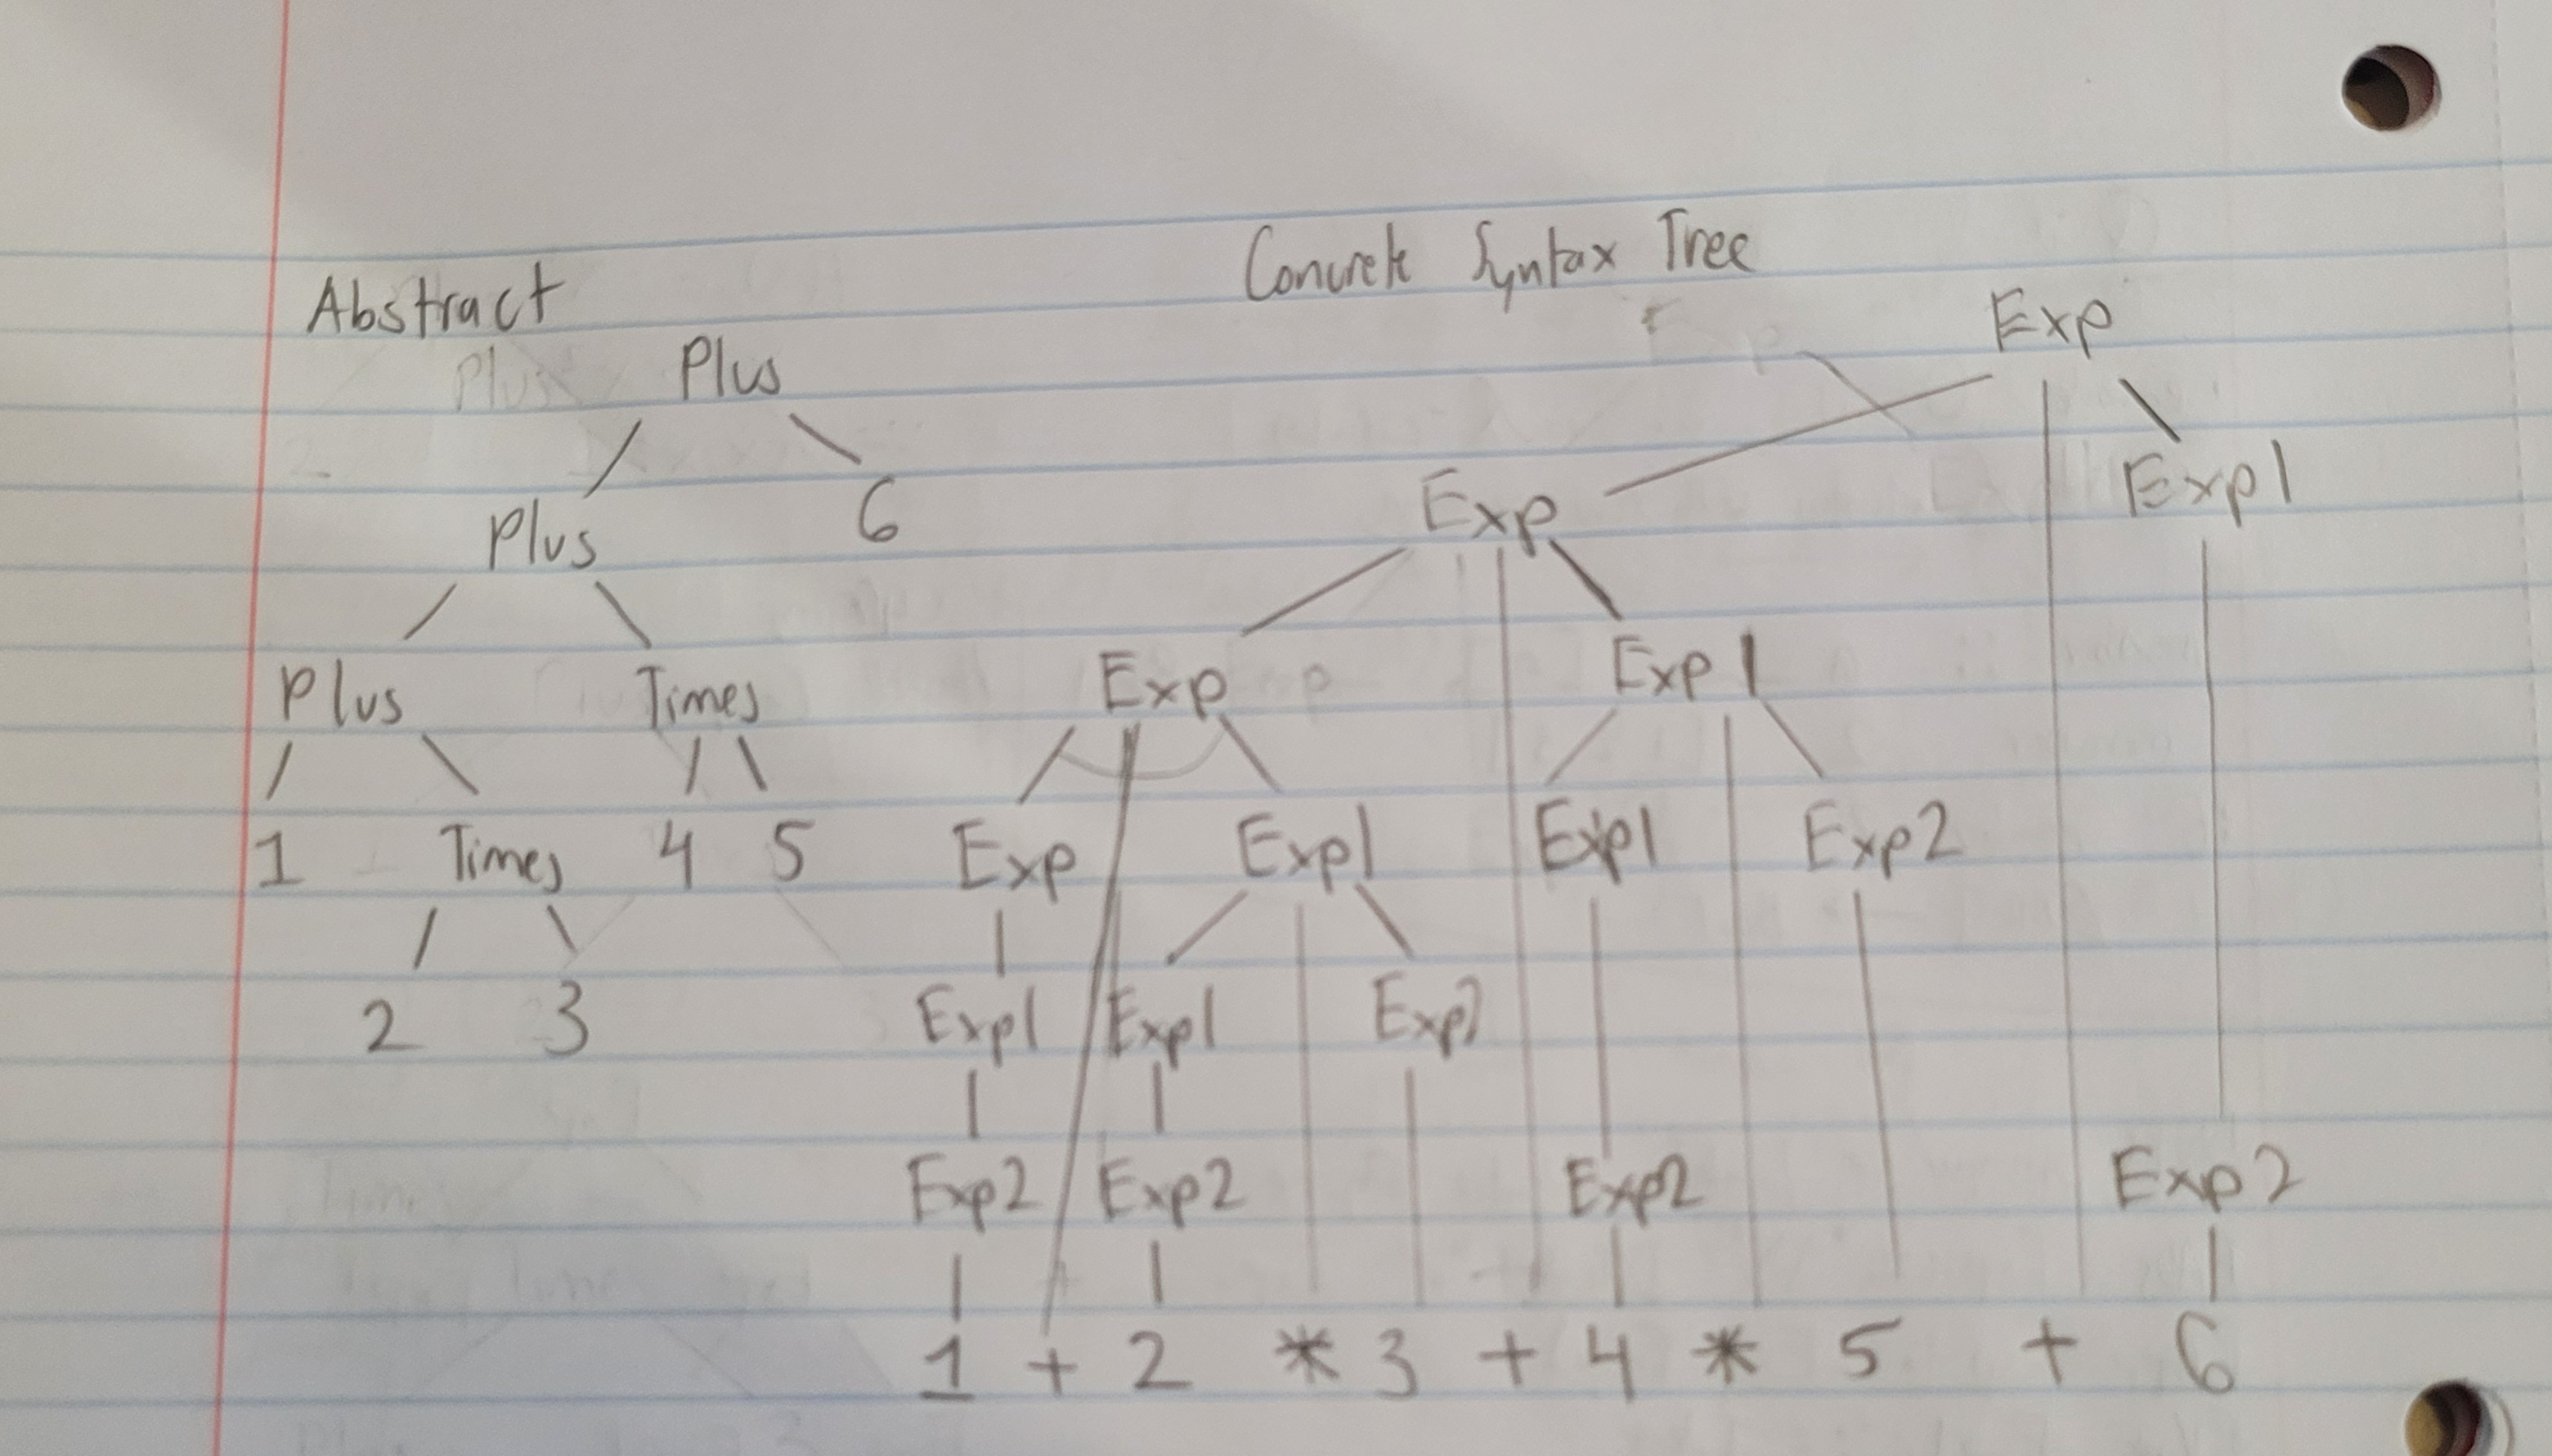
\includegraphics[width=15cm, height=8cm]{Report Images/week4_5.jpg}
\begin{lstlisting}
Plus (Plus (Plus (Num 1) (Times (Num 2) (Num 3))) (Times (Num 4) (Num 5))) (Num 6)
\end{lstlisting}


The abstract syntax tree of $1+2+3$ would be identical to the one of $(1+2)+3$ as the compiler would calculate from left to right as there are no other higher-order operations aside from addition.

\subsection{Week 5}
\textbf{Part 1:}

The Linearized Tree for $x$ is:
\begin{lstlisting}
x
Prog (EVar (Id "x"))
\end{lstlisting}

Its Abstract Syntax Tree:

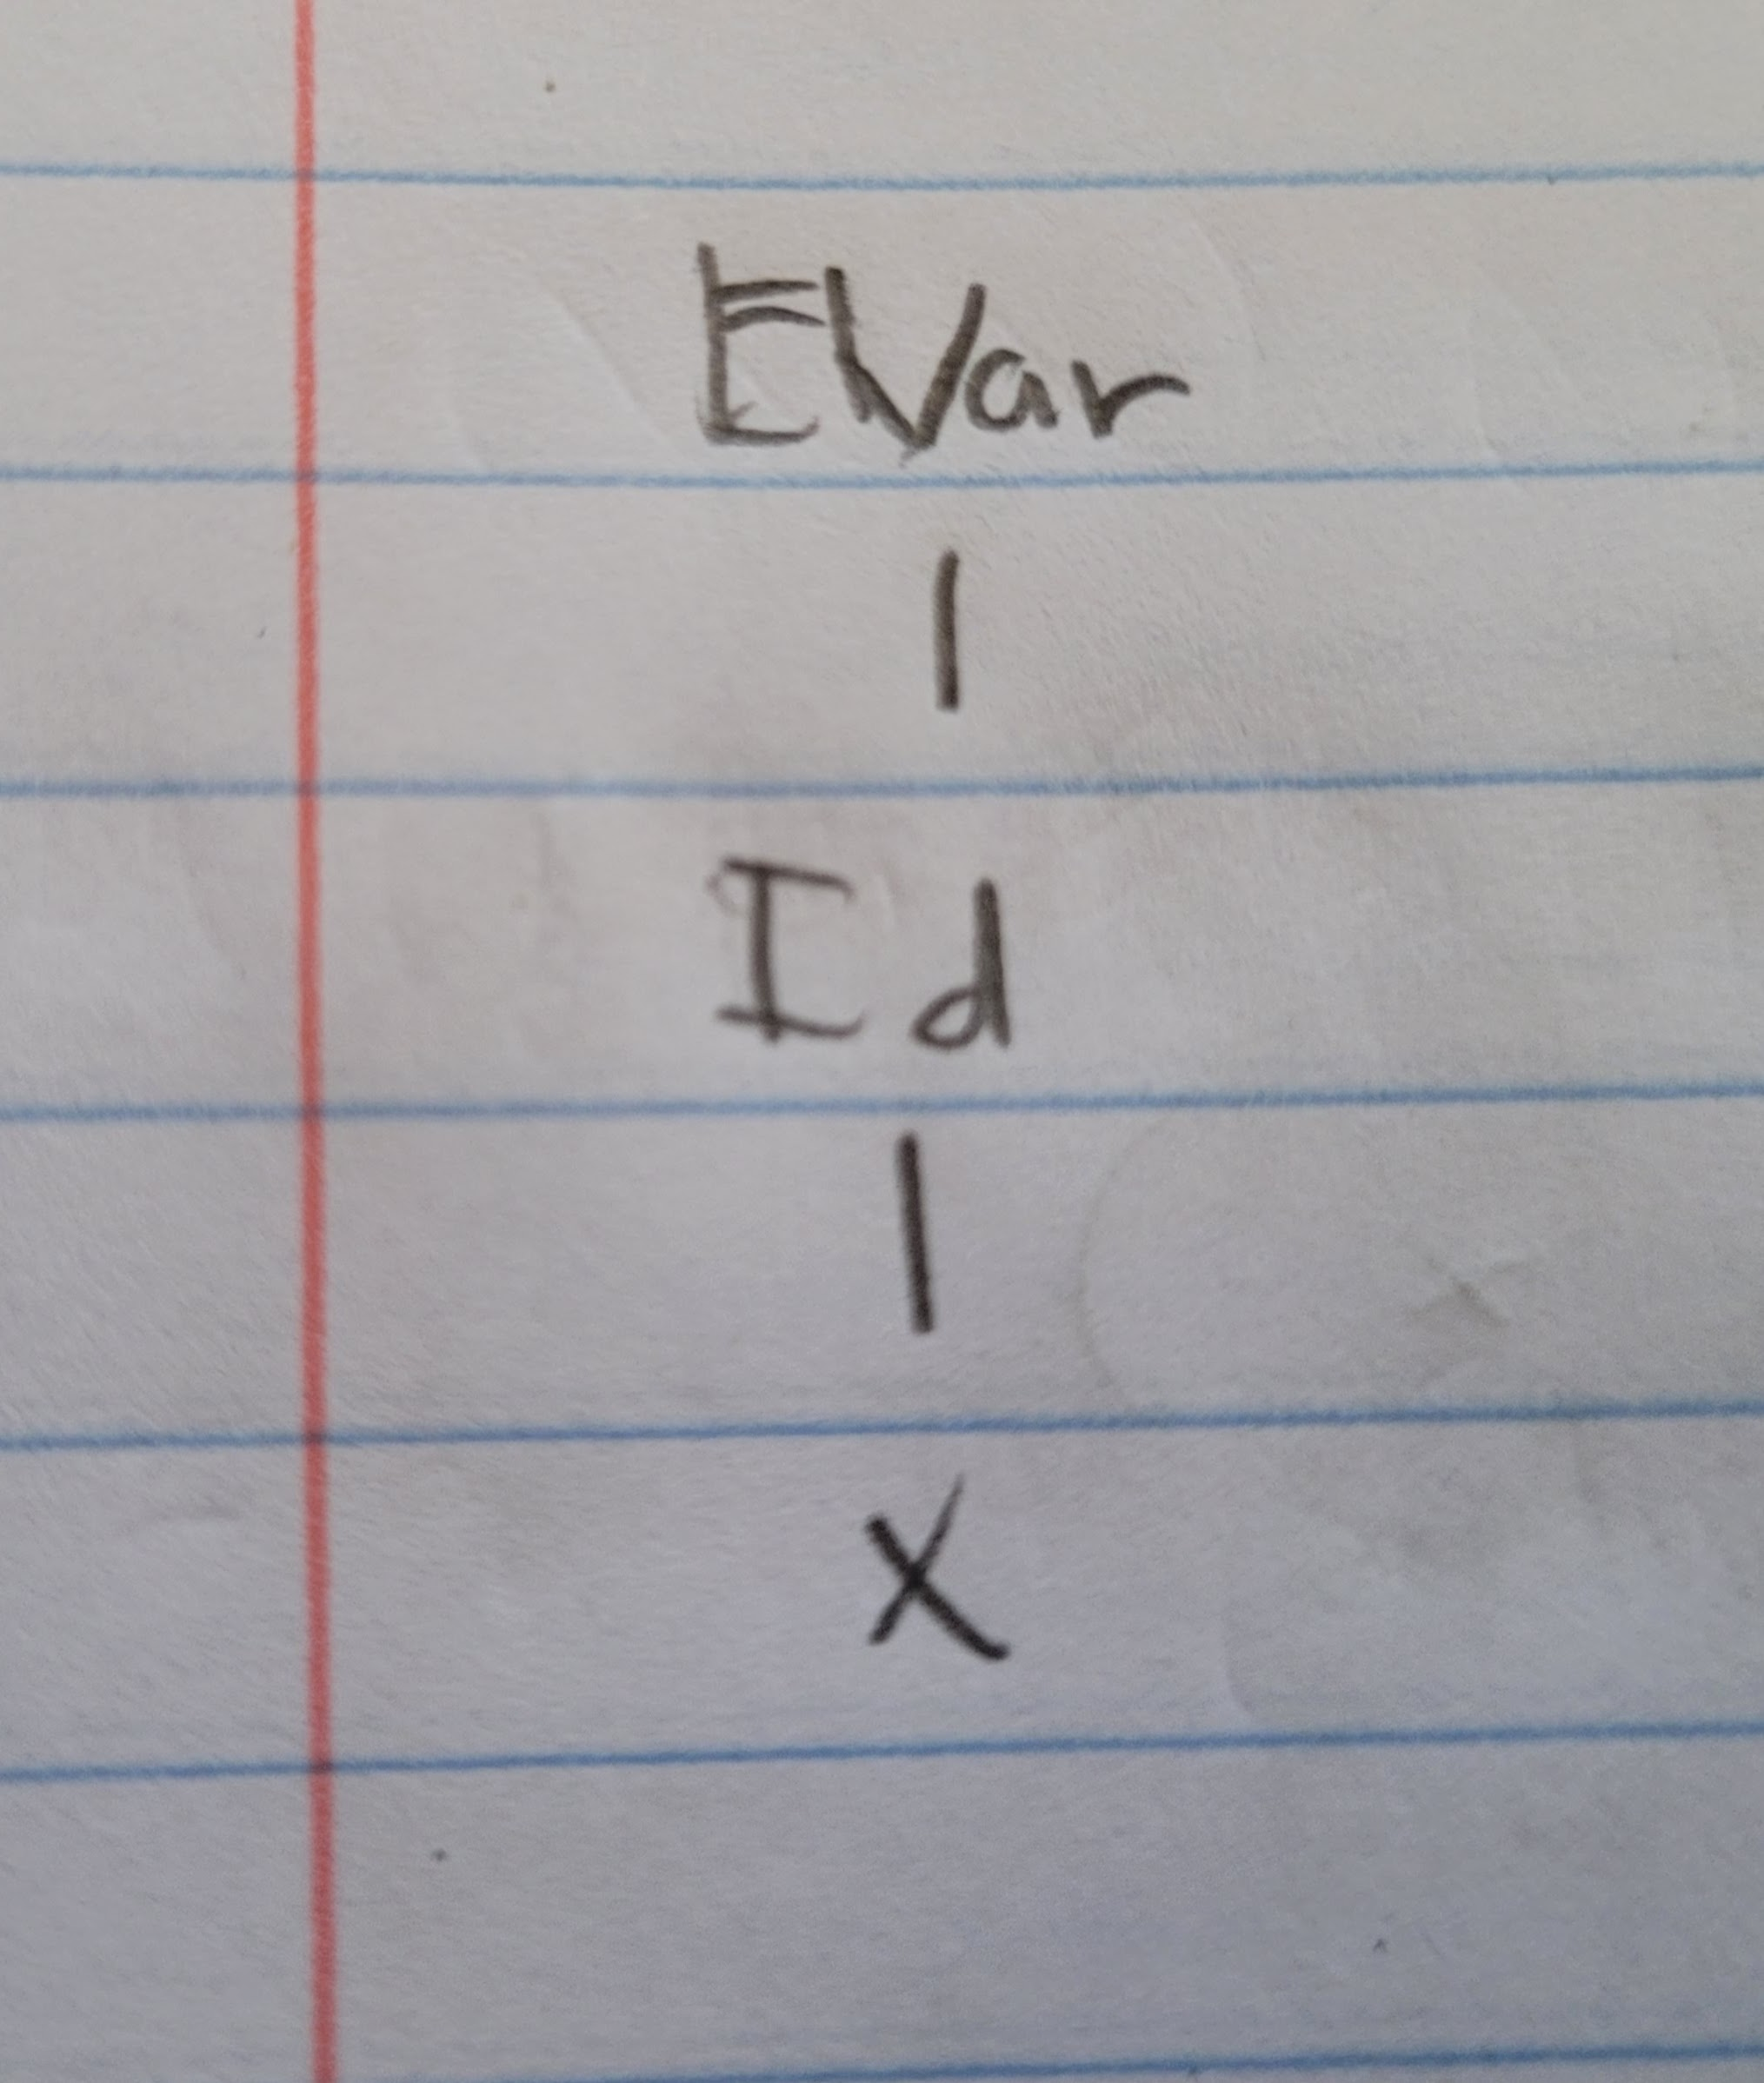
\includegraphics[width=15cm, height=8cm]{Report Images/week5_1.jpg}

The Linearized Tree for x x is:
\begin{lstlisting}
x x
Prog (EApp (EVar (Id "x")) (EVar (Id "x")))
\end{lstlisting}

Its Abstract Syntax Tree:

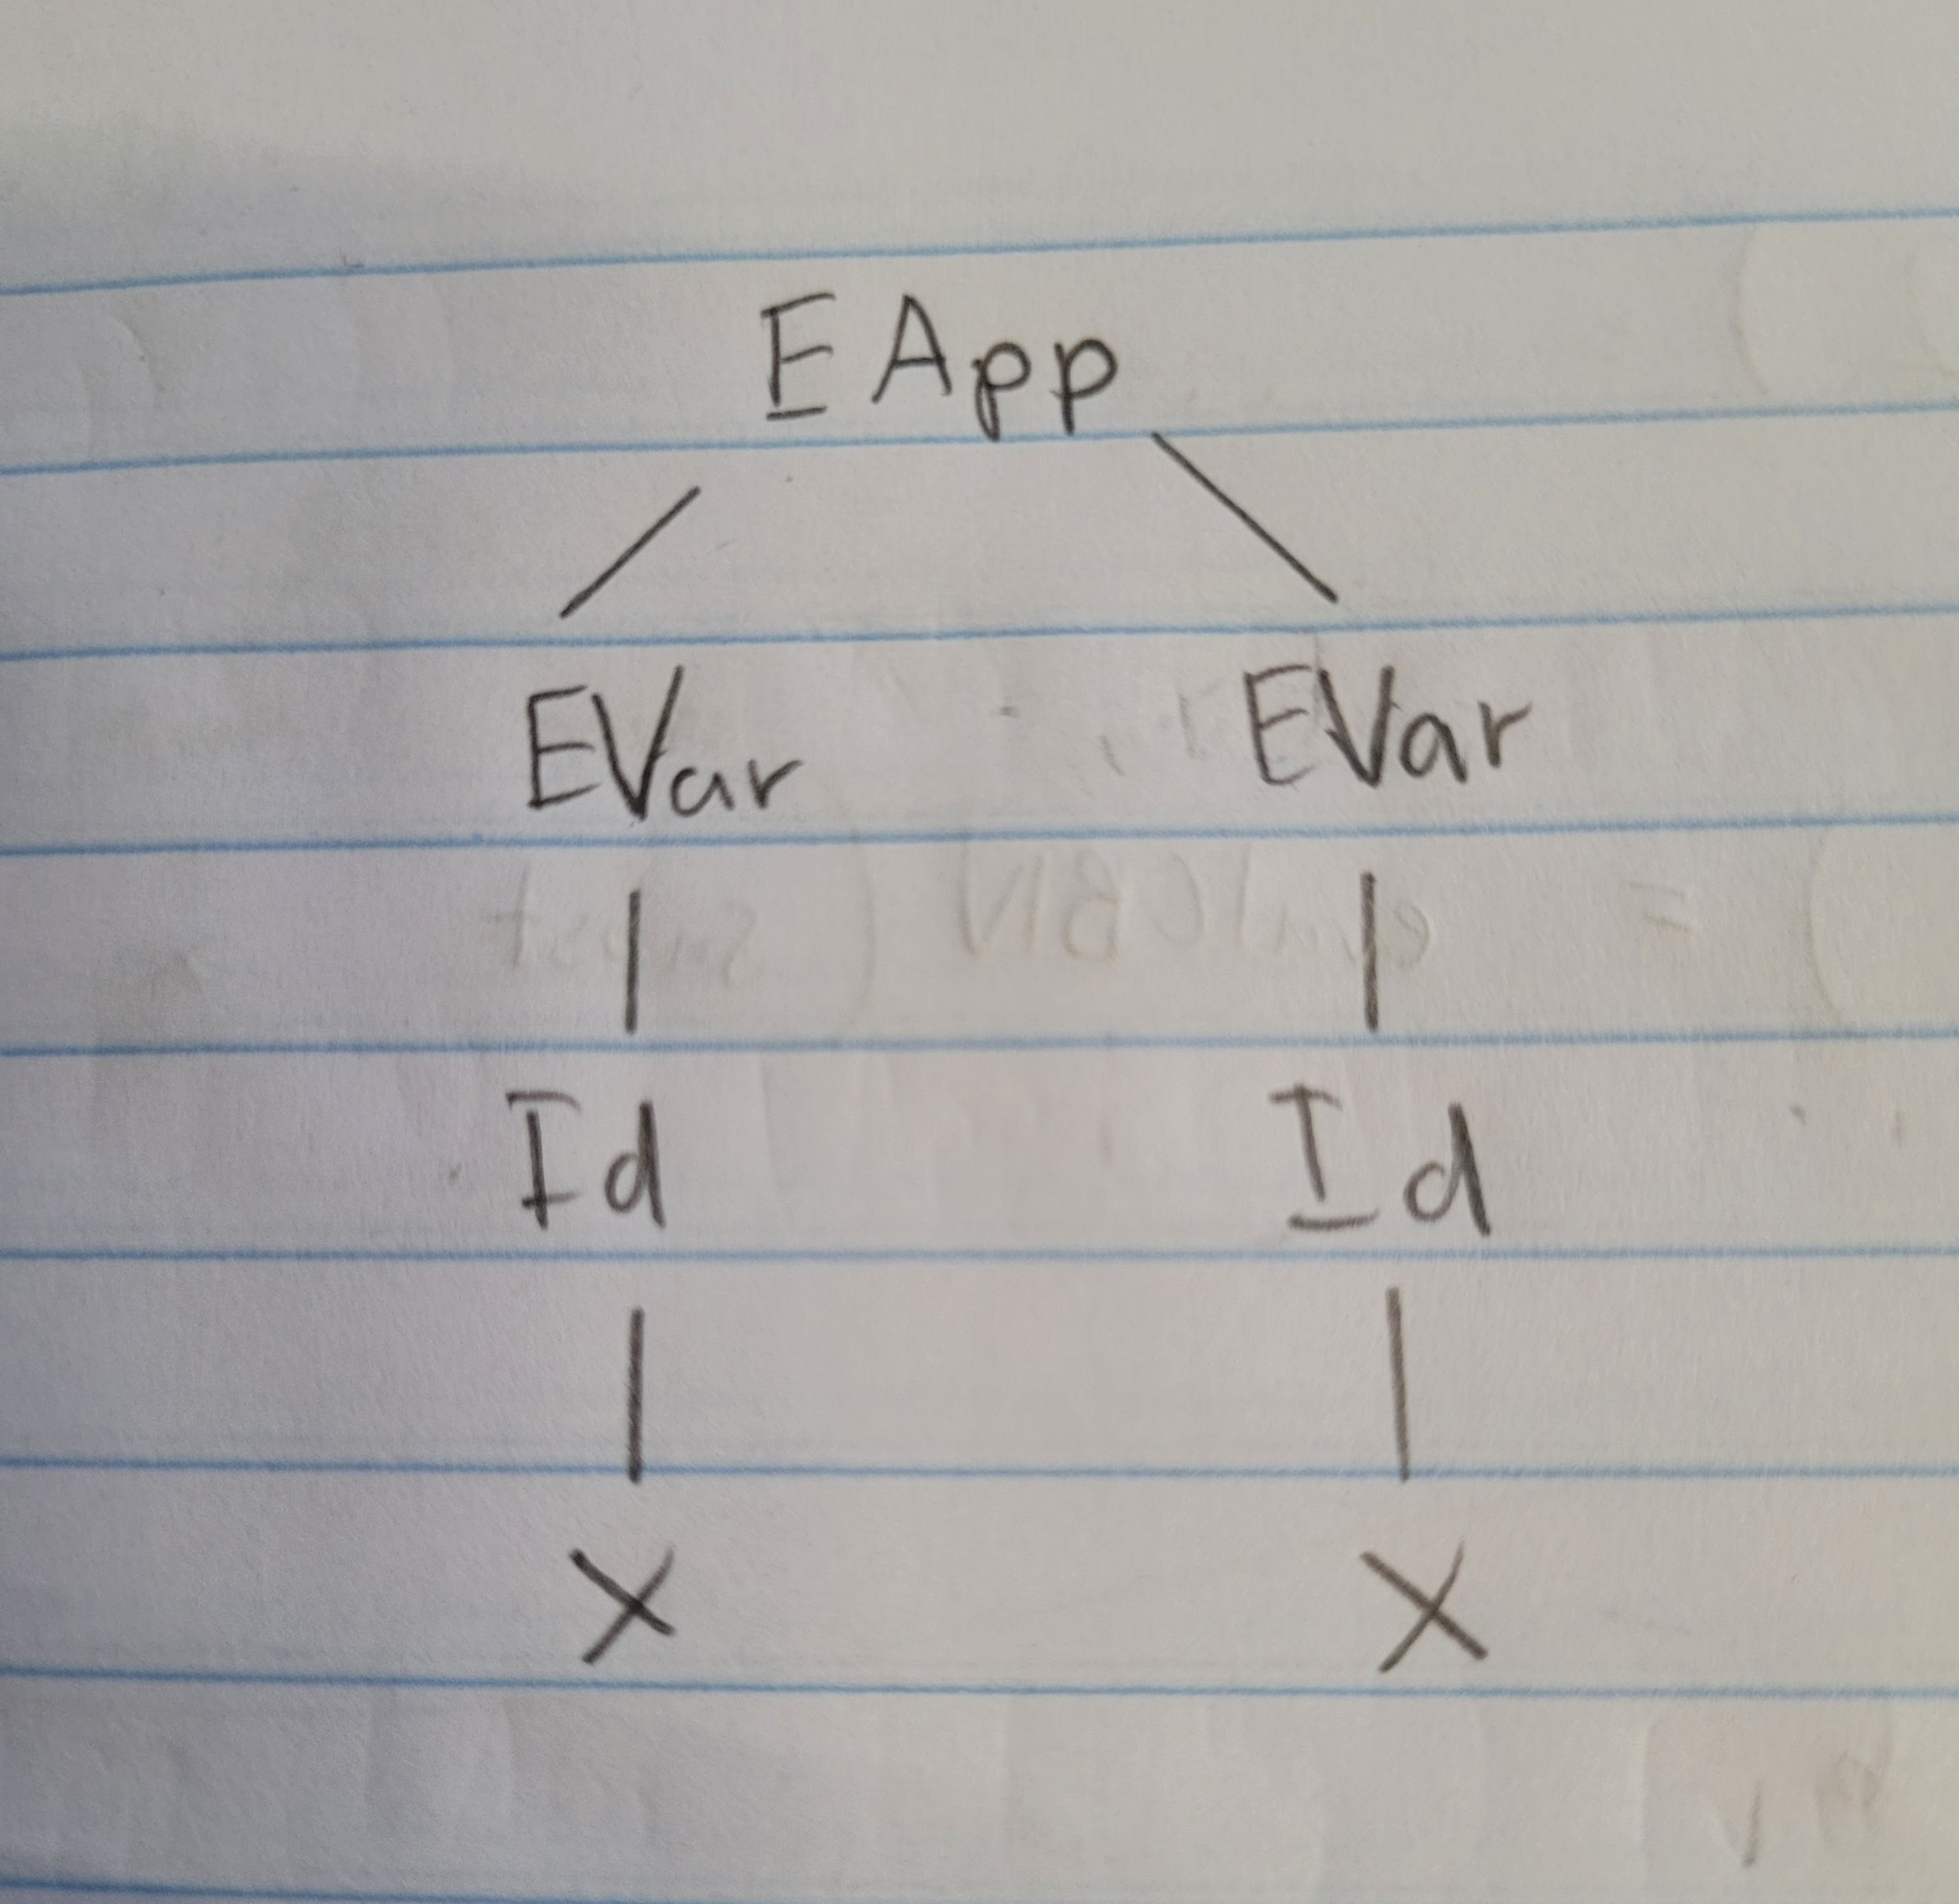
\includegraphics[width=15cm, height=8cm]{Report Images/week5_2.jpg}

The Linearized Tree for x y is:
\begin{lstlisting}
x y
Prog (EApp (EVar (Id "x")) (EVar (Id "y")))
\end{lstlisting}

Its Abstract Syntax Tree:

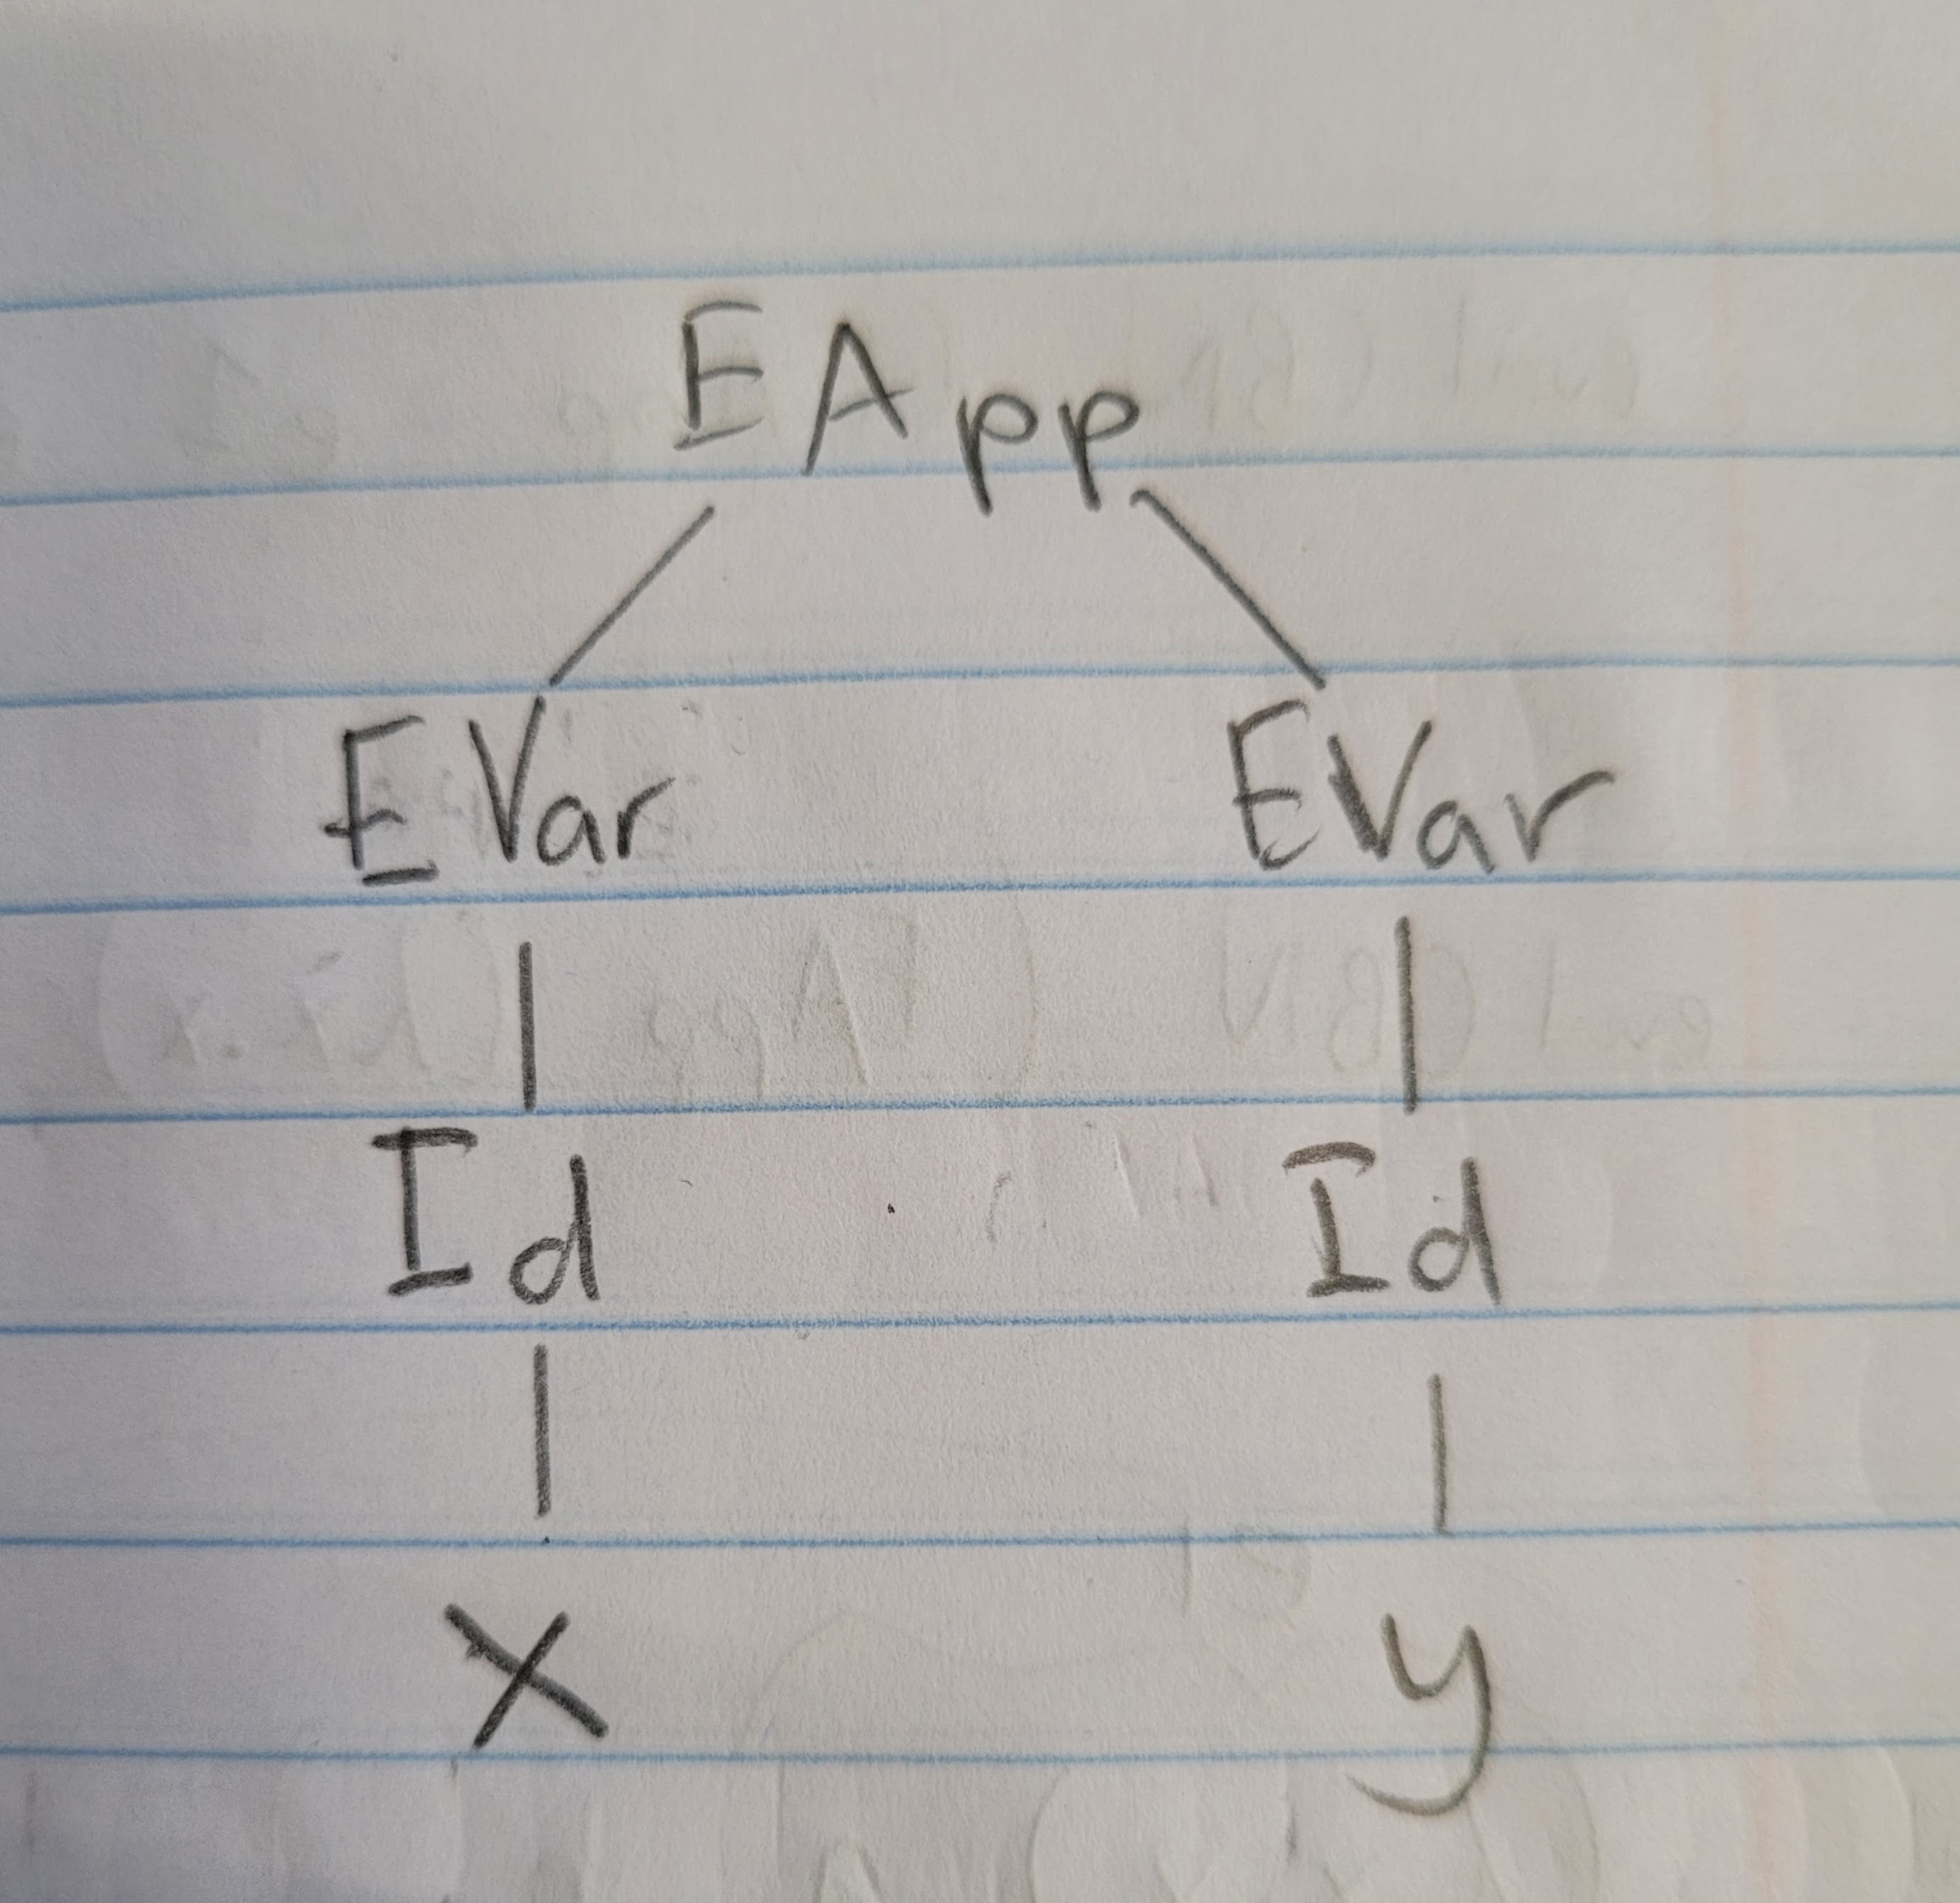
\includegraphics[width=15cm, height=8cm]{Report Images/week5_3.jpg}

The Linearized Tree for x y z is:
\begin{lstlisting}
x y z
Prog (EApp (EApp (EVar (Id "x")) (EVar (Id "y"))) (EVar (Id "z")))
\end{lstlisting}

Its Abstract Syntax Tree:

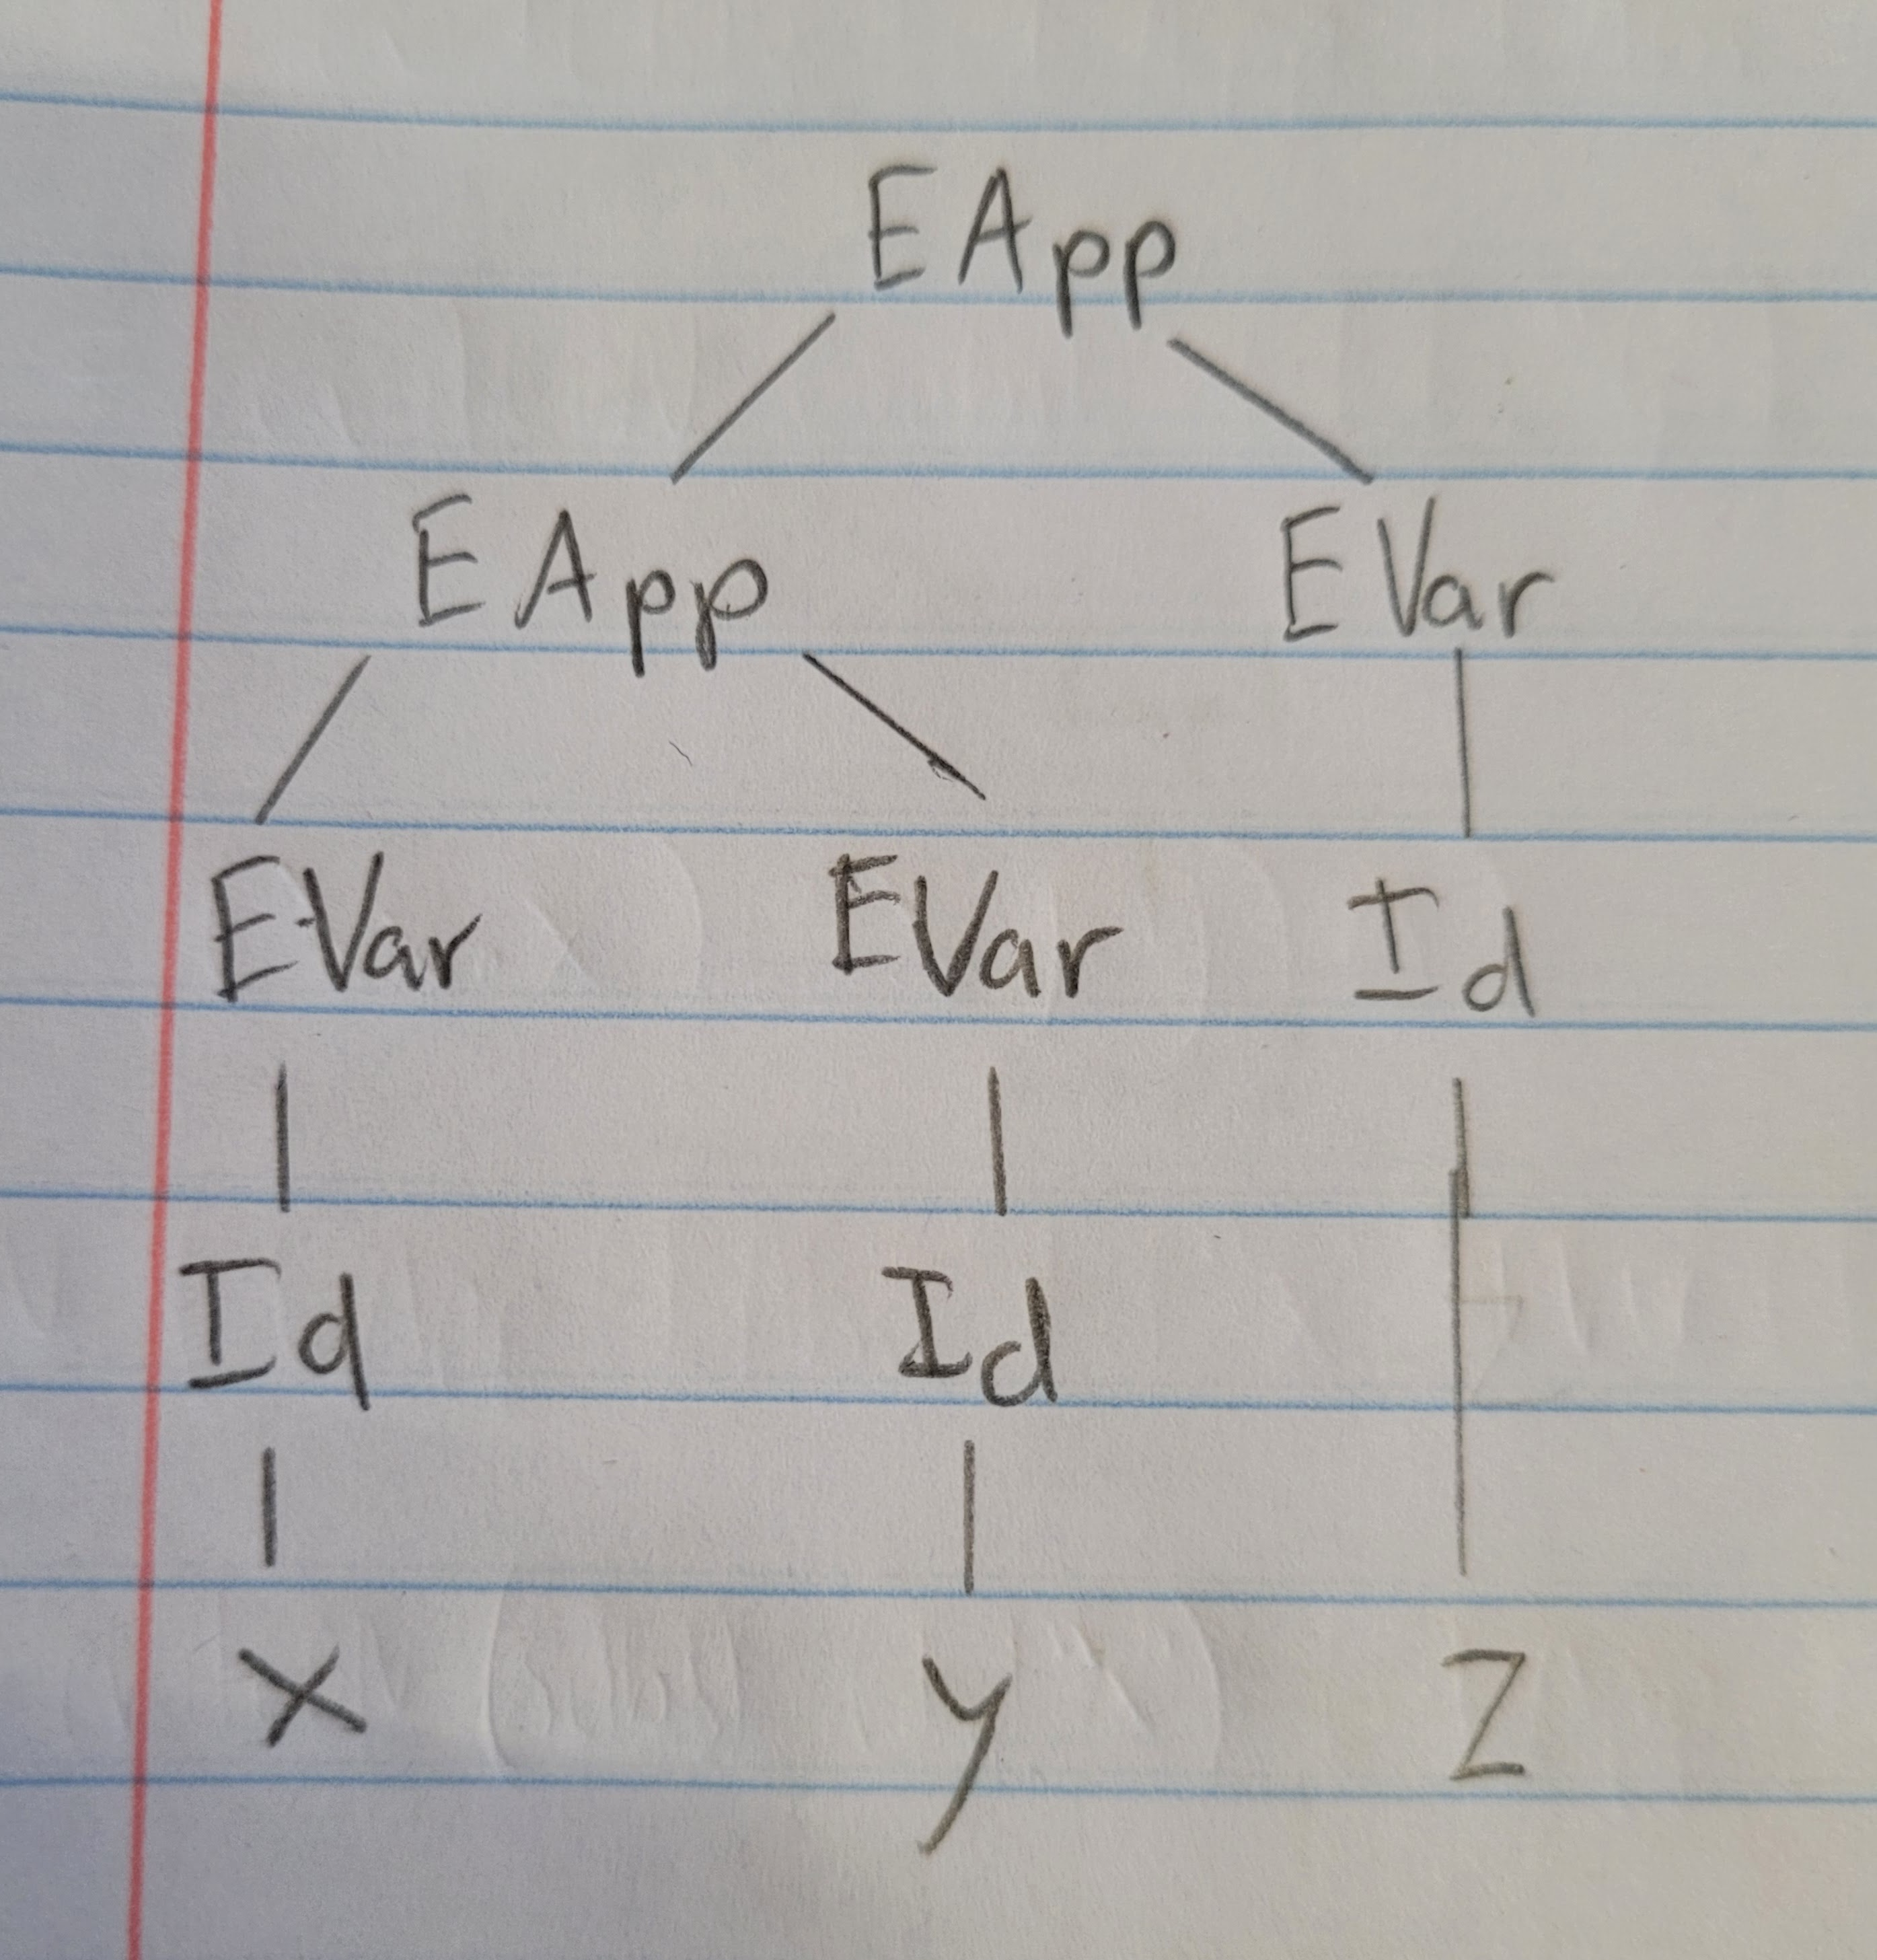
\includegraphics[width=15cm, height=8cm]{Report Images/week5_4.jpg}

The Linearized Tree for \textbackslash  x.x is:
\begin{lstlisting}
\ x . x
Prog (EAbs (Id "x") (EVar (Id "x")))
\end{lstlisting}

Its Abstract Syntax Tree:

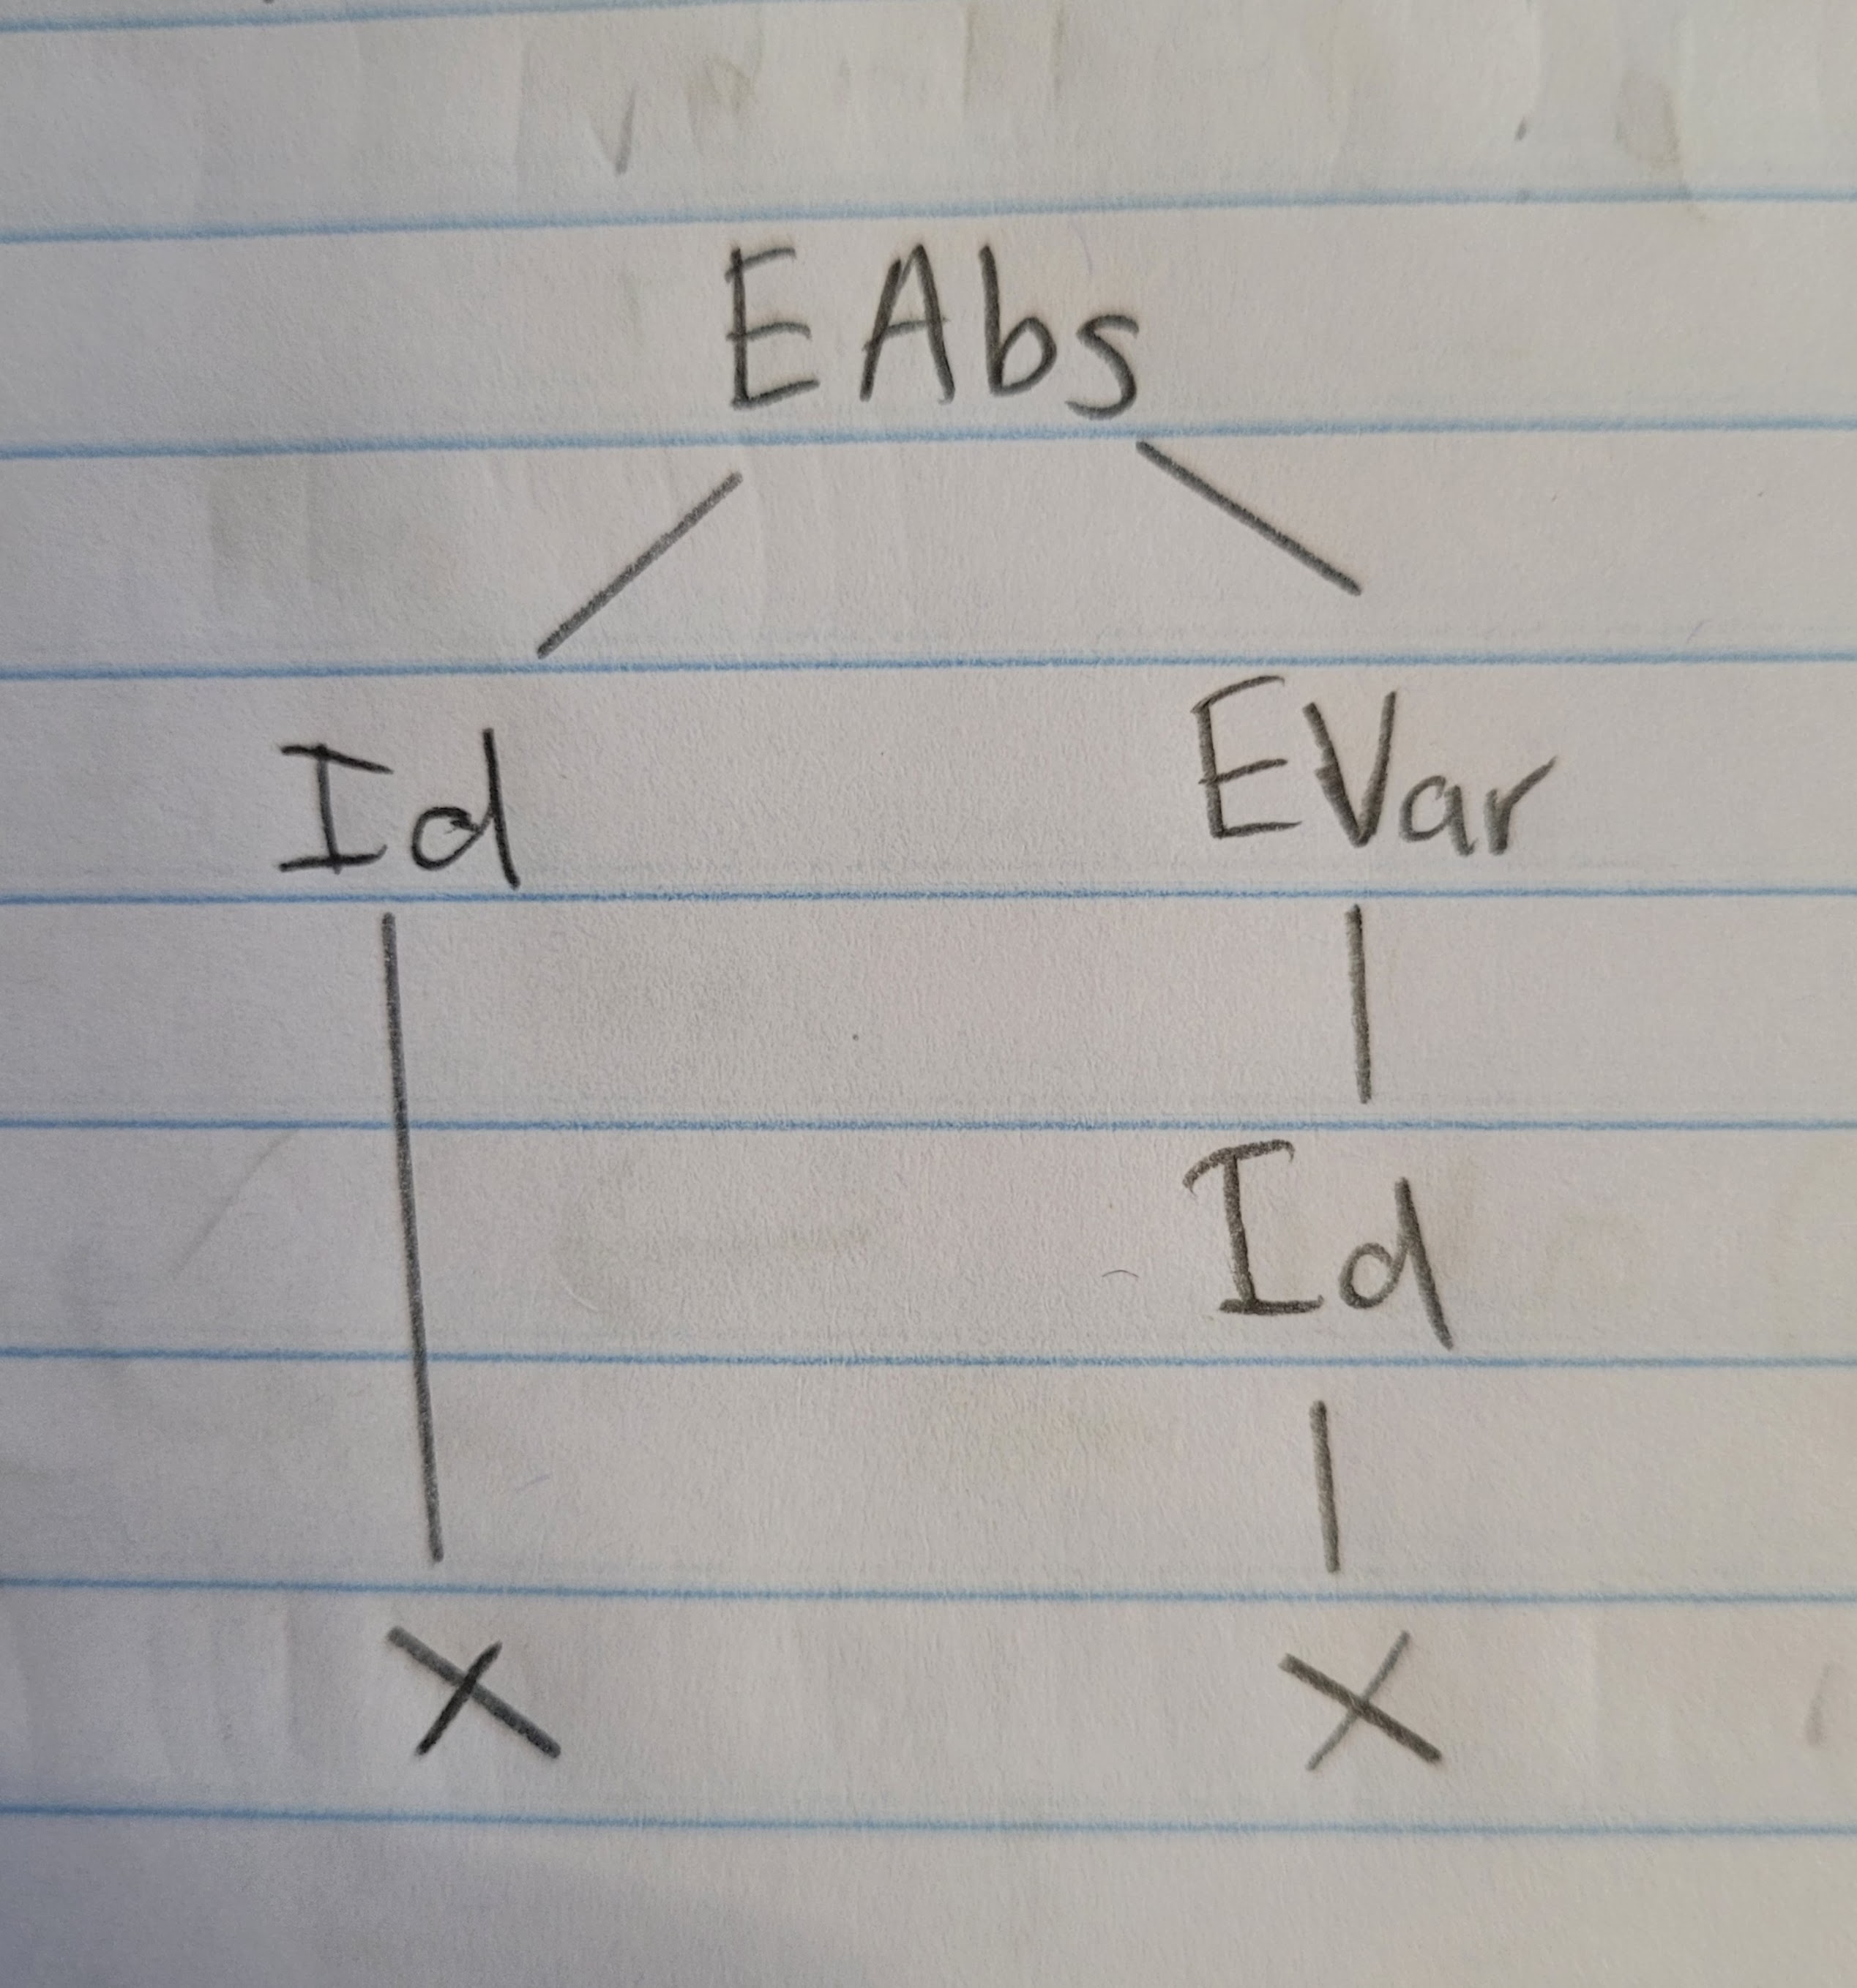
\includegraphics[width=15cm, height=8cm]{Report Images/week5_5.jpg}

The Linearized Tree for \textbackslash x.x x is:
\begin{lstlisting}
\ x . x x
Prog (EAbs (Id "x") (EApp (EVar (Id "x")) (EVar (Id "x"))))
\end{lstlisting}

Its Abstract Syntax Tree:

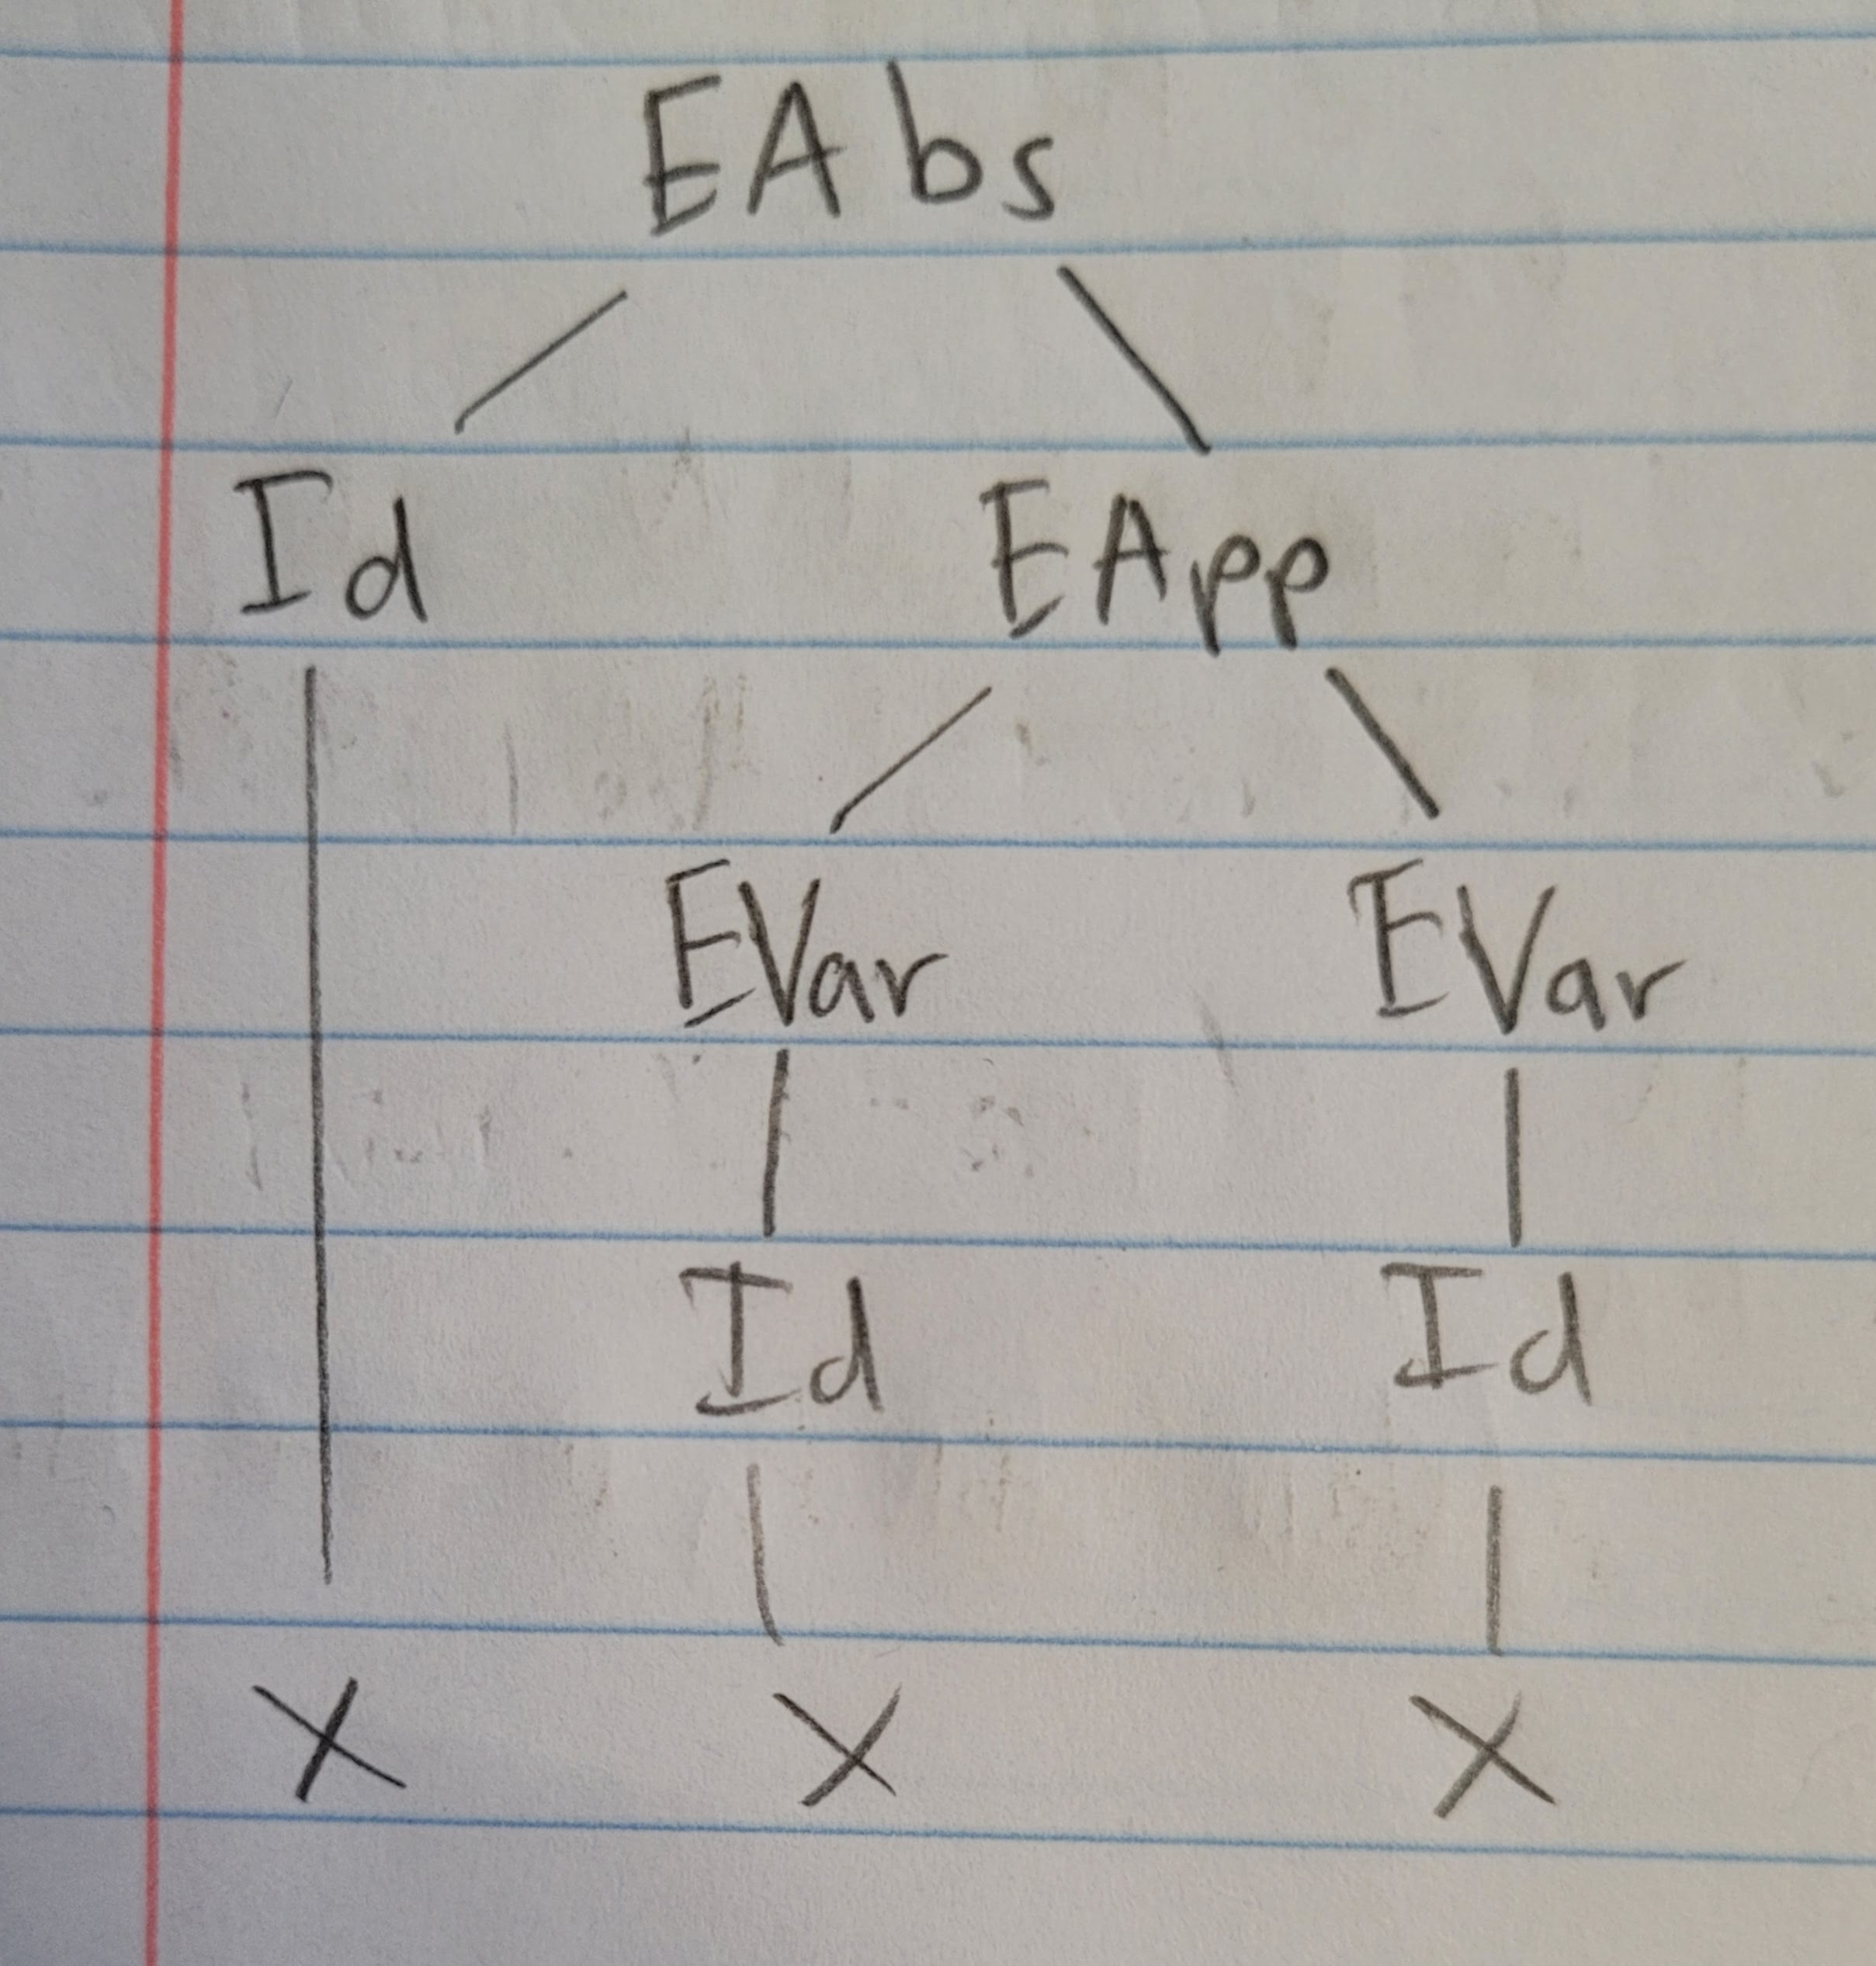
\includegraphics[width=15cm, height=8cm]{Report Images/week5_6.jpg}

The Linearized Tree for (\textbackslash x . (\textbackslash y . x y)) (\textbackslash x.x) z is:
\begin{lstlisting}
\ x . \ y . x y (\ x . x)z
Prog (EApp (EApp (EAbs (Id "x") (EAbs (Id "y") (EApp (EVar (Id "x")) (EVar (Id "y"))))) (EAbs (Id "x") (EVar (Id "x")))) (EVar (Id "z")))
\end{lstlisting}

Its Abstract Syntax Tree:

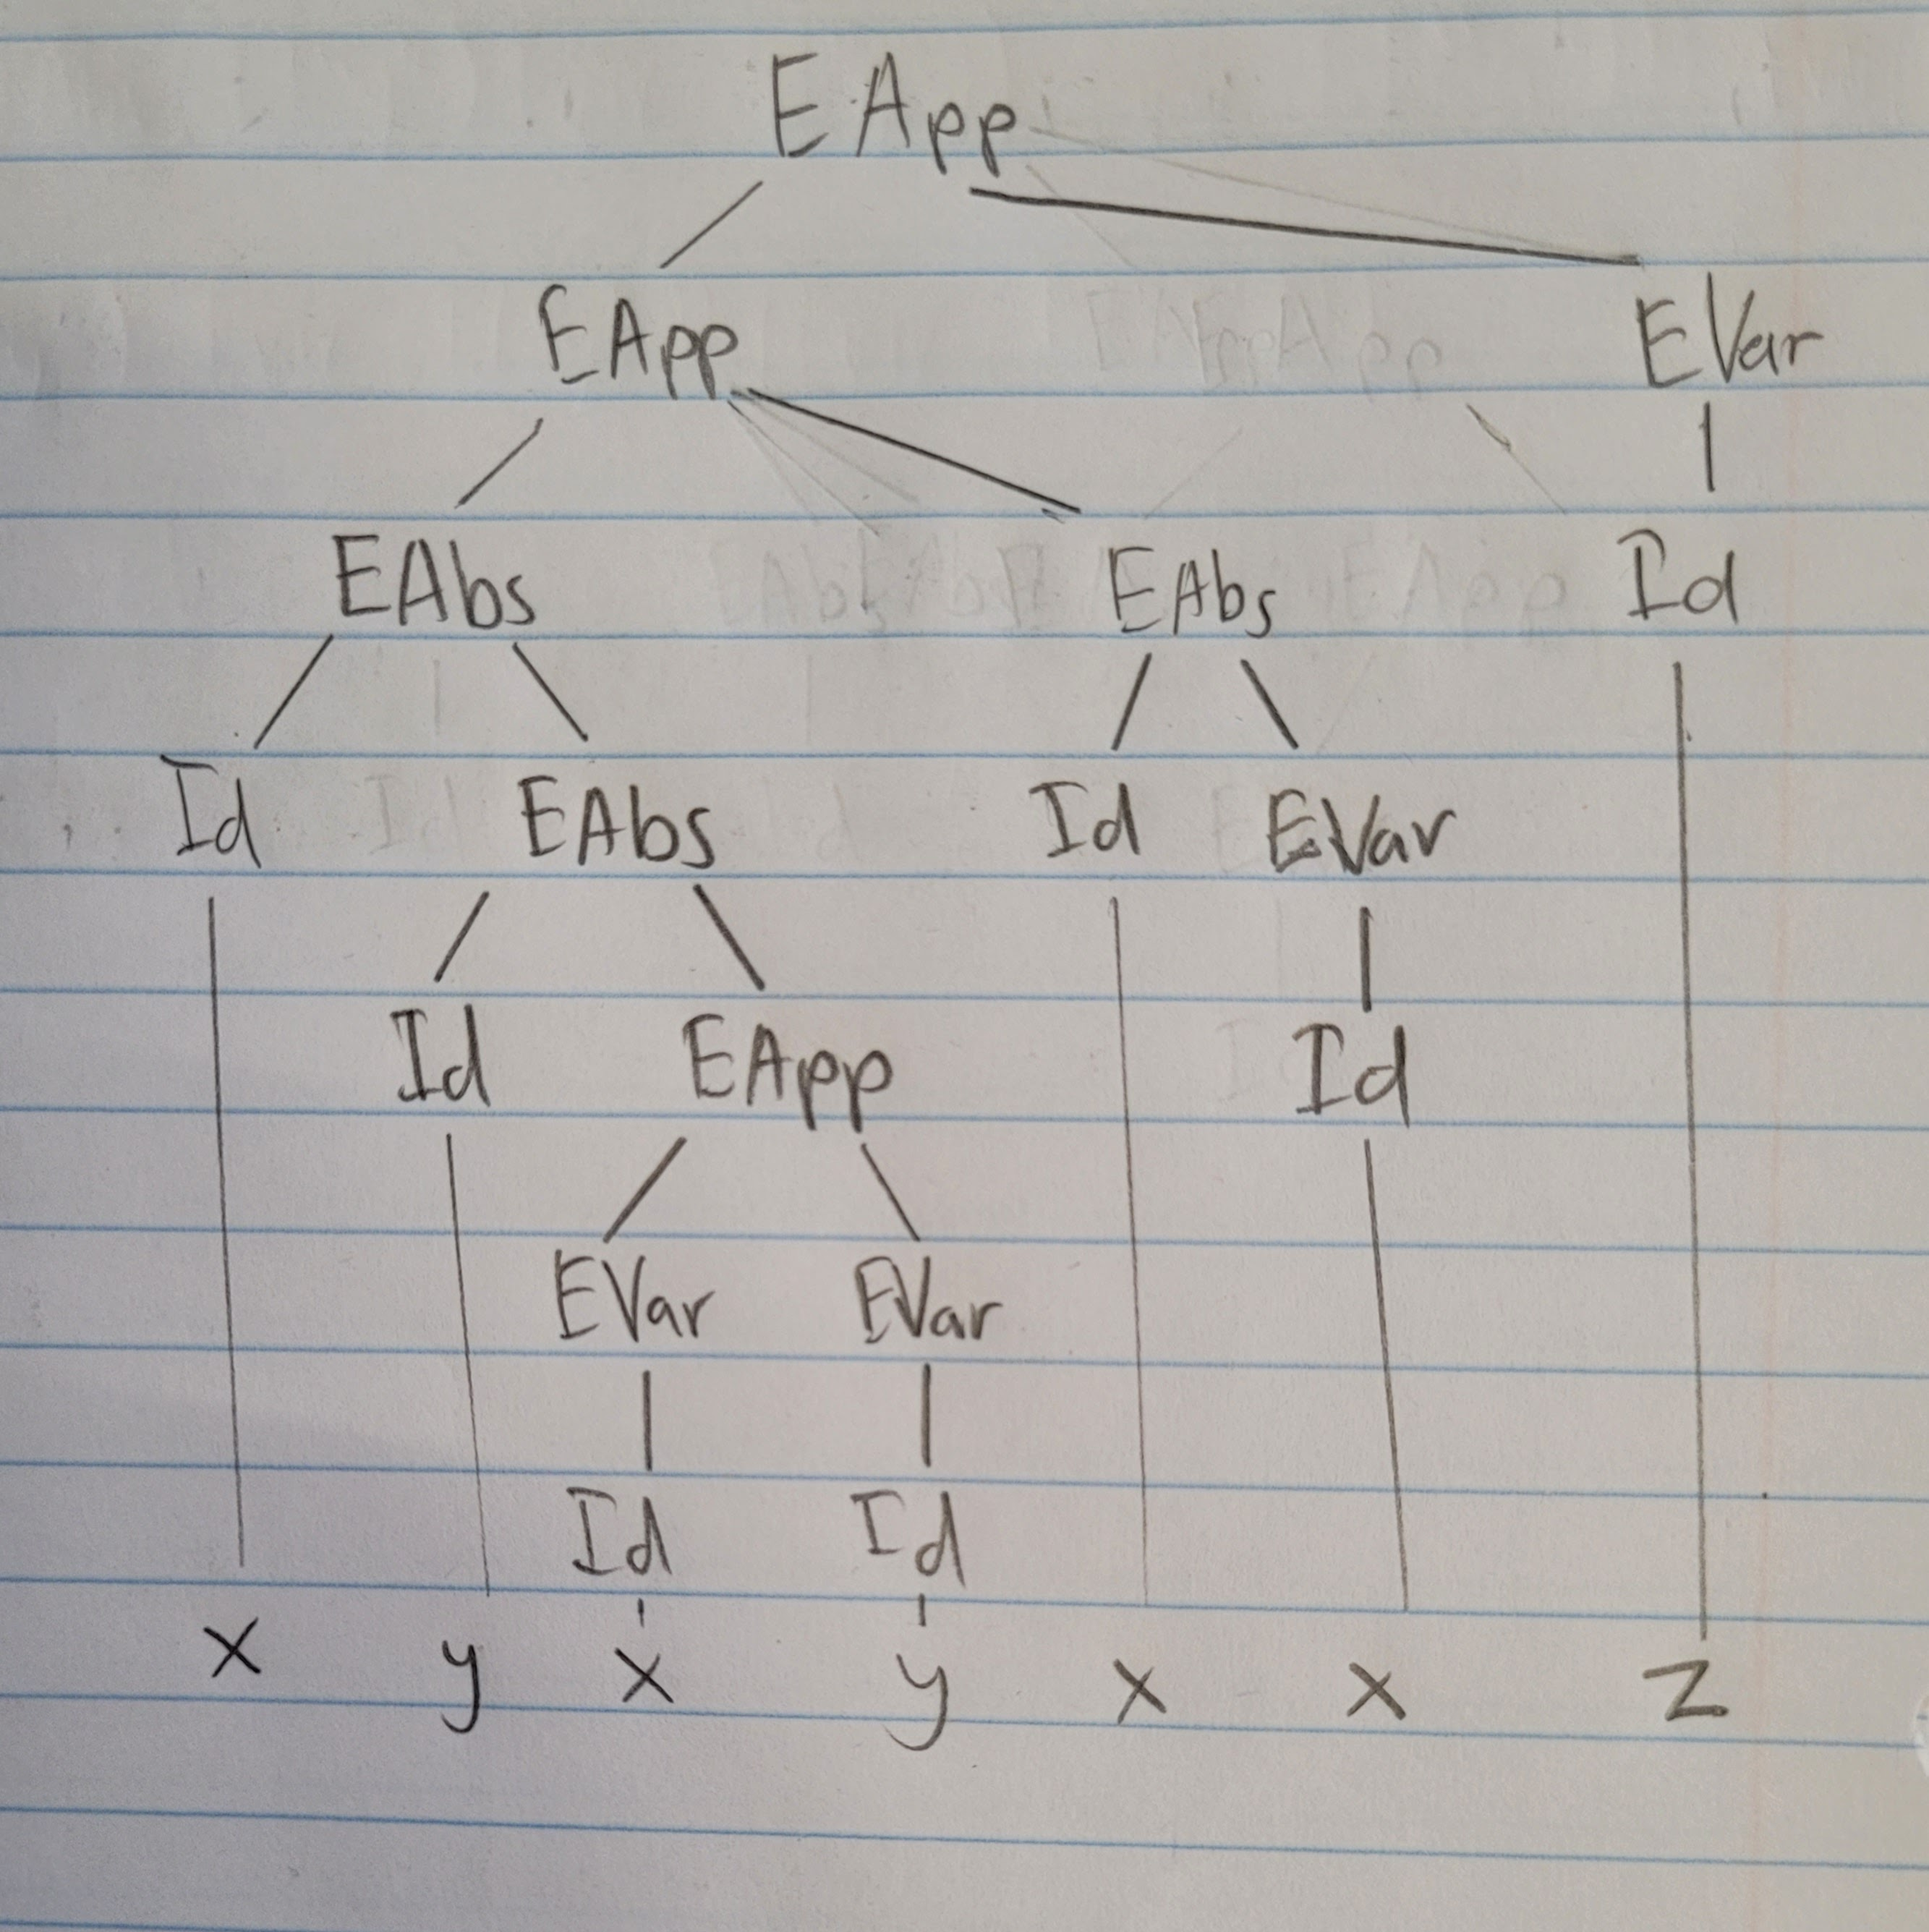
\includegraphics[width=15cm, height=8cm]{Report Images/week5_7.jpg}

The Linearized Tree for (\textbackslash x . \textbackslash y . x y z) a b c is:
\begin{lstlisting}
\ x . \ y . x y z a b c
Prog (EApp (EApp (EApp (EAbs (Id "x") (EAbs (Id "y") (EApp (EApp (EVar (Id "x")) (EVar (Id "y"))) (EVar (Id "z"))))) (EVar (Id "a"))) (EVar (Id "b"))) (EVar (Id "c")))
\end{lstlisting}

Its Abstract Syntax Tree:

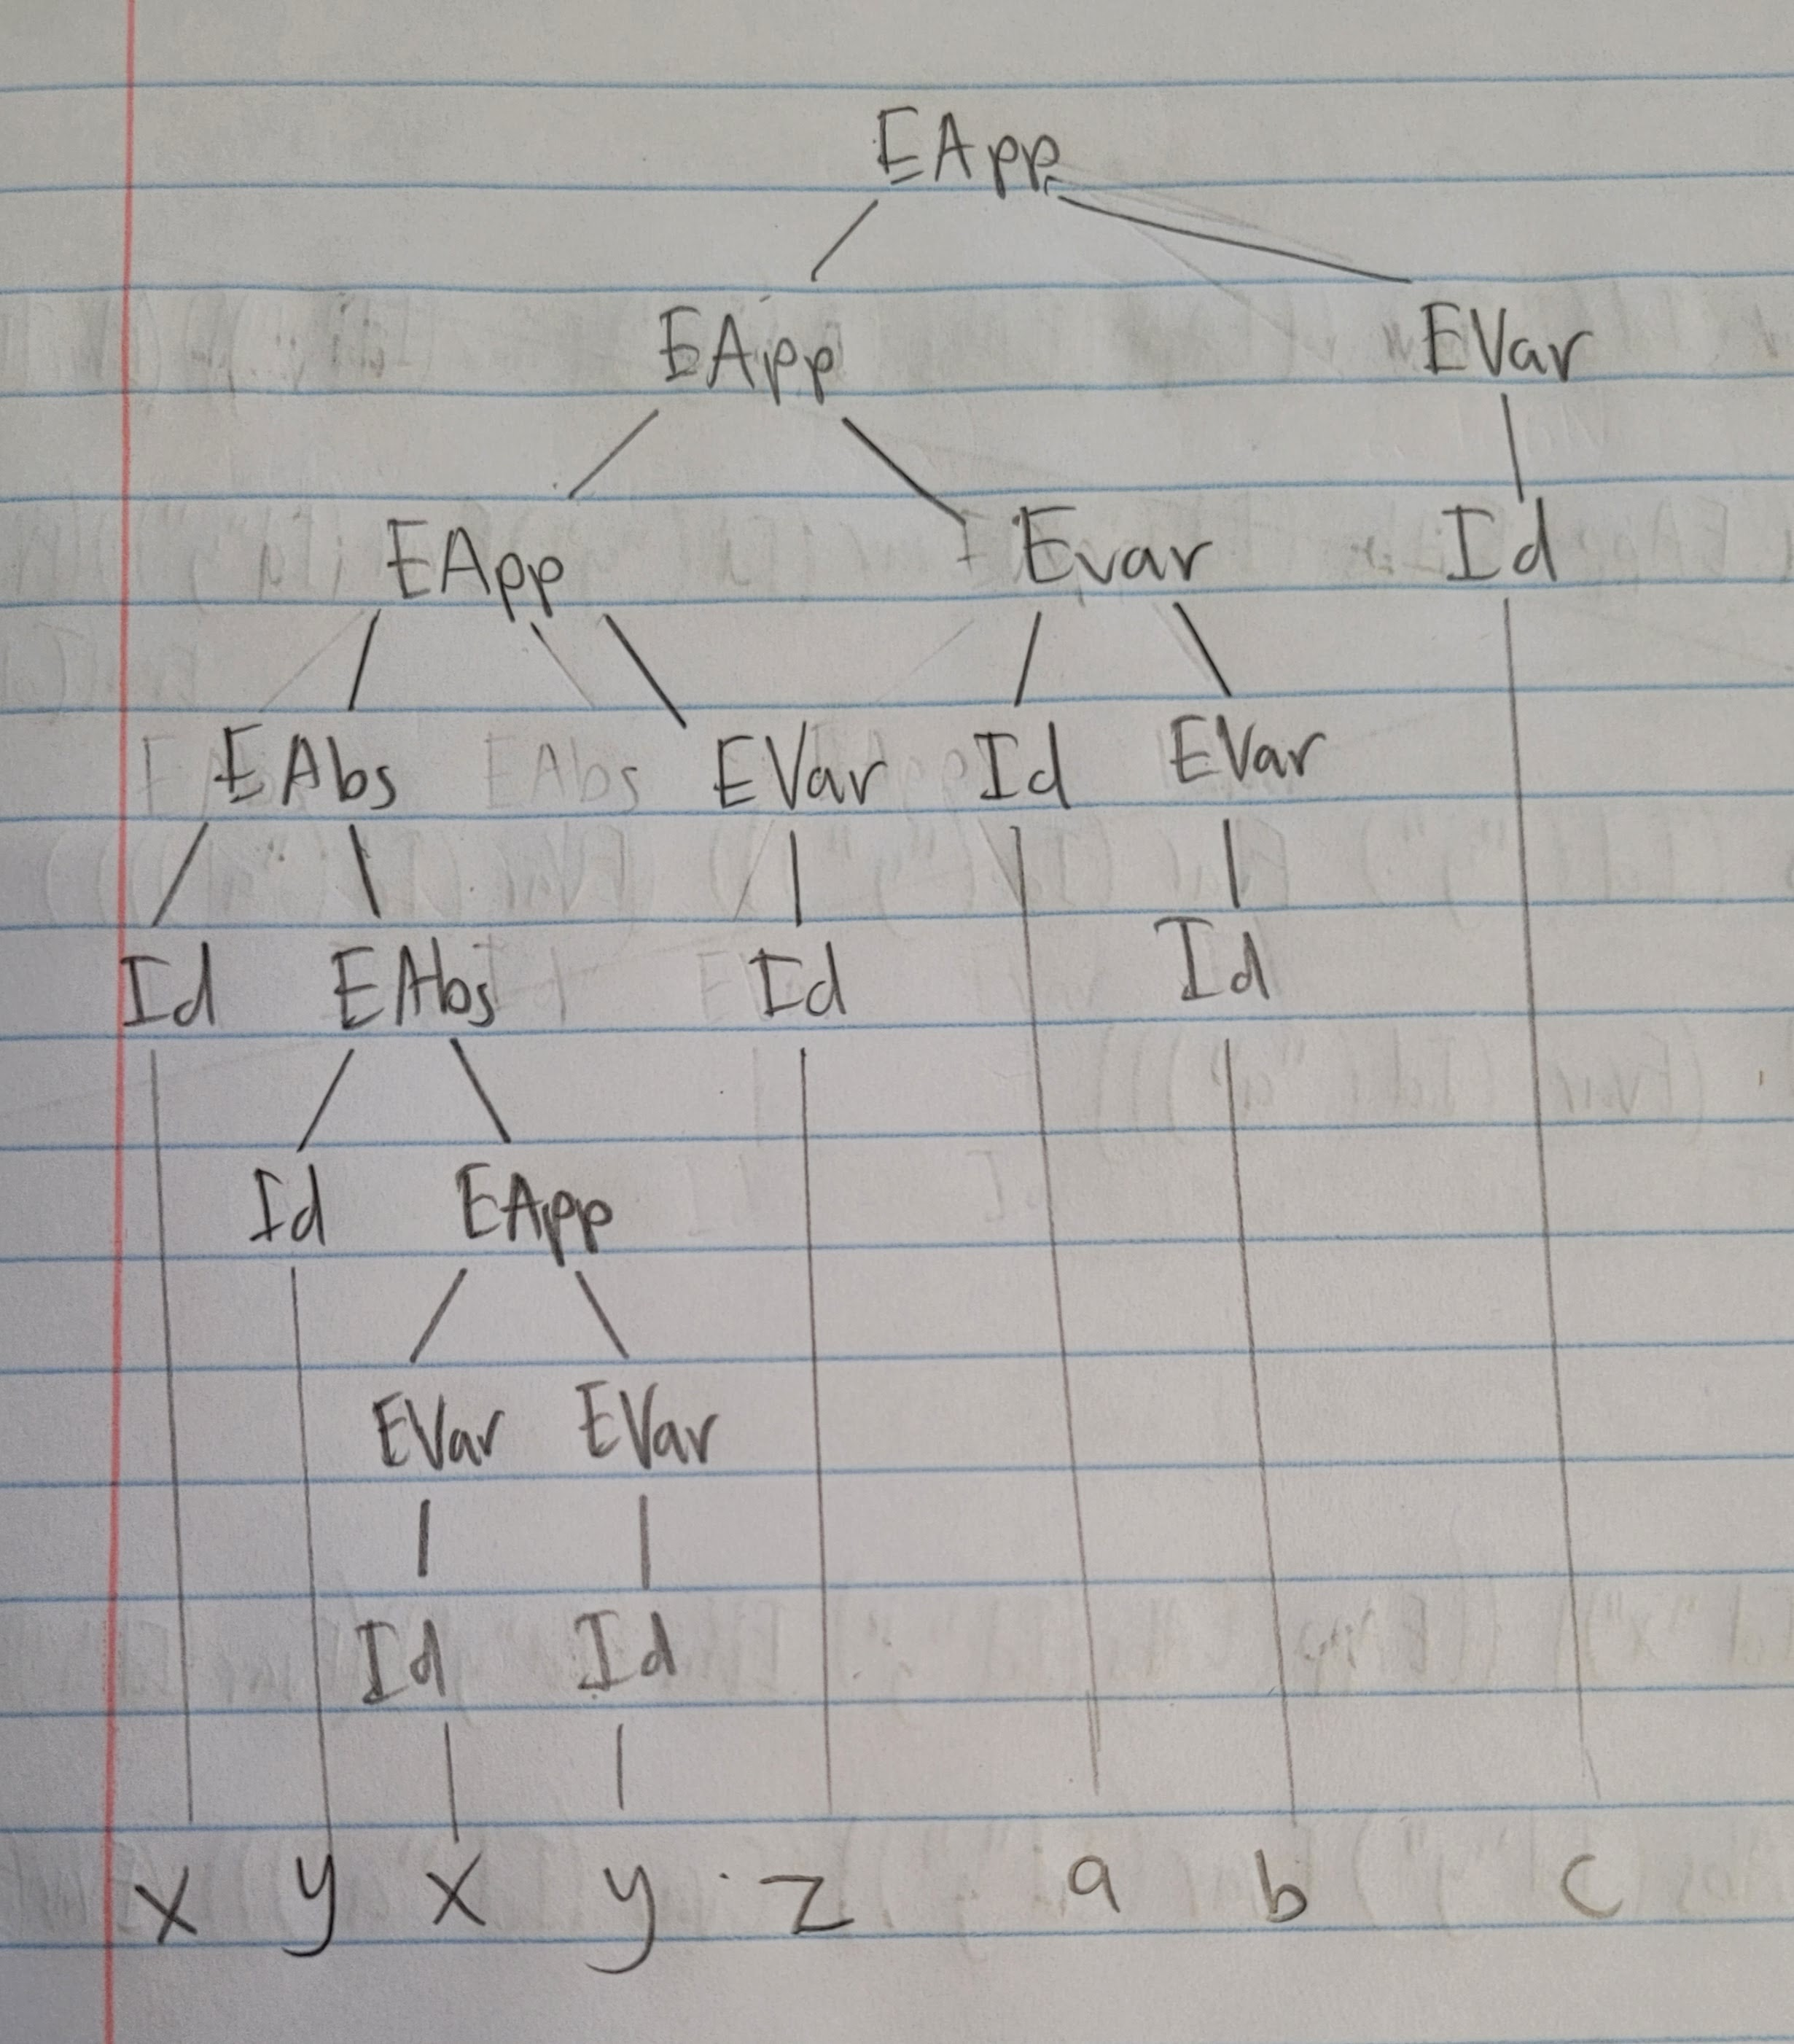
\includegraphics[width=15cm, height=8cm]{Report Images/week5_8.jpg}

\textbf{Part 2:}

Evaluating of Equations:
\begin{lstlisting}
  (\x.x) a = a
  \x.x a = \x.x a
  (\x.\y.x) a b = (\y. a) b = a
  (\x.\y.y) a b = (\y. y) b = b
  (\x.\y.x) a b c = (\y. a) b c = (a) c = a c
  (\x.\y.y) a b c = (\y. y) b c = (b) c = b c
  (\x.\y.x) a (b c) = (\y. a) (b c) = a
  (\x.\y.y) a (b c) = (\y. y) (b c) = b c
  (\x.\y.x) (a b) c = (\y. a b) c = a b
  (\x.\y.y) (a b) c = (\y. y) c = c
  (\x.\y.x) (a b c) = (\y. a b c)
  (\x.\y.y) (a b c) = (\y. y)
\end{lstlisting}

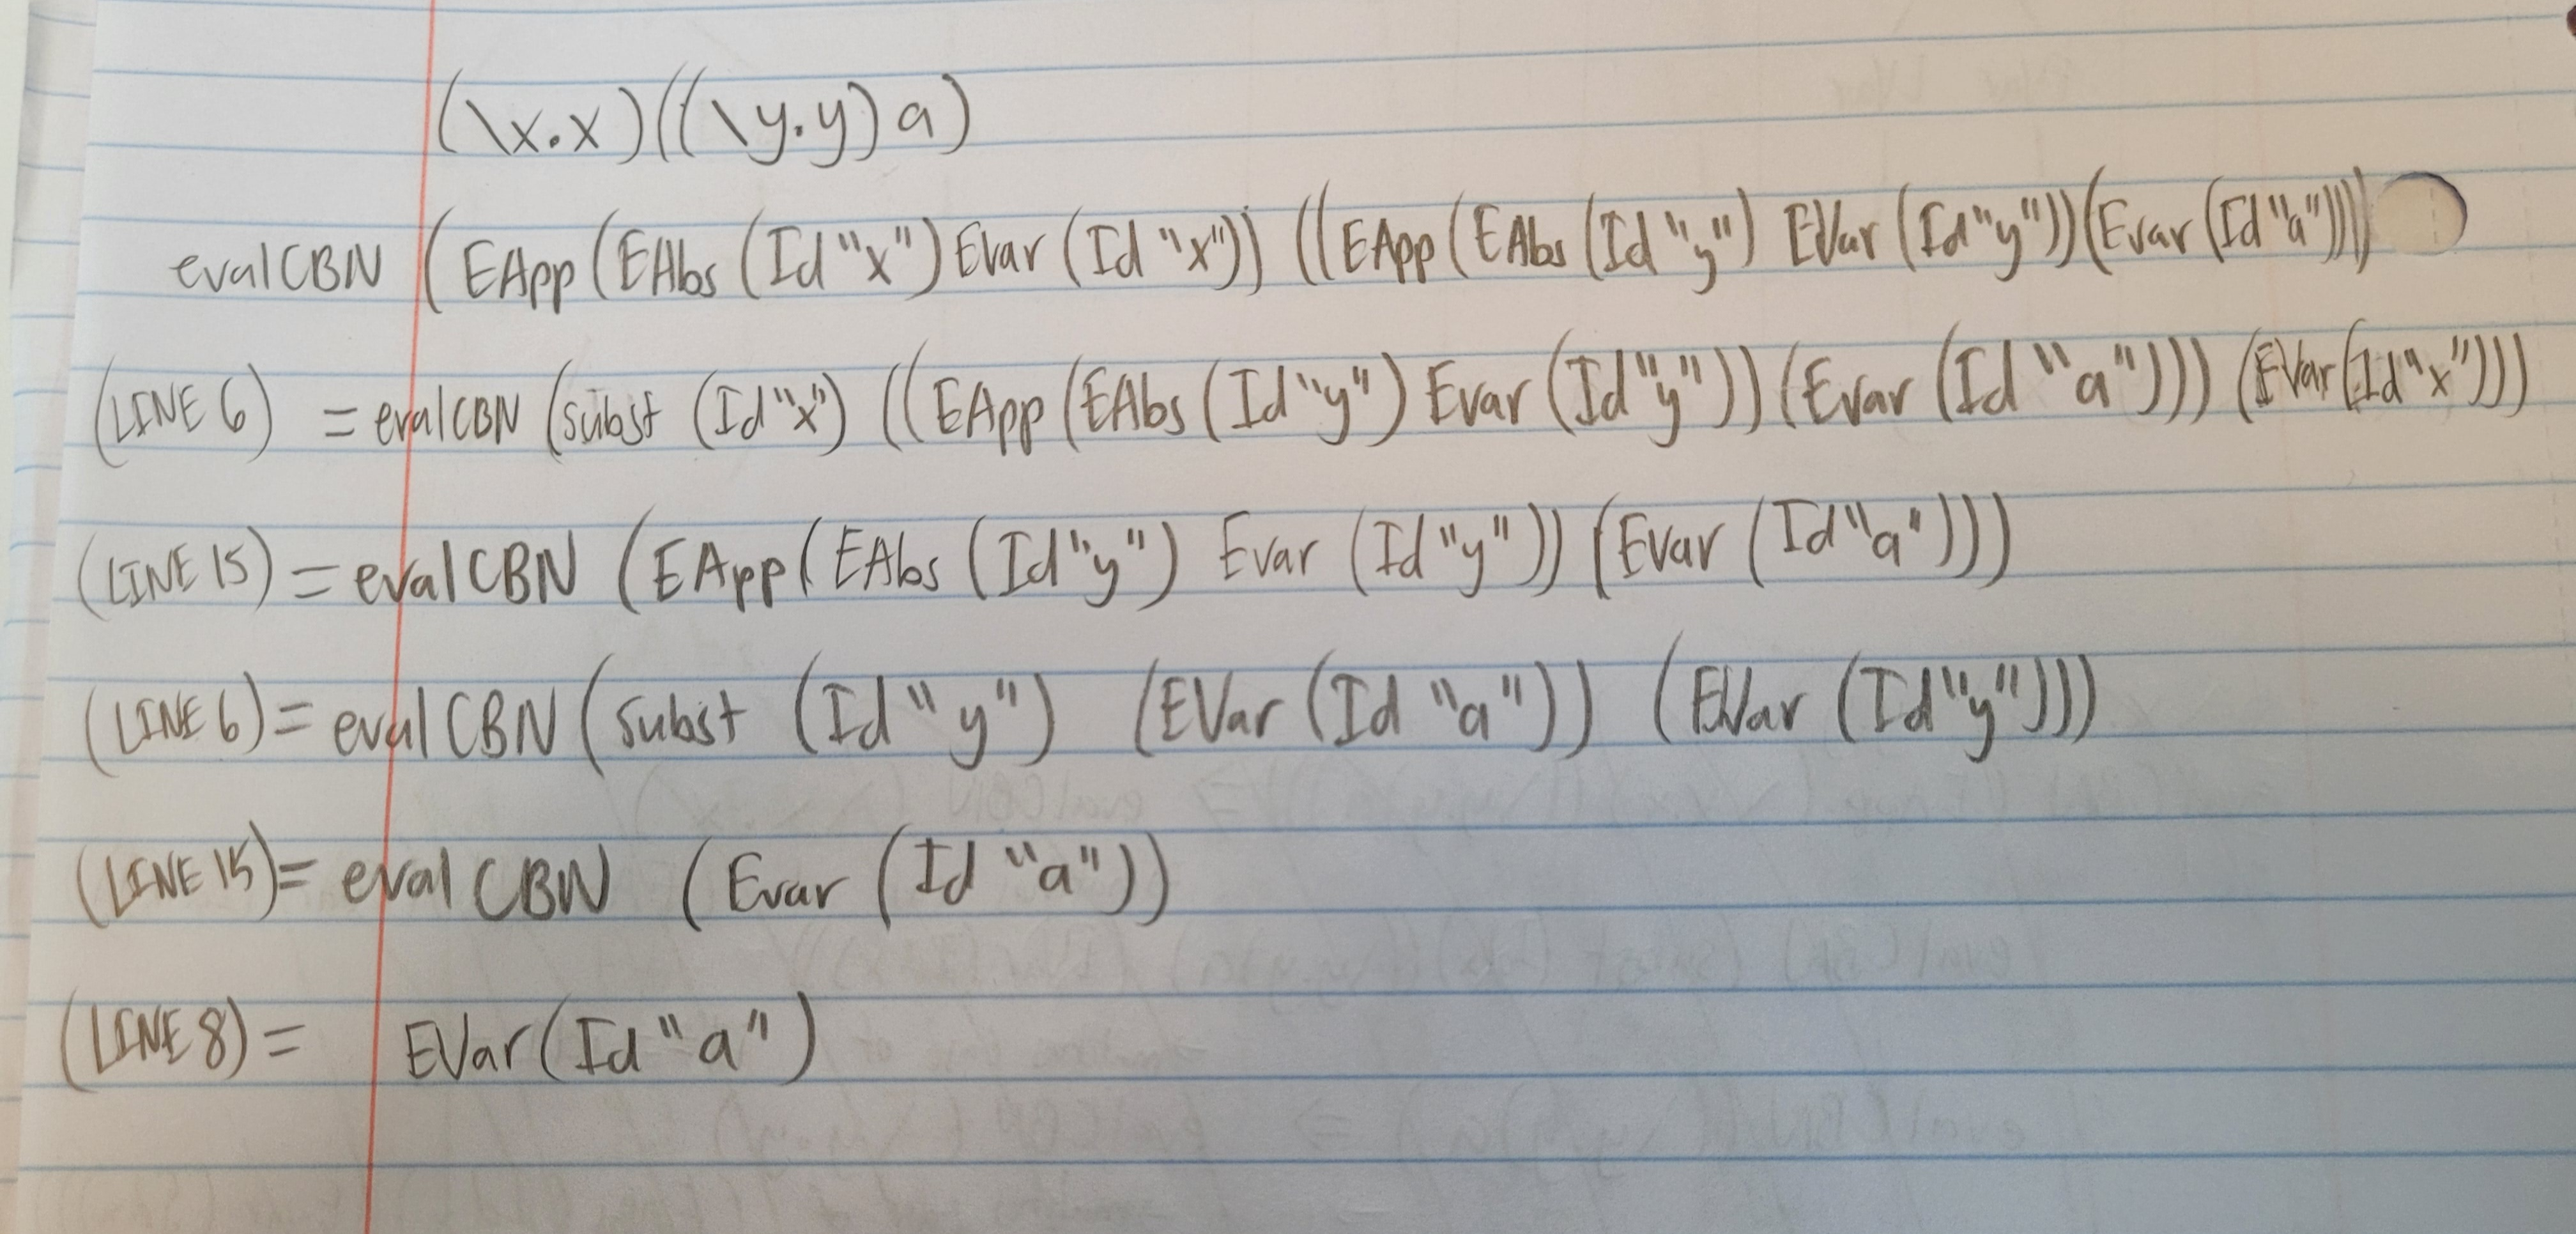
\includegraphics[width=15cm, height=8cm]{Report Images/week5_9.jpg}

\subsection{Week 6}
\begin{lstlisting}
(\exp . \two . \three . exp two three)
(\m.\n. m n)
(\f.\x. f (f x))
(\f.\x. f (f (f x)))

=
((\m.\n. m n) (\f2.\x2. f2 (f2 x2)) (\f3.\x3. f3 (f3 (f3 x3))))
=
((\n. (\f2.\x2. f2 (f2 x2)) n) (\f3.\x3. f3 (f3 (f3 x3))))
=
((\f2.\x2. f2 (f2 x2)) (\f3.\x3. f3 (f3 (f3 x3))))
=
(\x2. (\f3.\x3. f3 (f3 (f3 x3))) ((\f3.\x3. f3 (f3 (f3 x3))) x2))
=
(\x2. (\f3.\x3. f3 (f3 (f3 x3))) (\x3. x2 (x2 (x2 x3))))
=
(\x2. (\x3. (\x3. x2 (x2 (x2 x3))) ((\x3. x2 (x2 (x2 x3))) ((\x3. x2 (x2 (x2 x3))) x3))))
=
(\x2. (\x3. (\x3. x2 (x2 (x2 x3))) ((\x3. x2 (x2 (x2 x3))) ((x2 (x2 (x2 x3)))))))
=
(\x2. (\x3. (\x3. x2 (x2 (x2 x3))) ((x2 (x2 (x2 (x2 (x2 (x2 x3)))))))))
=
(\x2. (\x3. (x2 (x2 (x2 (x2 (x2 (x2 (x2 (x2 (x2 x3)))))))))))
\end{lstlisting}
\subsection{Week 7}

For lines 5-8 as shown through:
\begin{lstlisting}
evalCBN (EApp e1 e2) = case (evalCBN e1) of
    (EAbs i e3) -> evalCBN (subst i e2 e3)
    e3 -> EApp e3 e2
evalCBN x = x
\end{lstlisting}
In \textit{Line 5}, \textit{e1} and \textit{e2} are bound to the left of \textit{=}, and the scope is the end of \textit{Line 7}. For \textit{Line 6}, the variables \textit{i} and \textit{e3} are bound to the left of \textit{->}, and the scope is the end of the same line. Meanwhile, in \textit{Line 7}, the variable \textit{e3} is bound to the left of \textit{->}, and its scope is the end of the same line. Finally, for \textit{Line 8}, the variable \textit{x} is bound to the left of \textit{=}, and its scope is the end of the same line.
\\
\\
For lines 18-22 as shown through:
\begin{lstlisting}
subst id s (EAbs id1 e1) =
    -- to avoid variable capture, we first substitute id1 with a fresh name inside the body of the Lambda-abstraction, obtaining e2. Only then do we proceed to apply substitution of the original s for id in the body e2.
    let f = fresh (EAbs id1 e1)
        e2 = subst id1 (EVar f) e1 in
        EAbs f (subst id s e2)
\end{lstlisting}
In \textit{Line 18}, the variables \textit{id}, \textit{s}, \textit{id1}, and \textit{e1} are all bound to the left of \textit{=}, and the scope is the end of \textit{Line 22}. Meanwhile, in \textit{Line 20}, the variable \textit{f} is bound to the left of \textit{=}, and the scope is also the end of \textit{Line 22}. Lastly, on \textit{Line 21}, the variable \textit{e2} is bound by \textit{=}, and its scope is the end of \textit{Line 22} as well.
\\
\\
Item 3:
\begin{lstlisting}
--Idea:
(\x.\y.x) y z = (\fresh.y) z = y

(EApp (EApp (EAbs (Id "x") (EAbs (Id "y") (EVar (Id "x")))) (EVar (Id "y"))) (EVar (Id "z")))

-- In first EApp, (EApp (EAbs (Id "x") (EAbs (Id "y") (EVar (Id "x")))) (EVar (Id "y"))) is e1, (EVar (Id "z")) is e2
-- In second EApp, (EAbs (Id "x") (EAbs (Id "y") (EVar (Id "x")))) is e1, (EVar (Id "y")) is e2

= -- Line 5
evalCBN ( ( evalCBN (EApp (EAbs (Id "x") (EAbs (Id "y") (EVar (Id "x")))) (EVar (Id "y"))) ) (EVar (Id "z")) )

    -- inner evalCBN
    -- Line 6
    evalCBN (subst ((EAbs (Id "x")) (EVar (Id "y")) (EAbs (Id "y") (EVar (Id "x")))))

        -- Line 18
        -- Line 20
        f = fresh ((EAbs (Id "y") (EVar (Id "x"))))
        -- consider \y now \y0
        -- Line 21
        e2 = subst (Id "y") (EVar "y0") (EVar (Id "x"))
        -- Line 16
        EAbs (Id "y0") (subst (Id "y") (EVar (Id "y")) (EVar (Id "x")))
        -- Line 16

    evalCBN (EAbs (Id "y0") (EVar (Id "y")))

= -- Line 7
evalCBN (EApp (EAbs (Id "y0")) (EVar (Id "y"))) (EVar (Id "z"))
= -- Line 6
evalCBN (subst (Id "y0") (EVar (Id "z")) (EVar (Id "y")))
= -- Line 16
evalCBN (EVar (Id "y"))
= -- Line 8
EVar (Id "y")
\end{lstlisting}
1. \textit{A = \{ \}}
\\ 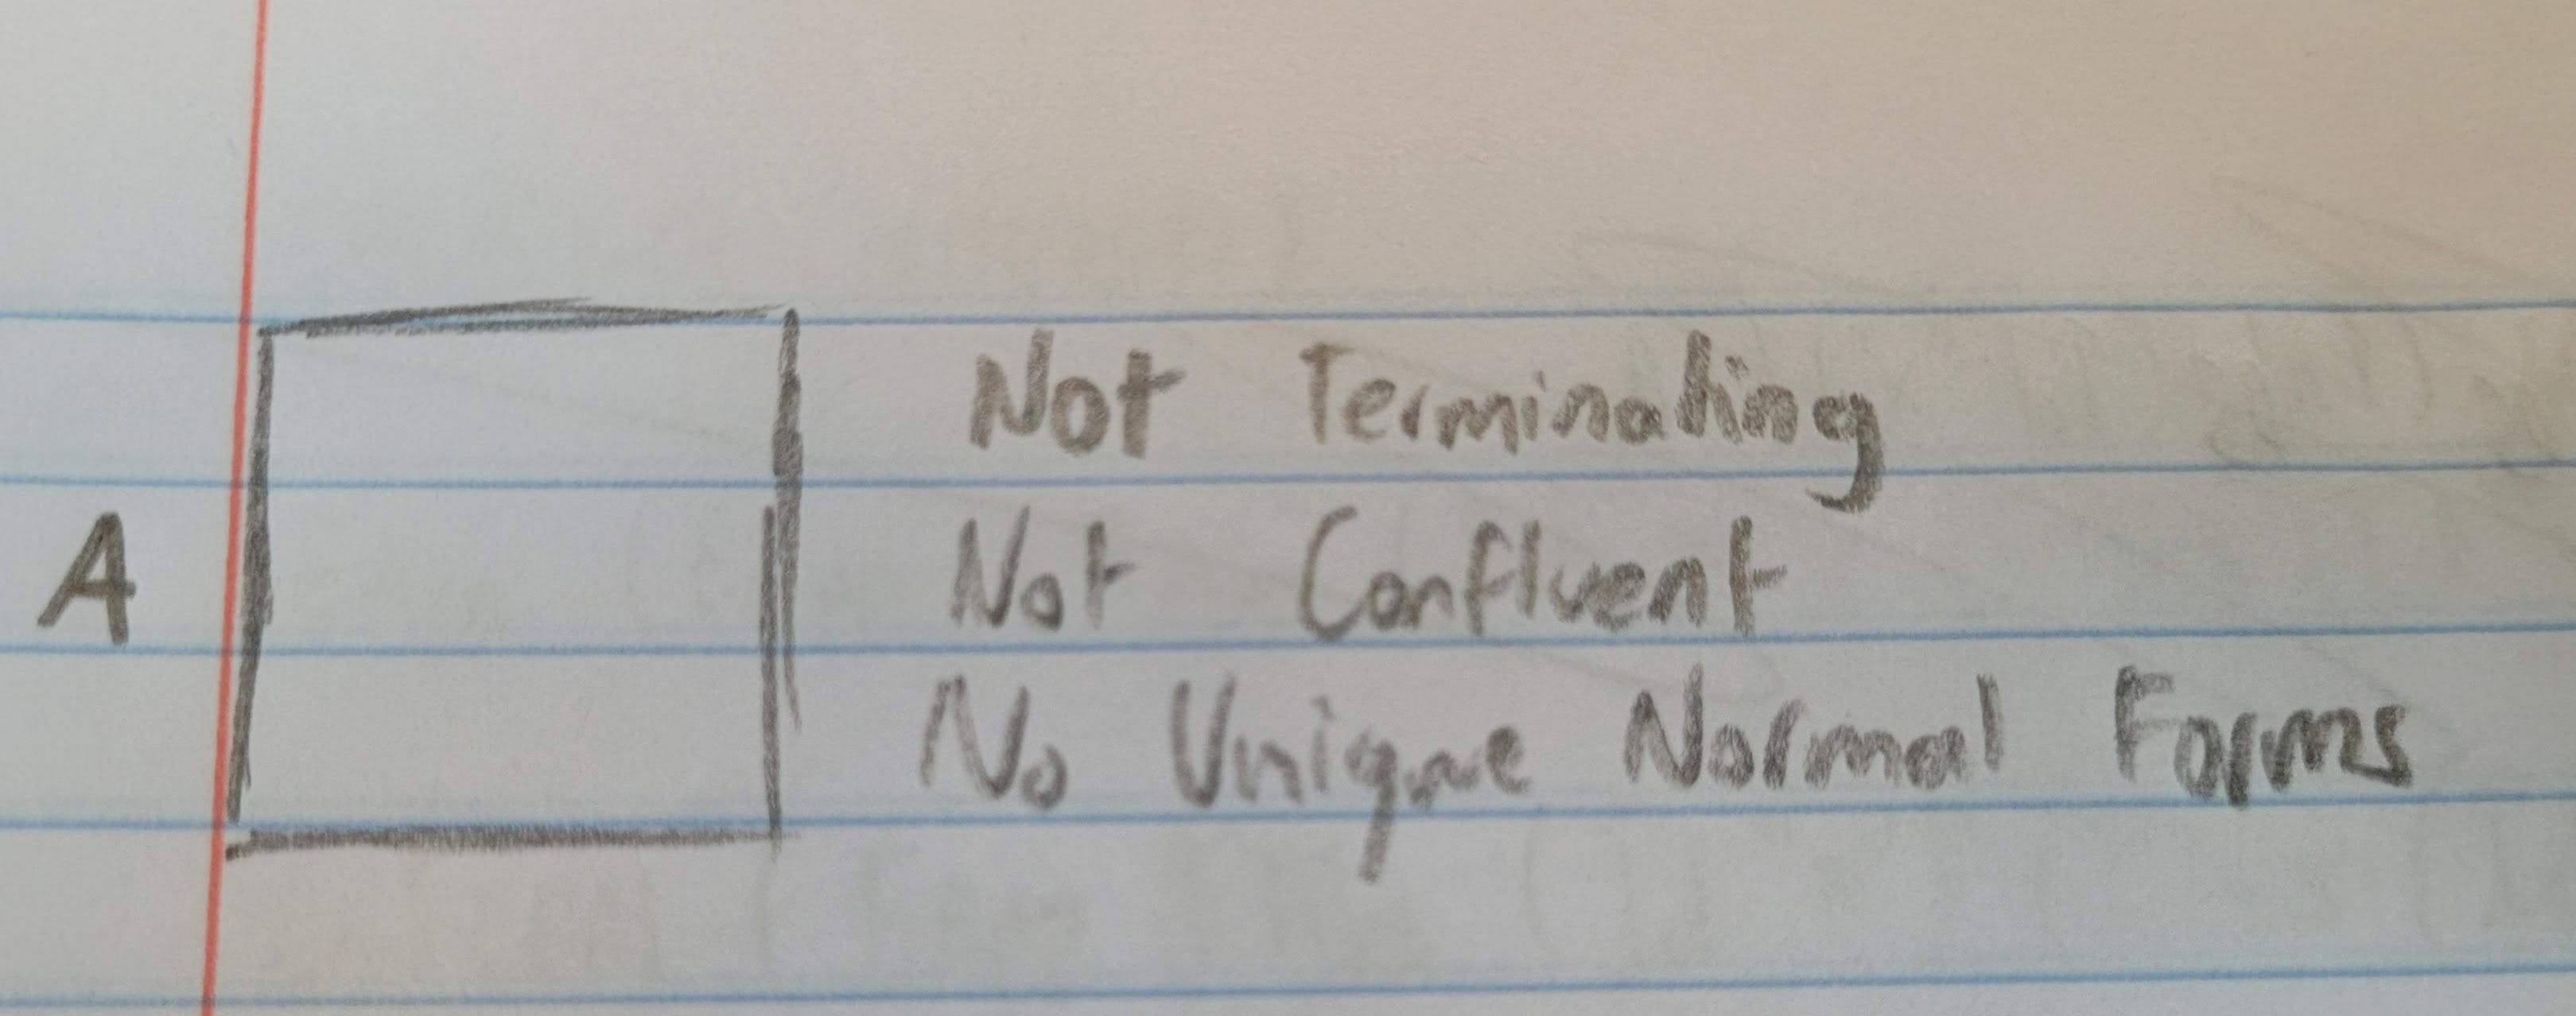
\includegraphics[width=15cm, height=8cm]{Report Images/week7_1.jpg}
\\2. \textit{A = \{a\}} and \textit{R = \{\}}
\\ 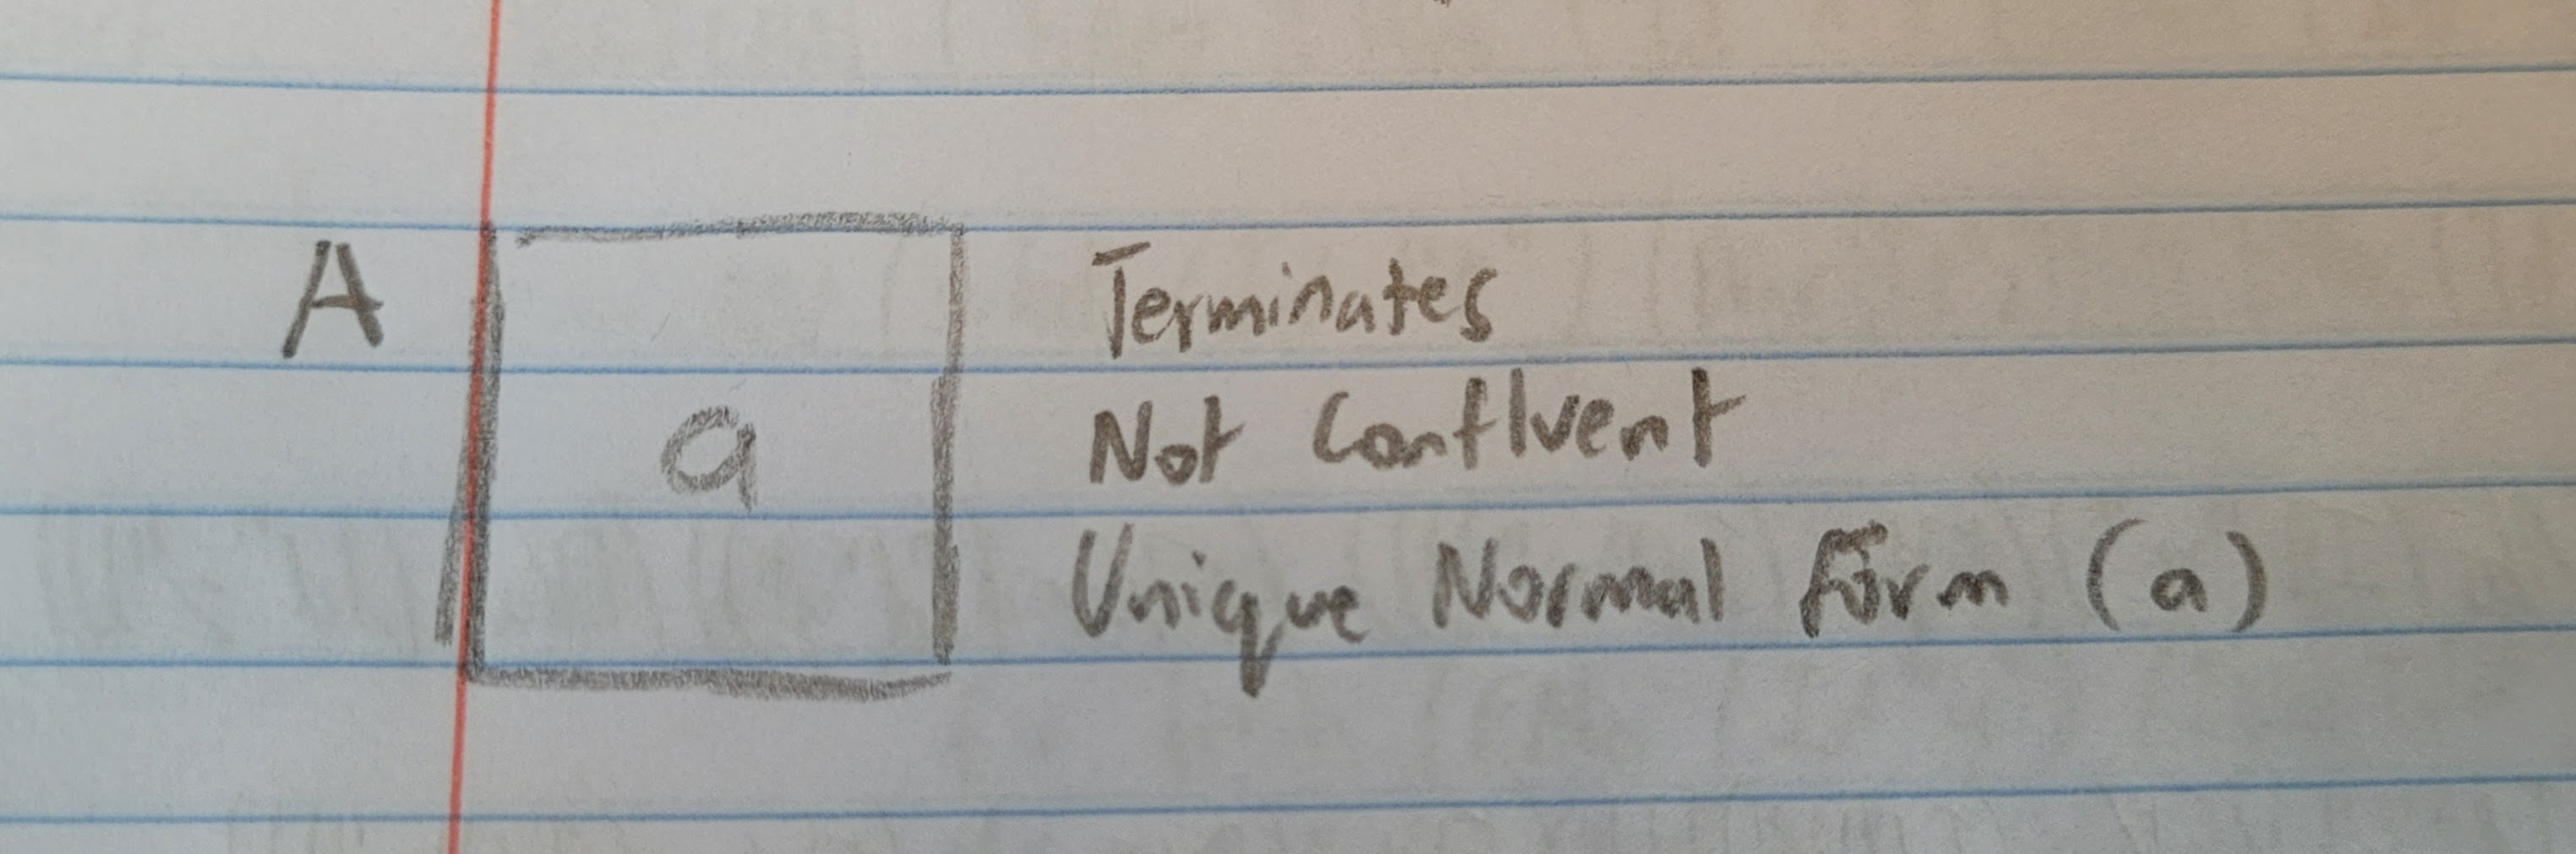
\includegraphics[width=15cm, height=8cm]{Report Images/week7_2.jpg}
\\3. \textit{A = \{a\}} and \textit{R = \{(a,a)\}}
\\ 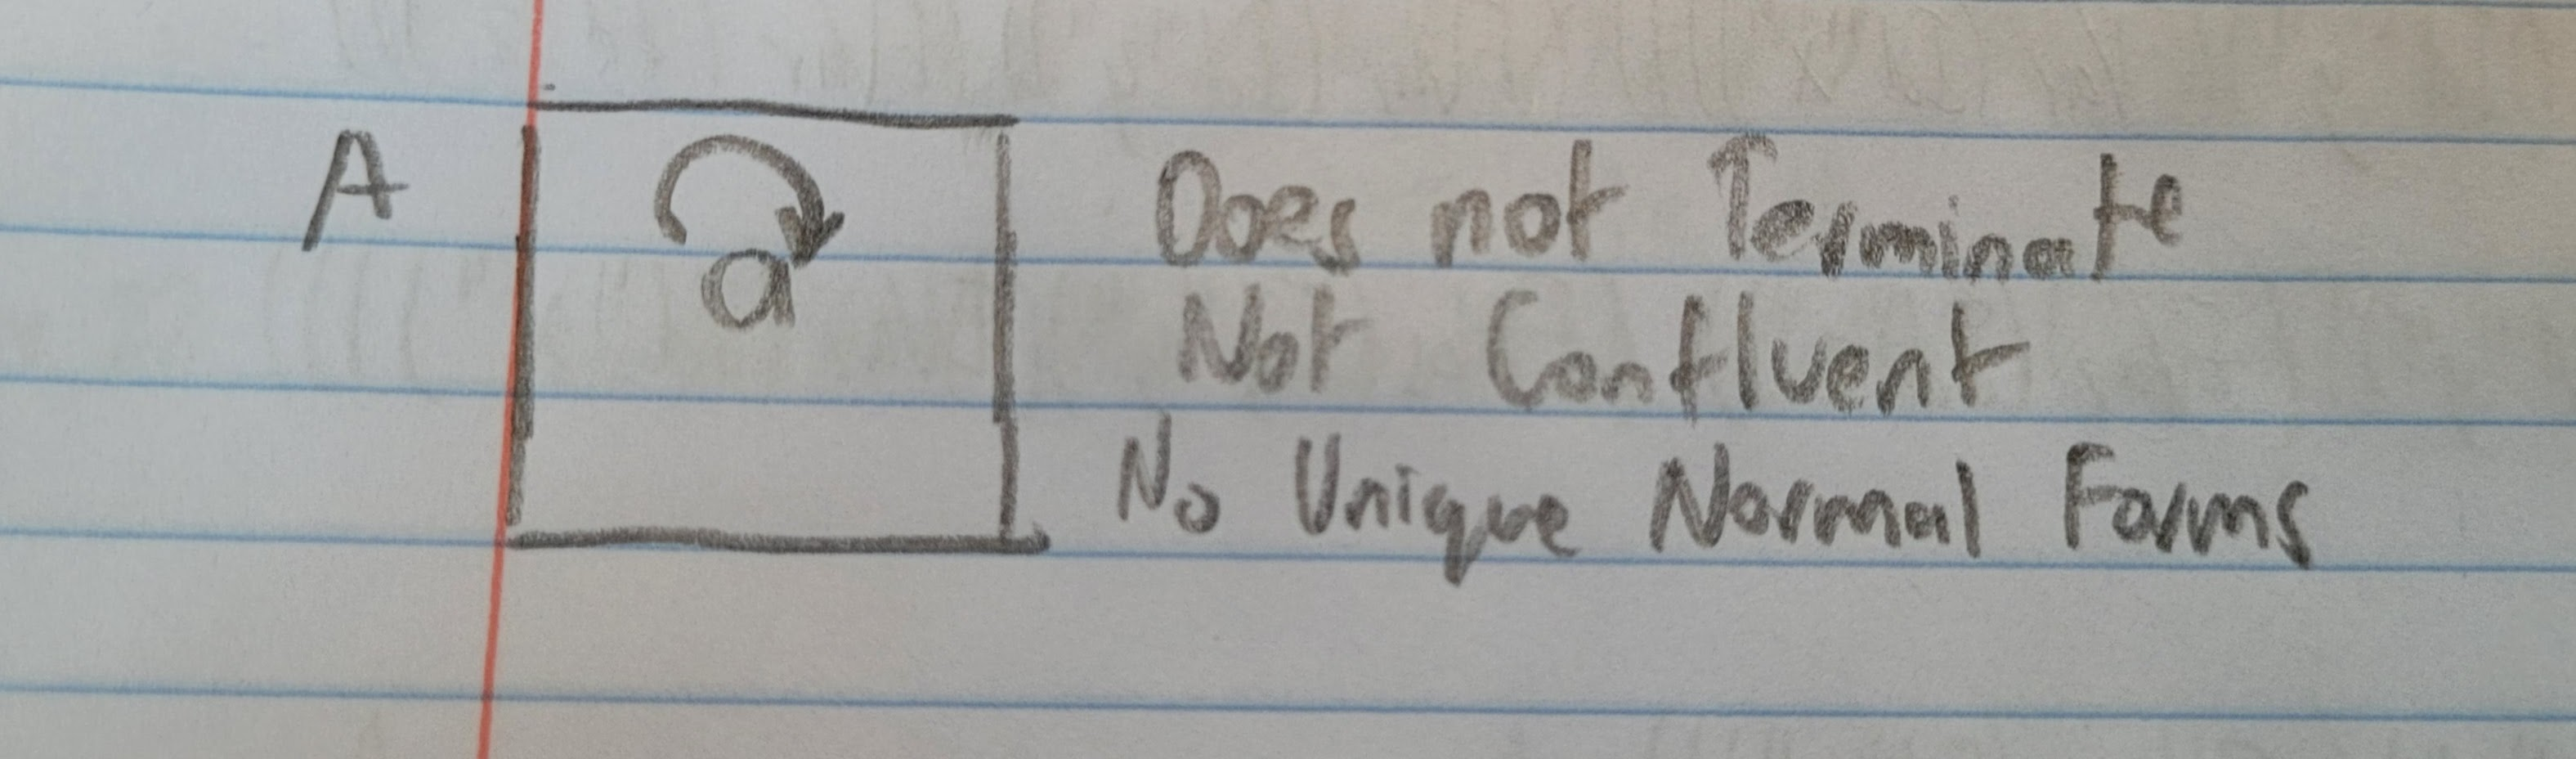
\includegraphics[width=15cm, height=8cm]{Report Images/week7_3.jpg}
\\4. \textit{A = \{a, b, c\}} and \textit{R = \{(a,b), (a,c)\}}
\\ 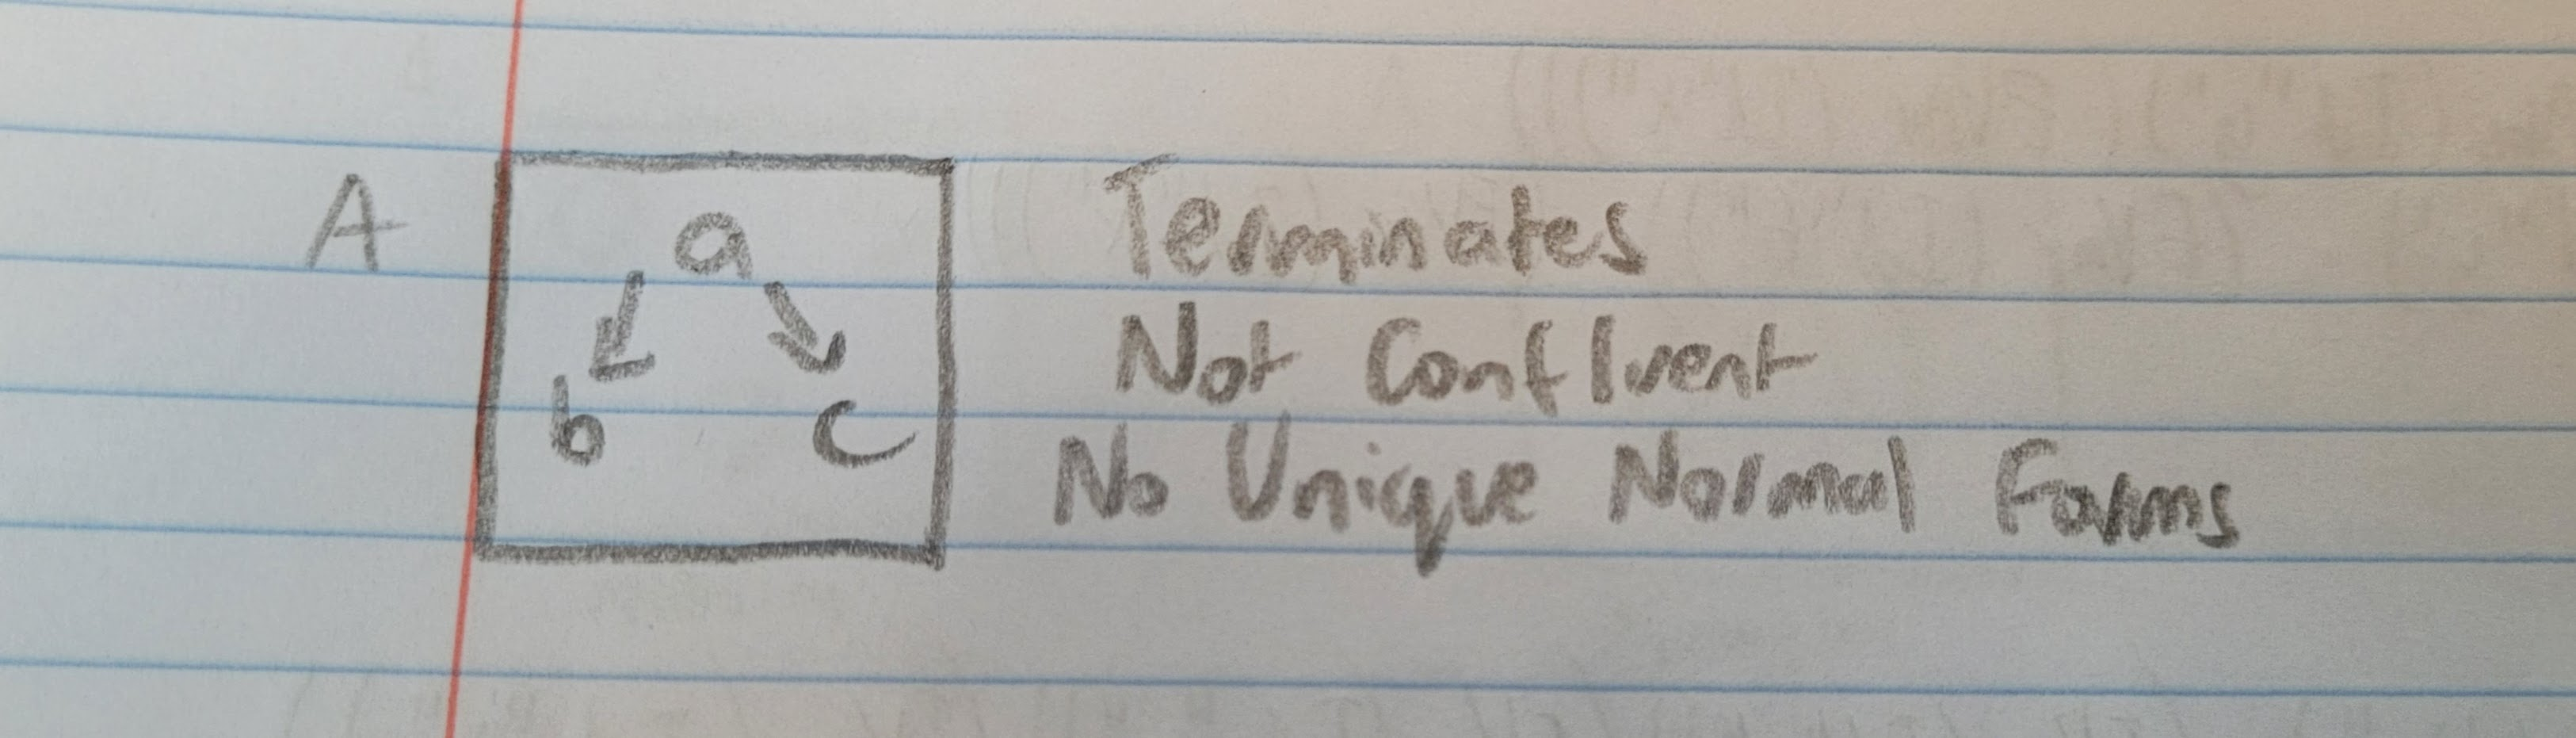
\includegraphics[width=15cm, height=8cm]{Report Images/week7_4.jpg}
\\5. \textit{A = \{a,b\}} and \textit{R = \{(a,a),(a,b)\}}
\\ 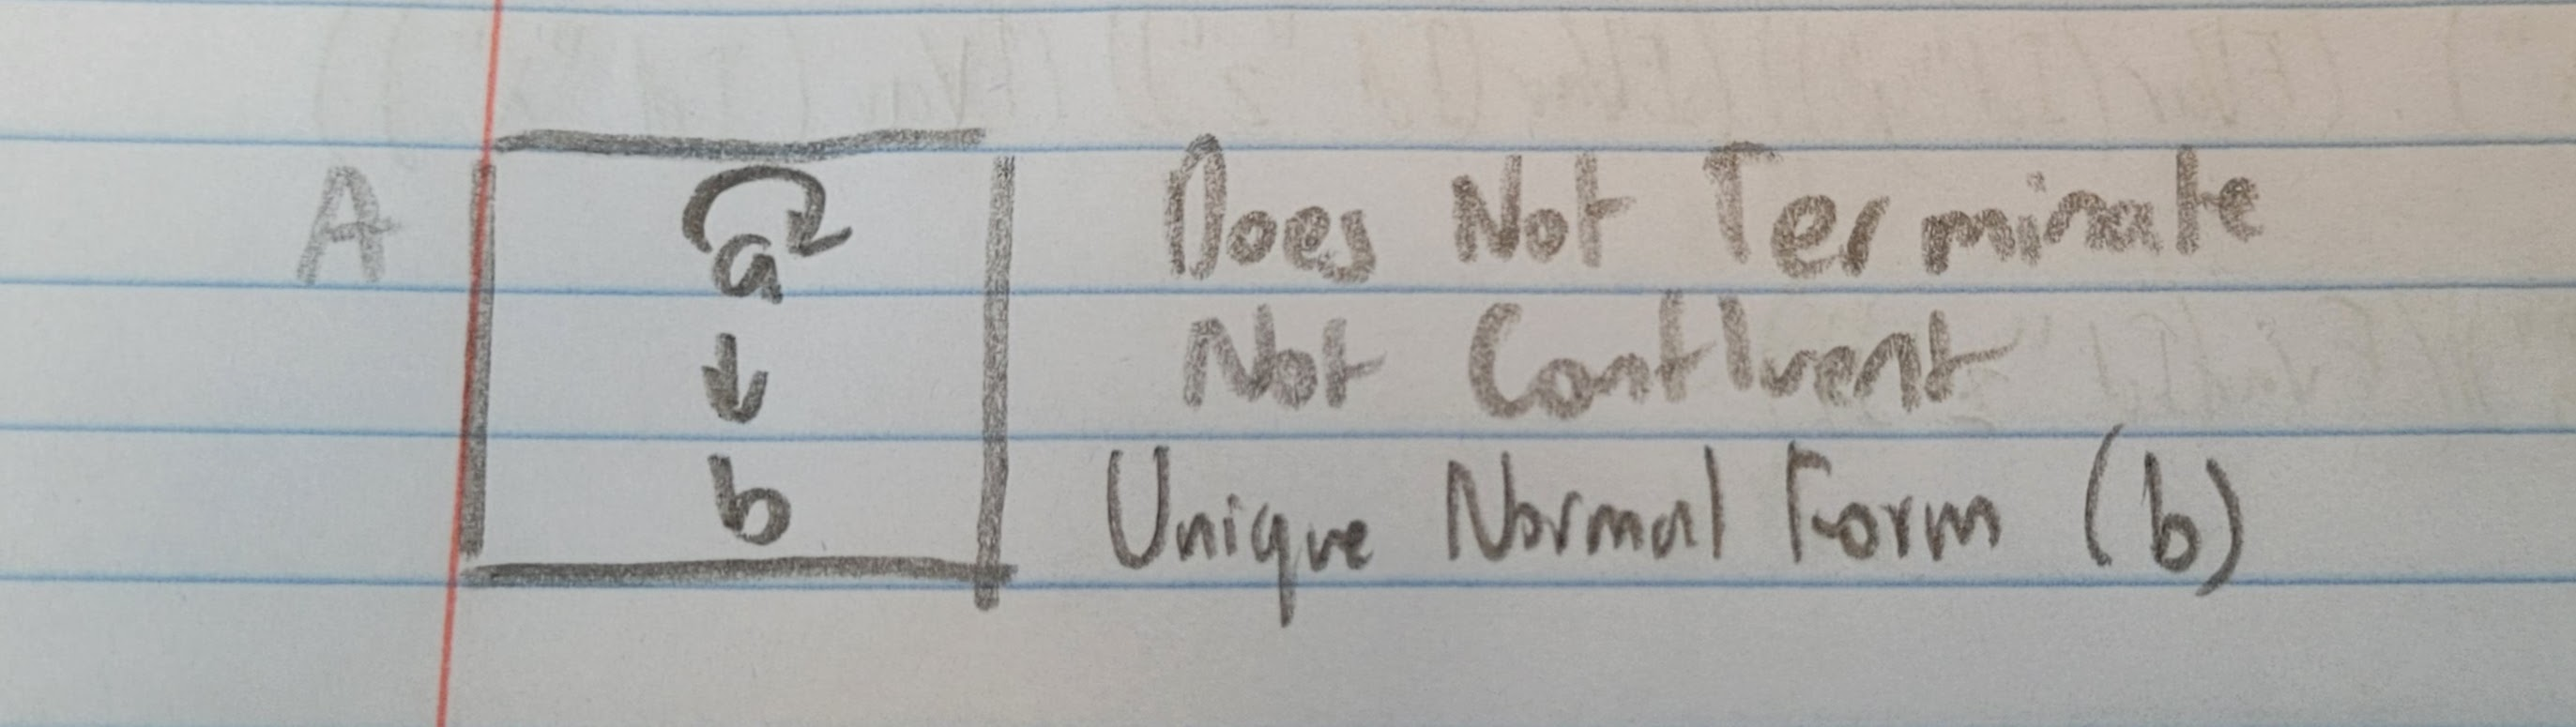
\includegraphics[width=15cm, height=8cm]{Report Images/week7_5.jpg}
\\6. \textit{A = \{a, b, c\}} and \textit{R = \{(a,b),(b,b),(a,c)\}}
\\ 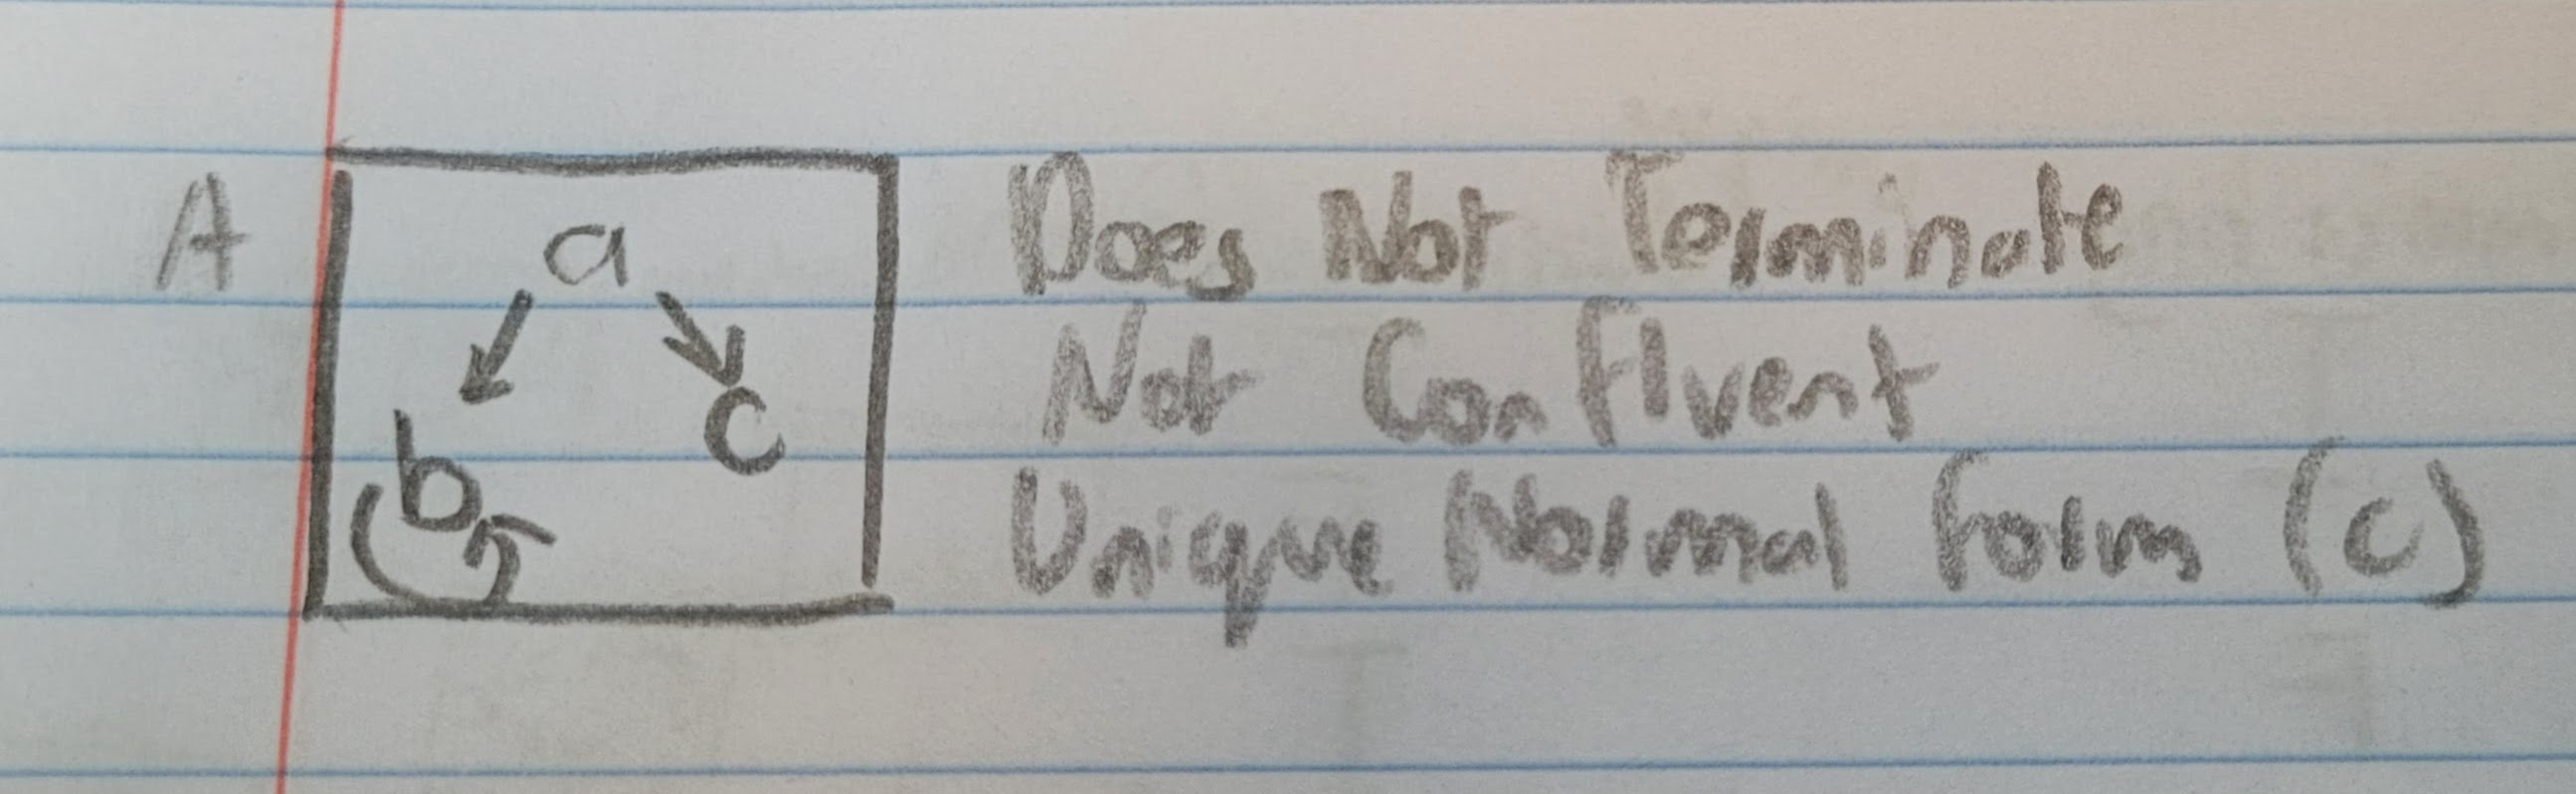
\includegraphics[width=15cm, height=8cm]{Report Images/week7_6.jpg}
\\7. \textit{A = \{a, b, c\}} and \textit{R = \{(a,b),(b,b),(a,c),(c,c)\}}
\\ 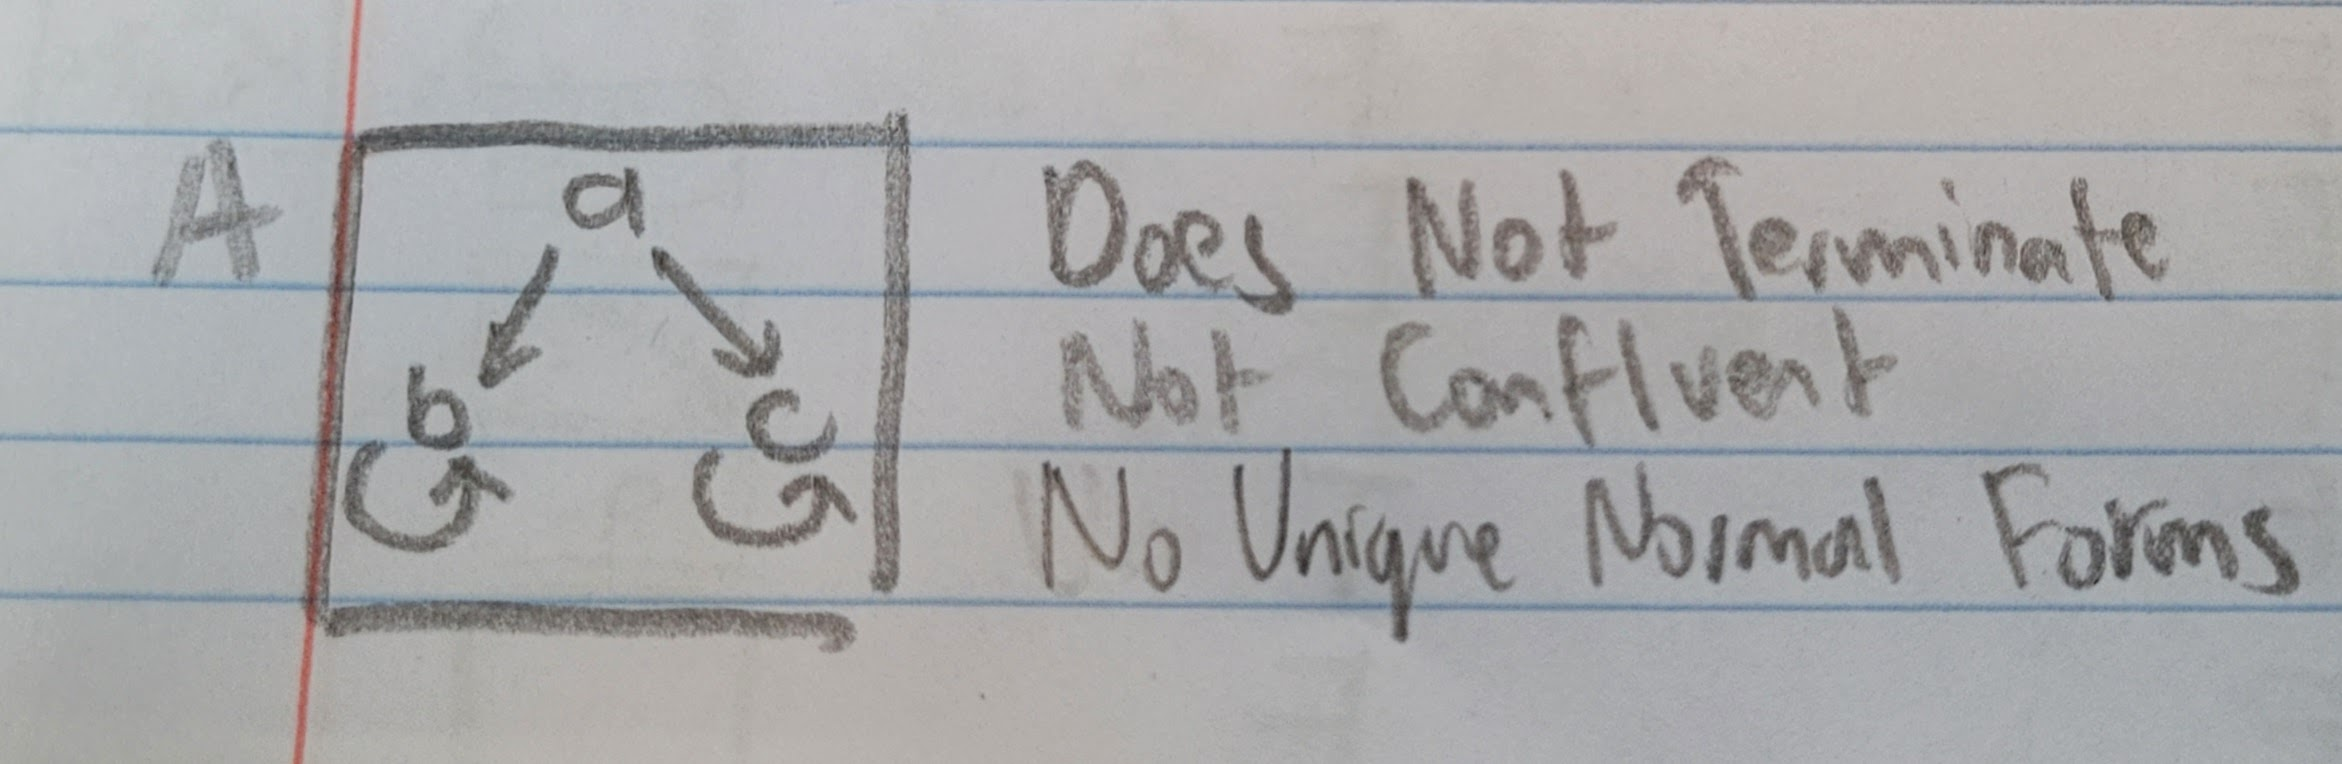
\includegraphics[width=15cm, height=8cm]{Report Images/week7_7.jpg}
\\
\\Example for cases
\\ 1. Confluent: True, Terminating: True, Unique Normal Forms: True
\\ 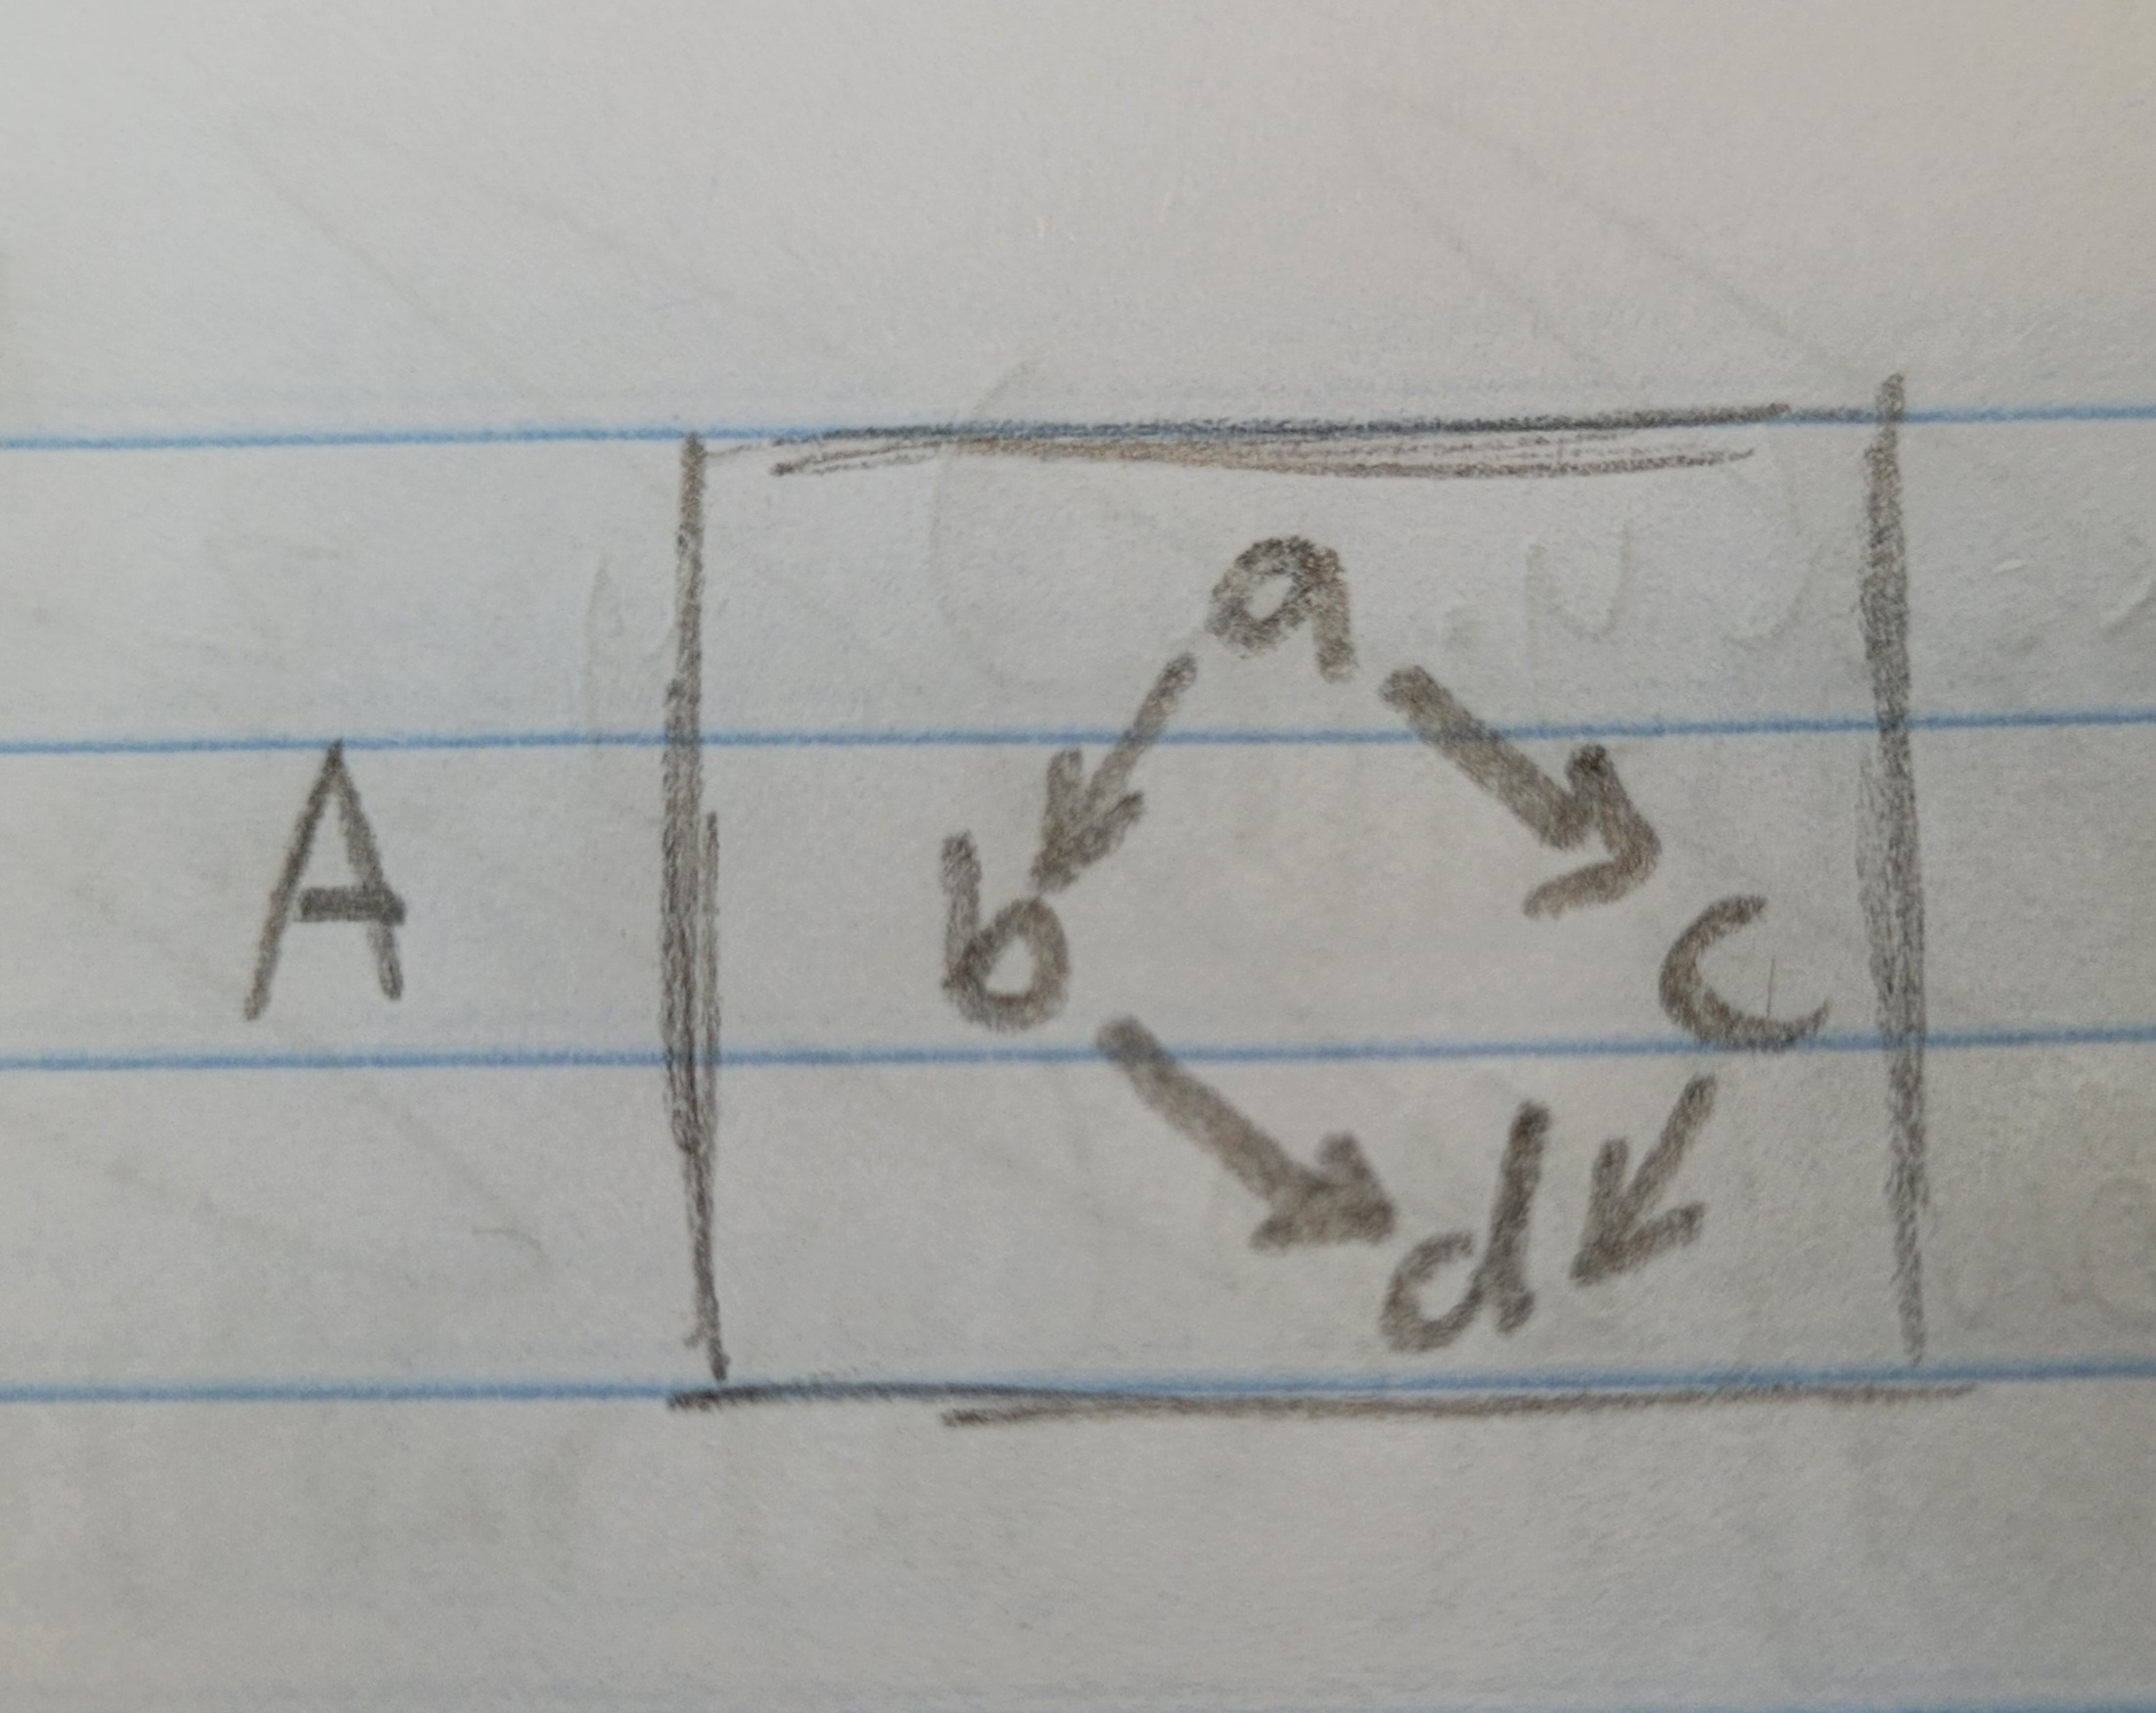
\includegraphics[width=15cm, height=8cm]{Report Images/week7_8.jpg}
\\ 2. Confluent: True, Terminating: True, Unique Normal Forms: False
\\  No example of this would exist, as in order for an ARS to be Terminating and Confluent it would need an Unique Normal Form as if one of the normal forms of the initial term reduces to itself, while the other normal form reduces to that same normal form, the ARS would no longer be Terminating as it can infinitely reduce to itself.
\\ 3. Confluent: True, Terminating: False, Unique Normal Forms: True
\\ 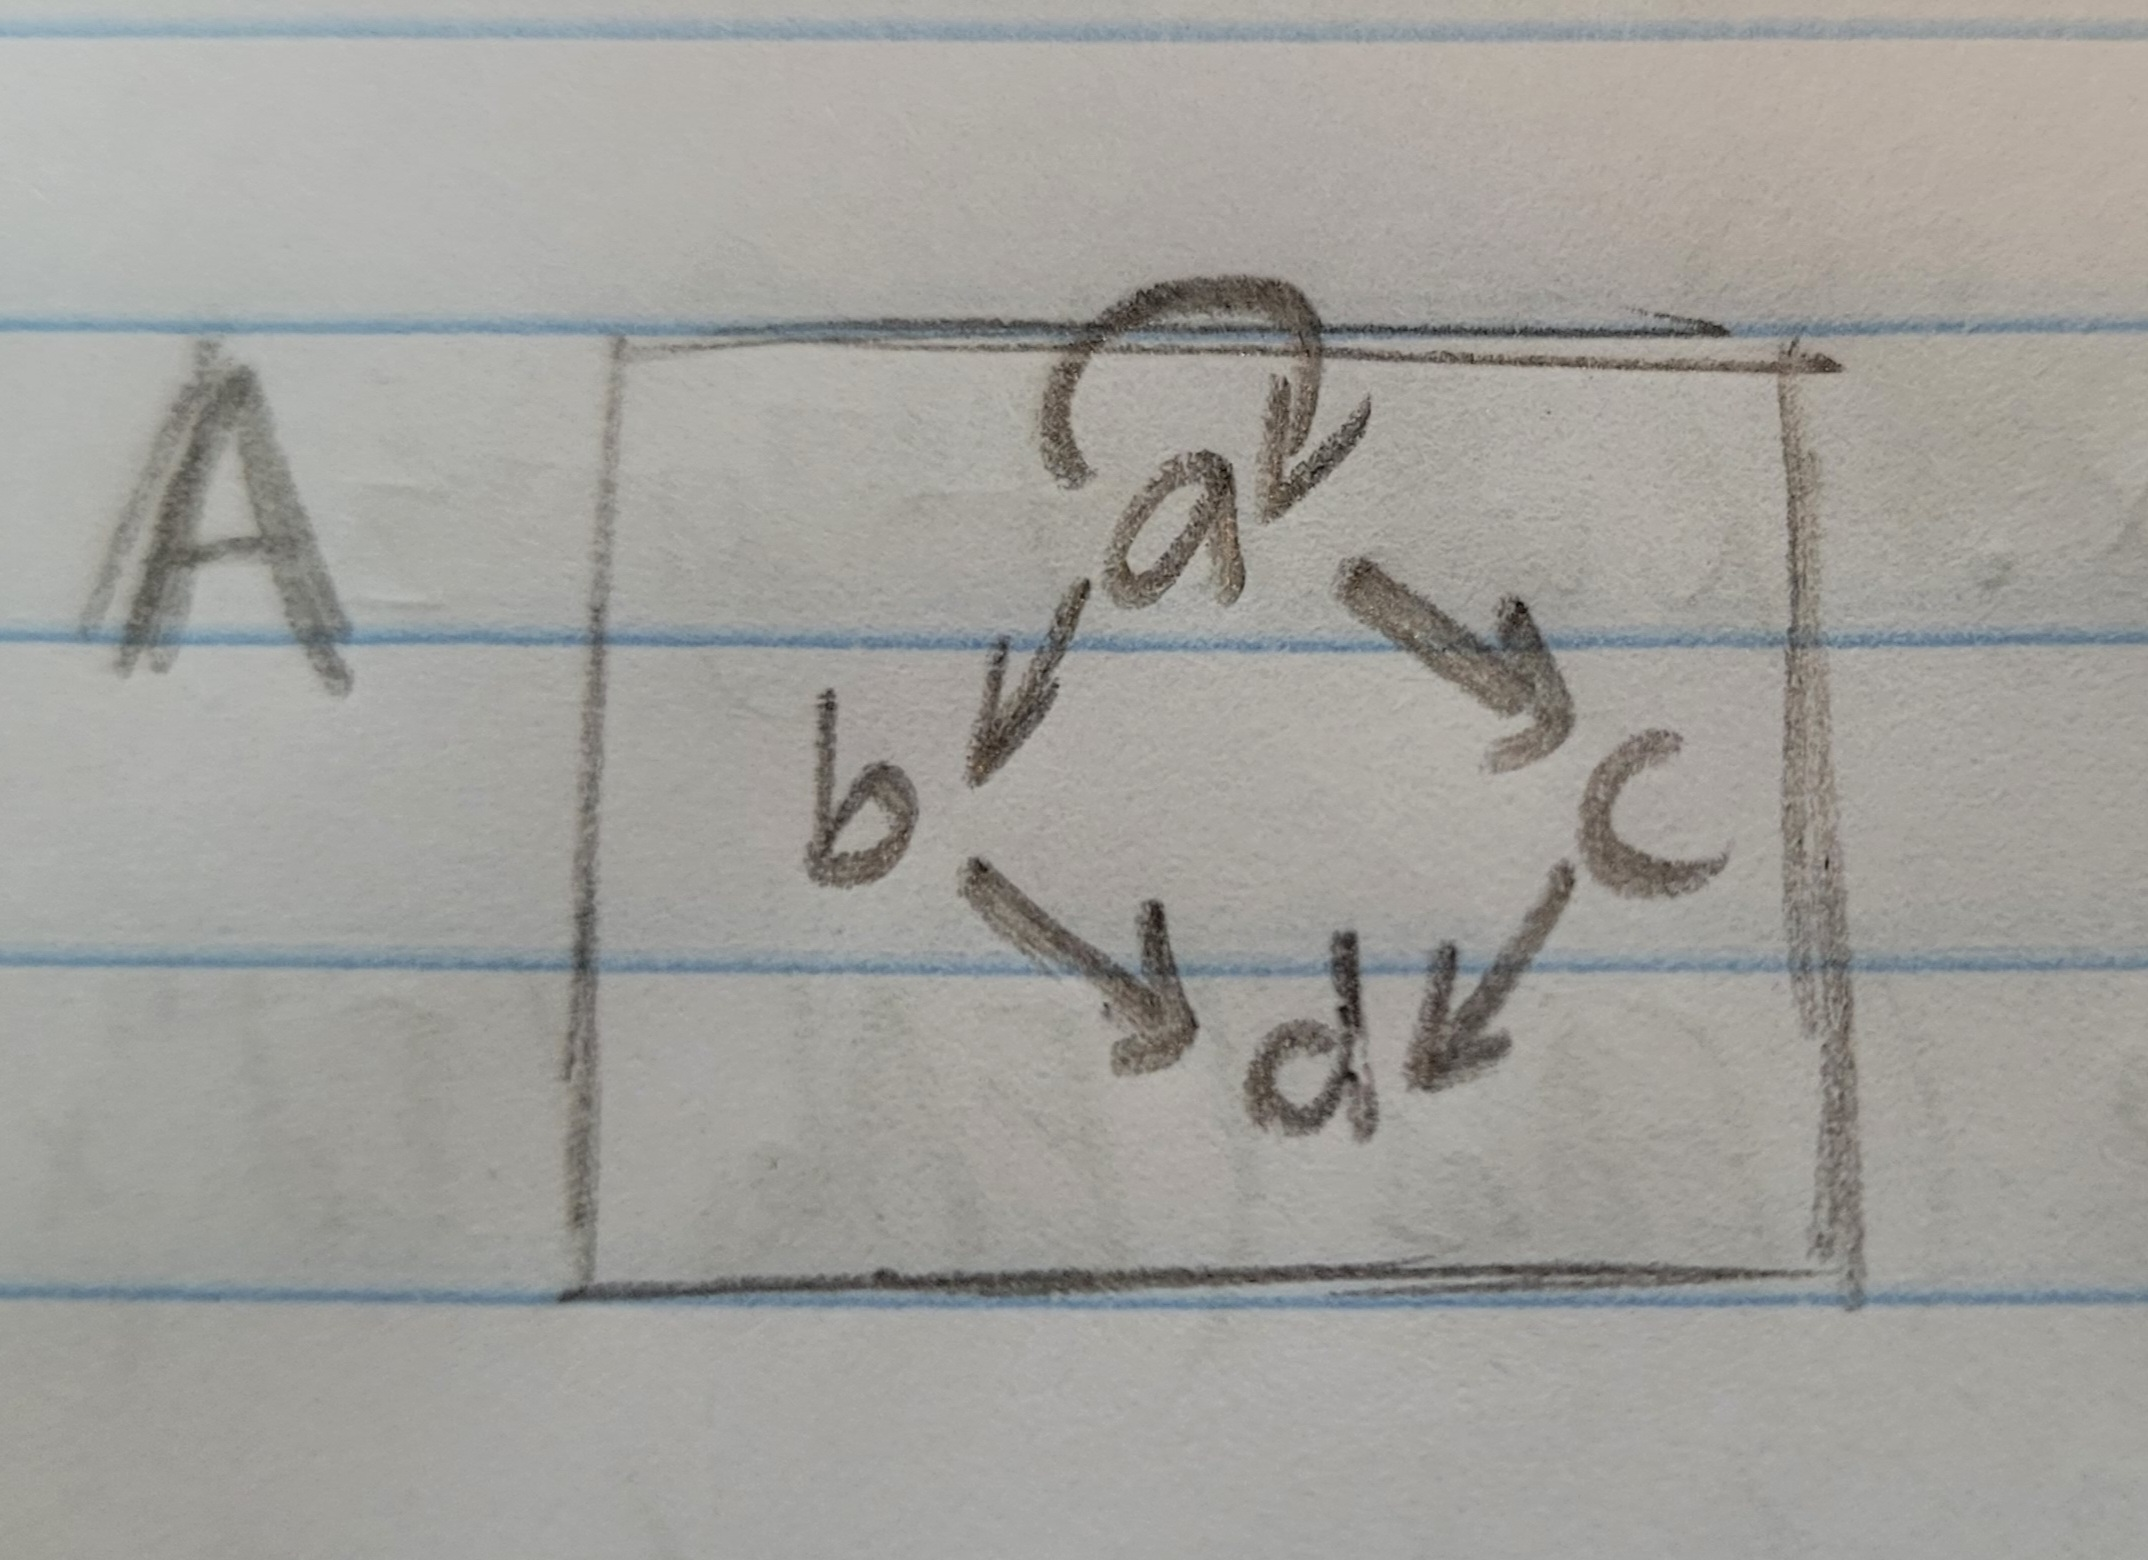
\includegraphics[width=15cm, height=8cm]{Report Images/week7_9.jpg}
\\ 4. Confluent: True, Terminating: False, Unique Normal Forms: False
\\ a points to itself, add picture later
\\ 5. Confluent: False, Terminating: True, Unique Normal Forms: True
\\ There is no example of this as in order for there to be a possibility of having an Unique Normal Form, the ARS must be at the very least Confluent, making "Confluence: False" an impossibility to have alongside "Unique Normal Form: False."
\\ 6. Confluent: False, Terminating: True, Unique Normal Forms: False
\\ 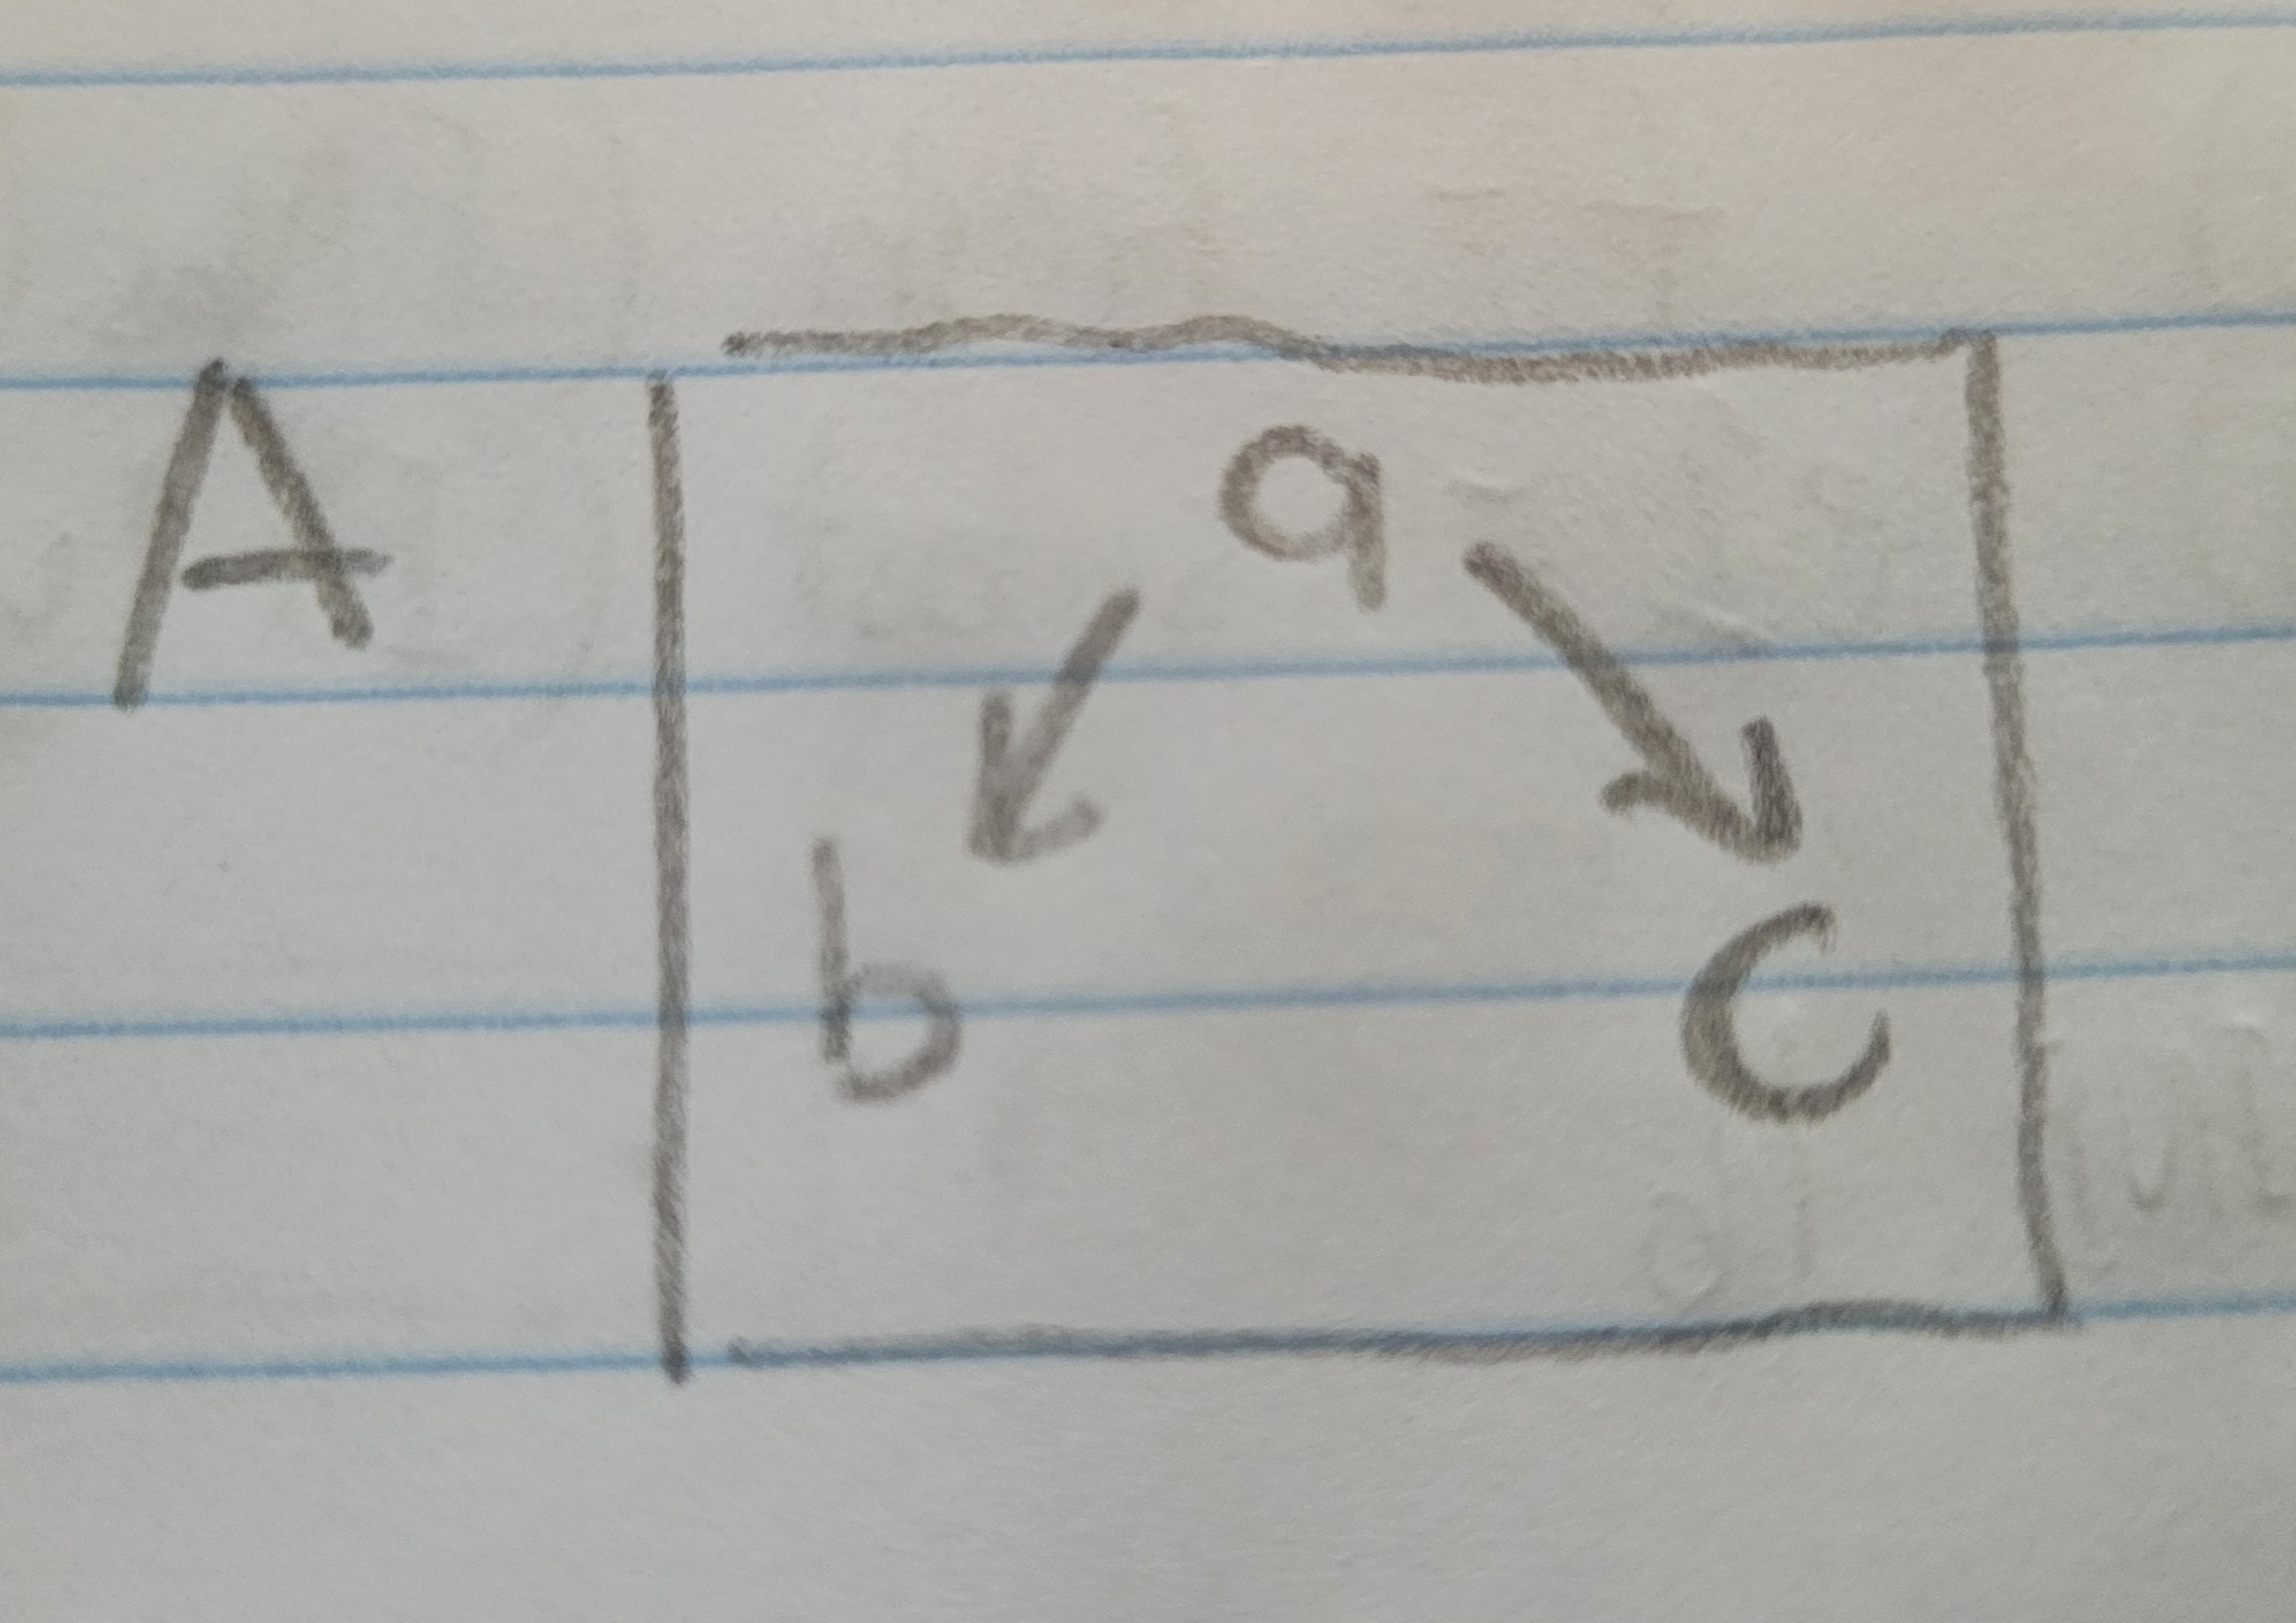
\includegraphics[width=15cm, height=8cm]{Report Images/week7_11.jpg}
\\ 7. Confluent: False, Terminating: False, Unique Normal Forms: True
\\ There is no example of this as in order for an ARS to have a Unique Normal Form, at its base, the ARS must be at least Confluent, making "Confluence: False" an impossibility to have alongside "Unique Normal Form: True."
\\ 8. Confluent: False, Terminating: False, Unique Normal Forms: False
\\ 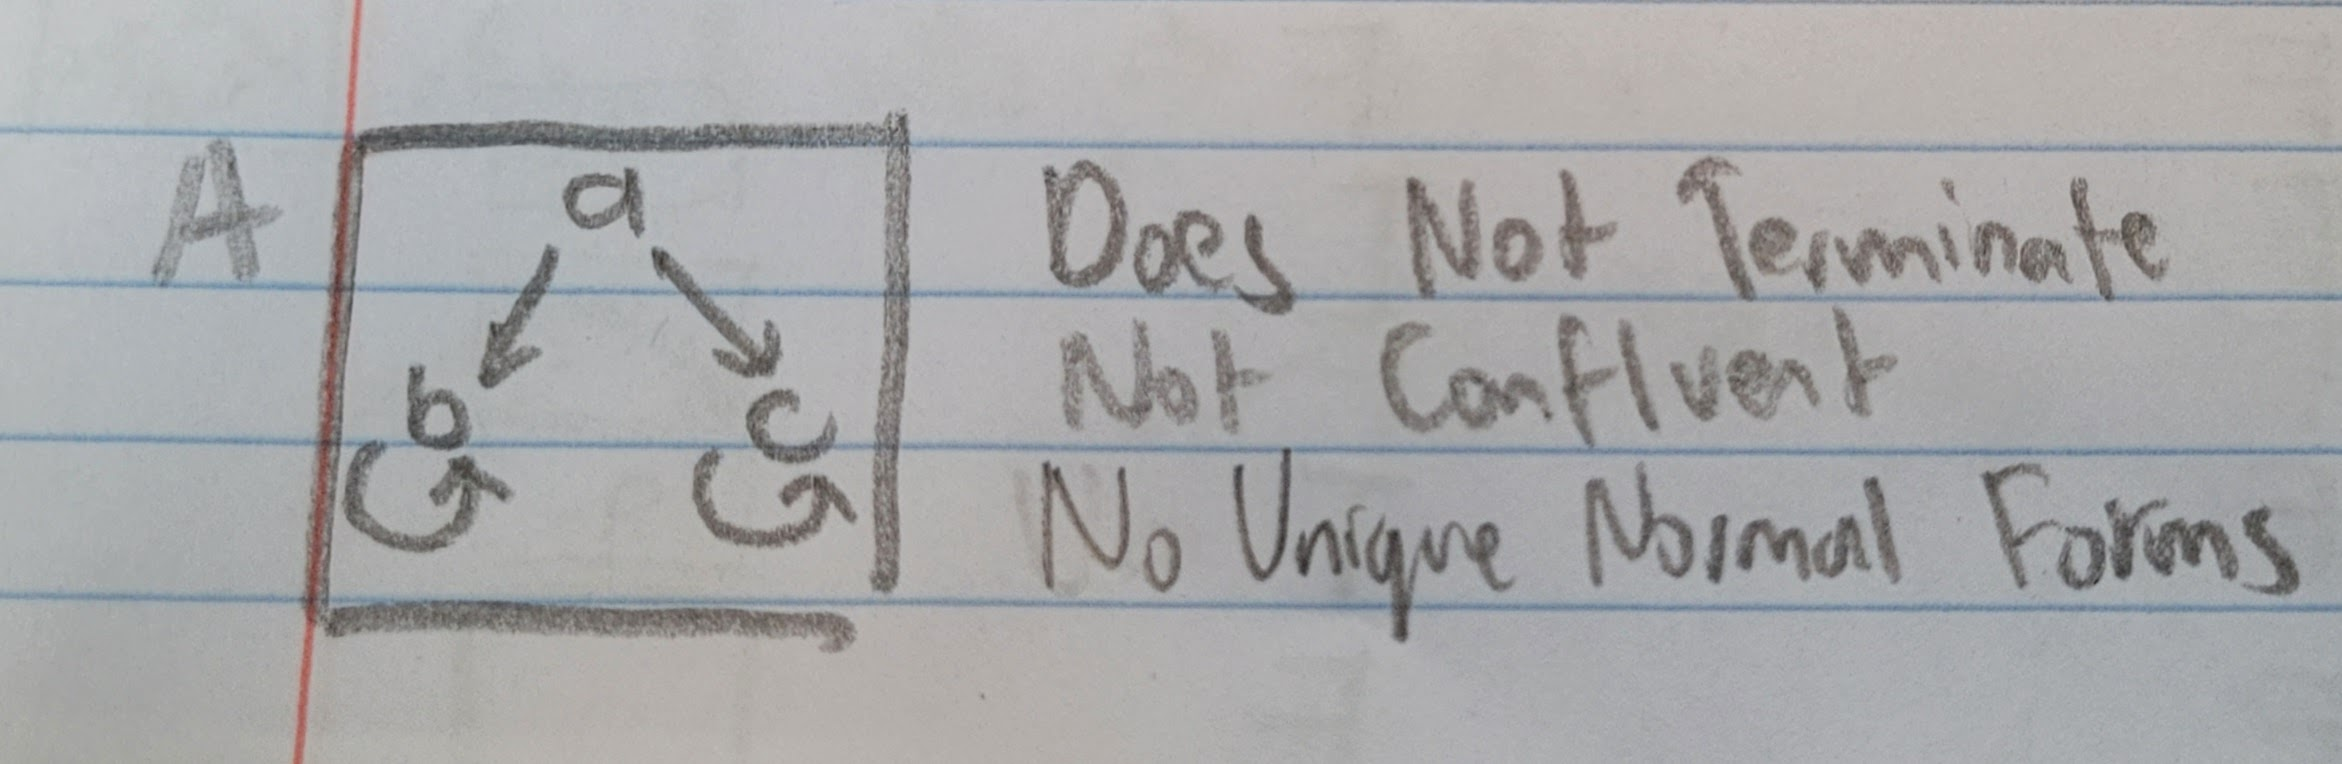
\includegraphics[width=15cm, height=8cm]{Report Images/week7_7.jpg}
\subsection{Week 8}
For the rewrite rules:
\begin{lstlisting}
  aa -> a
  bb -> b
  ba -> ab
  ab -> ba
\end{lstlisting}
\begin{enumerate}
    \item The ARS does not terminate because the output of the last rewrite rule is the input of the third rewrite rule, and the output of the third rule is the input of the last rule. This results in the potential for an infinitely rewriting function, and thus the ARS does not terminate.
    \item The normal forms of this ARS are \textit{a} and \textit{b}.
    \item The main change that would be made to the function would be to eliminate the fourth rule. Thus the ARS would have 3 normal forms: \textit{a}, \textit{b}, and \textit{ab}.
    \item The normal forms within the context of the ARS are a single form of a duplicate term. Because of this, it can be said that the primary function of the ARS is to reduce any duplicate terms until there are no longer any duplicates.
\end{enumerate}
\subsection{Week 9}
\textbf{Project Milestones}
\begin{enumerate}
    \item By \textbf{November 5, 2022}, email Dr. Kurtz the questions regarding the Programming Languages GitHub Data for the report, as well as the Excel sheet based on the data found from Githut.info.
    \begin{itemize}
        \item There should at least be \textbf{three} data analysis-related questions.
        \item The questions should relate to different types of statistical models, or involve the modification of a previously used statistical model using another data analysis technique.
        \item The questions should have some relation to the nature or ask for some conclusion about Programming Languages based on the resulting statistical model.
        \item This can alternatively be found uploaded to the \textit{Programming Languages Project Documents} folder on GitHub.
    \end{itemize}
    \item By \textbf{November 19, 2022}, create the statistical models associated for each of the questions.
    \begin{itemize}
        \item This will be accomplished via Google Colab
        \item The code and associated models for each of the statistical models should be included within the \textbf{Prototype} subsection of this report.
        \item Justifications for certain choices when generating the models (i.e. selecting a specific clustering methods or selecting which variables should be excluded from a revised model) should be also included alongside the code for the statistical models as comments.
        \item The Colab Notebook and a PDF of the compiled Notebook containing the statistical models should be uploaded to the \textit{Programming Languages Project Documents} folder on GitHub.
    \end{itemize}
    \item By \textbf{December 3, 2022}, have a rough draft of the responses to each of the questions for this report.
    \begin{itemize}
        \item This can be either written in a Word Document uploaded to the \textit{Programming Languages Project Documents} folder on GitHub or written directly to the \textbf{Documentation} section of this report.
        \item The responses to each of the questions, while still answering the questions, should contain a clear connection and come to a conclusion about trends and observations that can be made regarding the Programming Languages data.
        \item Justifications for decisions made regarding why certain modelling techniques or variables get excluded should also be reiterated within the report.
    \end{itemize}
\end{enumerate}
For the ARS (A, $\xrightarrow{}$) where A is the set of words over the alphabet ${a, b, c}$ and defined by the rules:
\begin{lstlisting}
ba -> ab
ab -> ba
ac -> ca
ca -> ac
bc -> cb
cb -> bc

aa -> b
ab -> c
ac ->
bb ->
cb -> a
cc -> b
\end{lstlisting}
The first six rules of the ARS indicate that the order of each member of the alphabet within a word does not matter, as each word can be rewritten into any other word containing the same letters. Consequently, the first six rules also show that the ARS does not necessarily terminate, due to being able to a potential to be rearranged infinitely. The last six rules of the ARS on the other hand, show that the ARS does actually have normal forms, which happen to be \textit{a}, \textit{b}, \textit{c}, and \textit{blank}. While the seventh, eighth, eleventh, and twelfth rules of the ARS indicate that if there are an even number of members within the starting word, that the ARS will result in a single member being the normal form of the ARS, the ninth and tenth rules of the ARS imply that in the event that the starting word has an odd number of members, that the resulting normal form of the ARS would be blank. Because of this, while the ARS may have normal forms, none of them are unique to the ARS. Because this ARS has multiple normal forms, it is not necessarily confluent either as the only case that it would be confluent is where the initial word has an odd number of members.
\subsection{Week 10}
Given \textit{F} as:
\begin{lstlisting}
\f. \n. if n == 0 then 1 else f(n-1)*n
\end{lstlisting}
Reduction of $fix\textsubscript{F}2$, which is equivalent to $Ff\textsubscript{fix}2$:
\begin{lstlisting}
f2 =
    fixF 2 =
    F fixF 2 =
    -- Haskell is lazy and evaluates F first
    (\f. \n. if n == 0 then 1 else f(n-1) * n) FixF 2 =
    if 2 == 0 then 1 else fixF (2-1) * 2 =
    -- else case
    (fixF 1) * 2 =
    -- 2 can be moved to the left-hand side, while fixF 1 becomes F fixF 1, and Haskell evaluates F first
    2 * (\f. \n. if n == 0 then 1 else f(n-1) * n) FixF 1 =
    2 * (if 1 == 0 then 1 else fixF (1-1) * 1) =
    -- else case
    2 * ((fixF 0) * 1) =
    -- 1 can be moved to the left-hand side, while fixF 0 becomes F fixF1, and Haskell evaluates F first
    2 * 1 * (\f. \n. if n == 0 then 1 else f(n-1) * n) FixF 0 =
    2 * 1 * (if 0 == 0 then 1 else fixF(0) * 0) FixF -1 =
    -- then case
    2 * 1 * 1 =
    2
\end{lstlisting}

\section{Project}\label{Project}
\subsection{Specification}
For my project in Programming Languages (Fall 2022), I intend on performing data analysis on a data set that is publicly available from GitHub. To accomplish this, the following would have to occur (in order):
\begin{enumerate}
    \item Receive approval from Dr. Kurtz for this specific project idea
    \item Come up with specific questions to answer about the Programming Languages data set, the responses to which can be modeled through various statistical models such as Linear/Logistic Regression Graphs, Data Cluster Graphs, Feature Reduction, LASSO Graphs, and/or Principle Component Analysis (PCA)
    \item Receive approval from Dr. Kurtz about the questions and the overall documentation of the data analysis report
    \item Download or import the data set from GitHub into Google Colab, this can be accomplished by replicating a specific iteration of the GitHub Programming Languages data set in an Excel sheet
    \item Using the Pandas package for Python, create statistical models to respond to each of the questions created for the report
    \item By the last day of October, provide a PDF of the Google Colab Notebook containing the compiled statistical models as a proof of implementation for this project. This can also be accomplished by embedding the Python code into the "Prototype" subsection of \textit{report.tex}, with each code block being above the respective model that it generated when compiled
    \item Write report for the analysis of the data set itself, explaining the process of selecting which model(s) to accept, reject, or if any model provided any surprising results about the data set in addition to providing a response to each of the questions created from \textbf{step 4}. A rough draft of this report should be submitted and present within the "Documentation" subsection of \textit{report.tex}
\end{enumerate}
\subsection{Prototype}
\subsection{Documentation}
\subsection{Critical Appraisal}

\section{Conclusions}\label{Conclusions}
\dots
\end{document}
